% Options for packages loaded elsewhere
\PassOptionsToPackage{unicode}{hyperref}
\PassOptionsToPackage{hyphens}{url}
\PassOptionsToPackage{dvipsnames,svgnames,x11names}{xcolor}
%
\documentclass[
  letterpaper,
  DIV=11,
  numbers=noendperiod]{scrreprt}

\usepackage{amsmath,amssymb}
\usepackage{iftex}
\ifPDFTeX
  \usepackage[T1]{fontenc}
  \usepackage[utf8]{inputenc}
  \usepackage{textcomp} % provide euro and other symbols
\else % if luatex or xetex
  \usepackage{unicode-math}
  \defaultfontfeatures{Scale=MatchLowercase}
  \defaultfontfeatures[\rmfamily]{Ligatures=TeX,Scale=1}
\fi
\usepackage[]{cochineal}
\ifPDFTeX\else  
    % xetex/luatex font selection
\fi
% Use upquote if available, for straight quotes in verbatim environments
\IfFileExists{upquote.sty}{\usepackage{upquote}}{}
\IfFileExists{microtype.sty}{% use microtype if available
  \usepackage[]{microtype}
  \UseMicrotypeSet[protrusion]{basicmath} % disable protrusion for tt fonts
}{}
\makeatletter
\@ifundefined{KOMAClassName}{% if non-KOMA class
  \IfFileExists{parskip.sty}{%
    \usepackage{parskip}
  }{% else
    \setlength{\parindent}{0pt}
    \setlength{\parskip}{6pt plus 2pt minus 1pt}}
}{% if KOMA class
  \KOMAoptions{parskip=half}}
\makeatother
\usepackage{xcolor}
\setlength{\emergencystretch}{3em} % prevent overfull lines
\setcounter{secnumdepth}{5}
% Make \paragraph and \subparagraph free-standing
\ifx\paragraph\undefined\else
  \let\oldparagraph\paragraph
  \renewcommand{\paragraph}[1]{\oldparagraph{#1}\mbox{}}
\fi
\ifx\subparagraph\undefined\else
  \let\oldsubparagraph\subparagraph
  \renewcommand{\subparagraph}[1]{\oldsubparagraph{#1}\mbox{}}
\fi

\usepackage{color}
\usepackage{fancyvrb}
\newcommand{\VerbBar}{|}
\newcommand{\VERB}{\Verb[commandchars=\\\{\}]}
\DefineVerbatimEnvironment{Highlighting}{Verbatim}{commandchars=\\\{\}}
% Add ',fontsize=\small' for more characters per line
\usepackage{framed}
\definecolor{shadecolor}{RGB}{241,243,245}
\newenvironment{Shaded}{\begin{snugshade}}{\end{snugshade}}
\newcommand{\AlertTok}[1]{\textcolor[rgb]{0.68,0.00,0.00}{#1}}
\newcommand{\AnnotationTok}[1]{\textcolor[rgb]{0.37,0.37,0.37}{#1}}
\newcommand{\AttributeTok}[1]{\textcolor[rgb]{0.40,0.45,0.13}{#1}}
\newcommand{\BaseNTok}[1]{\textcolor[rgb]{0.68,0.00,0.00}{#1}}
\newcommand{\BuiltInTok}[1]{\textcolor[rgb]{0.00,0.23,0.31}{#1}}
\newcommand{\CharTok}[1]{\textcolor[rgb]{0.13,0.47,0.30}{#1}}
\newcommand{\CommentTok}[1]{\textcolor[rgb]{0.37,0.37,0.37}{#1}}
\newcommand{\CommentVarTok}[1]{\textcolor[rgb]{0.37,0.37,0.37}{\textit{#1}}}
\newcommand{\ConstantTok}[1]{\textcolor[rgb]{0.56,0.35,0.01}{#1}}
\newcommand{\ControlFlowTok}[1]{\textcolor[rgb]{0.00,0.23,0.31}{#1}}
\newcommand{\DataTypeTok}[1]{\textcolor[rgb]{0.68,0.00,0.00}{#1}}
\newcommand{\DecValTok}[1]{\textcolor[rgb]{0.68,0.00,0.00}{#1}}
\newcommand{\DocumentationTok}[1]{\textcolor[rgb]{0.37,0.37,0.37}{\textit{#1}}}
\newcommand{\ErrorTok}[1]{\textcolor[rgb]{0.68,0.00,0.00}{#1}}
\newcommand{\ExtensionTok}[1]{\textcolor[rgb]{0.00,0.23,0.31}{#1}}
\newcommand{\FloatTok}[1]{\textcolor[rgb]{0.68,0.00,0.00}{#1}}
\newcommand{\FunctionTok}[1]{\textcolor[rgb]{0.28,0.35,0.67}{#1}}
\newcommand{\ImportTok}[1]{\textcolor[rgb]{0.00,0.46,0.62}{#1}}
\newcommand{\InformationTok}[1]{\textcolor[rgb]{0.37,0.37,0.37}{#1}}
\newcommand{\KeywordTok}[1]{\textcolor[rgb]{0.00,0.23,0.31}{#1}}
\newcommand{\NormalTok}[1]{\textcolor[rgb]{0.00,0.23,0.31}{#1}}
\newcommand{\OperatorTok}[1]{\textcolor[rgb]{0.37,0.37,0.37}{#1}}
\newcommand{\OtherTok}[1]{\textcolor[rgb]{0.00,0.23,0.31}{#1}}
\newcommand{\PreprocessorTok}[1]{\textcolor[rgb]{0.68,0.00,0.00}{#1}}
\newcommand{\RegionMarkerTok}[1]{\textcolor[rgb]{0.00,0.23,0.31}{#1}}
\newcommand{\SpecialCharTok}[1]{\textcolor[rgb]{0.37,0.37,0.37}{#1}}
\newcommand{\SpecialStringTok}[1]{\textcolor[rgb]{0.13,0.47,0.30}{#1}}
\newcommand{\StringTok}[1]{\textcolor[rgb]{0.13,0.47,0.30}{#1}}
\newcommand{\VariableTok}[1]{\textcolor[rgb]{0.07,0.07,0.07}{#1}}
\newcommand{\VerbatimStringTok}[1]{\textcolor[rgb]{0.13,0.47,0.30}{#1}}
\newcommand{\WarningTok}[1]{\textcolor[rgb]{0.37,0.37,0.37}{\textit{#1}}}

\providecommand{\tightlist}{%
  \setlength{\itemsep}{0pt}\setlength{\parskip}{0pt}}\usepackage{longtable,booktabs,array}
\usepackage{calc} % for calculating minipage widths
% Correct order of tables after \paragraph or \subparagraph
\usepackage{etoolbox}
\makeatletter
\patchcmd\longtable{\par}{\if@noskipsec\mbox{}\fi\par}{}{}
\makeatother
% Allow footnotes in longtable head/foot
\IfFileExists{footnotehyper.sty}{\usepackage{footnotehyper}}{\usepackage{footnote}}
\makesavenoteenv{longtable}
\usepackage{graphicx}
\makeatletter
\def\maxwidth{\ifdim\Gin@nat@width>\linewidth\linewidth\else\Gin@nat@width\fi}
\def\maxheight{\ifdim\Gin@nat@height>\textheight\textheight\else\Gin@nat@height\fi}
\makeatother
% Scale images if necessary, so that they will not overflow the page
% margins by default, and it is still possible to overwrite the defaults
% using explicit options in \includegraphics[width, height, ...]{}
\setkeys{Gin}{width=\maxwidth,height=\maxheight,keepaspectratio}
% Set default figure placement to htbp
\makeatletter
\def\fps@figure{htbp}
\makeatother
\newlength{\cslhangindent}
\setlength{\cslhangindent}{1.5em}
\newlength{\csllabelwidth}
\setlength{\csllabelwidth}{3em}
\newlength{\cslentryspacingunit} % times entry-spacing
\setlength{\cslentryspacingunit}{\parskip}
\newenvironment{CSLReferences}[2] % #1 hanging-ident, #2 entry spacing
 {% don't indent paragraphs
  \setlength{\parindent}{0pt}
  % turn on hanging indent if param 1 is 1
  \ifodd #1
  \let\oldpar\par
  \def\par{\hangindent=\cslhangindent\oldpar}
  \fi
  % set entry spacing
  \setlength{\parskip}{#2\cslentryspacingunit}
 }%
 {}
\usepackage{calc}
\newcommand{\CSLBlock}[1]{#1\hfill\break}
\newcommand{\CSLLeftMargin}[1]{\parbox[t]{\csllabelwidth}{#1}}
\newcommand{\CSLRightInline}[1]{\parbox[t]{\linewidth - \csllabelwidth}{#1}\break}
\newcommand{\CSLIndent}[1]{\hspace{\cslhangindent}#1}

\newcommand{\bs}{\symbf}
\newcommand{\mb}{\symbf}
\newcommand{\E}{\mathbb{E}}
\newcommand{\V}{\mathbb{V}}
\newcommand{\var}{\text{var}}
\newcommand{\cov}{\text{cov}}
\newcommand{\N}{\mathcal{N}}
\newcommand{\Bern}{\text{Bern}}
\newcommand{\Bin}{\text{Bin}}
\newcommand{\Pois}{\text{Pois}}
\newcommand{\Unif}{\text{Unif}}
\newcommand{\se}{\textsf{se}}
\newcommand{\au}{\underline{a}}
\newcommand{\du}{\underline{d}}
\newcommand{\Au}{\underline{A}}
\newcommand{\Du}{\underline{D}}
\newcommand{\xu}{\underline{x}}
\newcommand{\Xu}{\underline{X}}
\newcommand{\Yu}{\underline{Y}}
\renewcommand{\P}{\mathbb{P}}
\newcommand{\U}{\mb{U}}
\newcommand{\Xbar}{\overline{X}}
\newcommand{\Ybar}{\overline{Y}}
\newcommand{\real}{\mathbb{R}}
\newcommand{\bbL}{\mathbb{L}}
\renewcommand{\u}{\mb{u}}
\renewcommand{\v}{\mb{v}}
\newcommand{\M}{\mb{M}}
\newcommand{\X}{\mb{X}}
\newcommand{\Xmat}{\mathbb{X}}
\newcommand{\bfx}{\mb{x}}
\newcommand{\y}{\mb{y}}
\newcommand{\bfbeta}{\mb{\beta}}
\renewcommand{\b}{\symbf{\beta}}
\newcommand{\e}{\bs{\epsilon}}
\newcommand{\bhat}{\widehat{\mb{\beta}}}
\newcommand{\XX}{\Xmat'\Xmat}
\newcommand{\XXinv}{\left(\XX\right)^{-1}}
\newcommand{\hatsig}{\hat{\sigma}^2}
\newcommand{\red}[1]{\textcolor{red!60}{#1}}
\newcommand{\indianred}[1]{\textcolor{indianred}{#1}}
\newcommand{\blue}[1]{\textcolor{blue!60}{#1}}
\newcommand{\dblue}[1]{\textcolor{dodgerblue}{#1}}
\newcommand{\indep}{\perp\!\!\!\perp}
\newcommand{\inprob}{\overset{p}{\to}}
\newcommand{\indist}{\overset{d}{\to}}
\newcommand{\eframe}{\end{frame}}
\newcommand{\bframe}{\begin{frame}}
\newcommand{\R}{\textsf{\textbf{R}}}
\newcommand{\Rst}{\textsf{\textbf{RStudio}}}
\newcommand{\rfun}[1]{\texttt{\color{magenta}{#1}}}
\newcommand{\rpack}[1]{\textbf{#1}}
\newcommand{\rexpr}[1]{\texttt{\color{magenta}{#1}}}
\newcommand{\filename}[1]{\texttt{\color{blue}{#1}}}
\DeclareMathOperator*{\argmax}{arg\,max}
\DeclareMathOperator*{\argmin}{arg\,min}
\KOMAoption{captions}{tableheading}
\makeatletter
\@ifpackageloaded{tcolorbox}{}{\usepackage[skins,breakable]{tcolorbox}}
\@ifpackageloaded{fontawesome5}{}{\usepackage{fontawesome5}}
\definecolor{quarto-callout-color}{HTML}{909090}
\definecolor{quarto-callout-note-color}{HTML}{0758E5}
\definecolor{quarto-callout-important-color}{HTML}{CC1914}
\definecolor{quarto-callout-warning-color}{HTML}{EB9113}
\definecolor{quarto-callout-tip-color}{HTML}{00A047}
\definecolor{quarto-callout-caution-color}{HTML}{FC5300}
\definecolor{quarto-callout-color-frame}{HTML}{acacac}
\definecolor{quarto-callout-note-color-frame}{HTML}{4582ec}
\definecolor{quarto-callout-important-color-frame}{HTML}{d9534f}
\definecolor{quarto-callout-warning-color-frame}{HTML}{f0ad4e}
\definecolor{quarto-callout-tip-color-frame}{HTML}{02b875}
\definecolor{quarto-callout-caution-color-frame}{HTML}{fd7e14}
\makeatother
\makeatletter
\makeatother
\makeatletter
\@ifpackageloaded{bookmark}{}{\usepackage{bookmark}}
\makeatother
\makeatletter
\@ifpackageloaded{caption}{}{\usepackage{caption}}
\AtBeginDocument{%
\ifdefined\contentsname
  \renewcommand*\contentsname{Table of contents}
\else
  \newcommand\contentsname{Table of contents}
\fi
\ifdefined\listfigurename
  \renewcommand*\listfigurename{List of Figures}
\else
  \newcommand\listfigurename{List of Figures}
\fi
\ifdefined\listtablename
  \renewcommand*\listtablename{List of Tables}
\else
  \newcommand\listtablename{List of Tables}
\fi
\ifdefined\figurename
  \renewcommand*\figurename{Figure}
\else
  \newcommand\figurename{Figure}
\fi
\ifdefined\tablename
  \renewcommand*\tablename{Table}
\else
  \newcommand\tablename{Table}
\fi
}
\@ifpackageloaded{float}{}{\usepackage{float}}
\floatstyle{ruled}
\@ifundefined{c@chapter}{\newfloat{codelisting}{h}{lop}}{\newfloat{codelisting}{h}{lop}[chapter]}
\floatname{codelisting}{Listing}
\newcommand*\listoflistings{\listof{codelisting}{List of Listings}}
\usepackage{amsthm}
\theoremstyle{definition}
\newtheorem{definition}{Definition}[chapter]
\theoremstyle{definition}
\newtheorem{example}{Example}[chapter]
\theoremstyle{plain}
\newtheorem{theorem}{Theorem}[chapter]
\theoremstyle{remark}
\AtBeginDocument{\renewcommand*{\proofname}{Proof}}
\newtheorem*{remark}{Remark}
\newtheorem*{solution}{Solution}
\makeatother
\makeatletter
\@ifpackageloaded{caption}{}{\usepackage{caption}}
\@ifpackageloaded{subcaption}{}{\usepackage{subcaption}}
\makeatother
\makeatletter
\@ifpackageloaded{tcolorbox}{}{\usepackage[skins,breakable]{tcolorbox}}
\makeatother
\makeatletter
\@ifundefined{shadecolor}{\definecolor{shadecolor}{rgb}{.97, .97, .97}}
\makeatother
\makeatletter
\makeatother
\makeatletter
\makeatother
\ifLuaTeX
  \usepackage{selnolig}  % disable illegal ligatures
\fi
\IfFileExists{bookmark.sty}{\usepackage{bookmark}}{\usepackage{hyperref}}
\IfFileExists{xurl.sty}{\usepackage{xurl}}{} % add URL line breaks if available
\urlstyle{same} % disable monospaced font for URLs
\hypersetup{
  pdftitle={A User's Guide to Statistical Inference and Regression},
  pdfauthor={Matthew Blackwell},
  colorlinks=true,
  linkcolor={blue},
  filecolor={Maroon},
  citecolor={Blue},
  urlcolor={Blue},
  pdfcreator={LaTeX via pandoc}}

\title{A User's Guide to Statistical Inference and Regression}
\author{Matthew Blackwell}
\date{}

\begin{document}
\maketitle
\ifdefined\Shaded\renewenvironment{Shaded}{\begin{tcolorbox}[sharp corners, breakable, enhanced, boxrule=0pt, borderline west={3pt}{0pt}{shadecolor}, frame hidden, interior hidden]}{\end{tcolorbox}}\fi

\renewcommand*\contentsname{Table of contents}
{
\hypersetup{linkcolor=}
\setcounter{tocdepth}{2}
\tableofcontents
}
\bookmarksetup{startatroot}

\hypertarget{preface}{%
\chapter*{Preface}\label{preface}}
\addcontentsline{toc}{chapter}{Preface}

\markboth{Preface}{Preface}

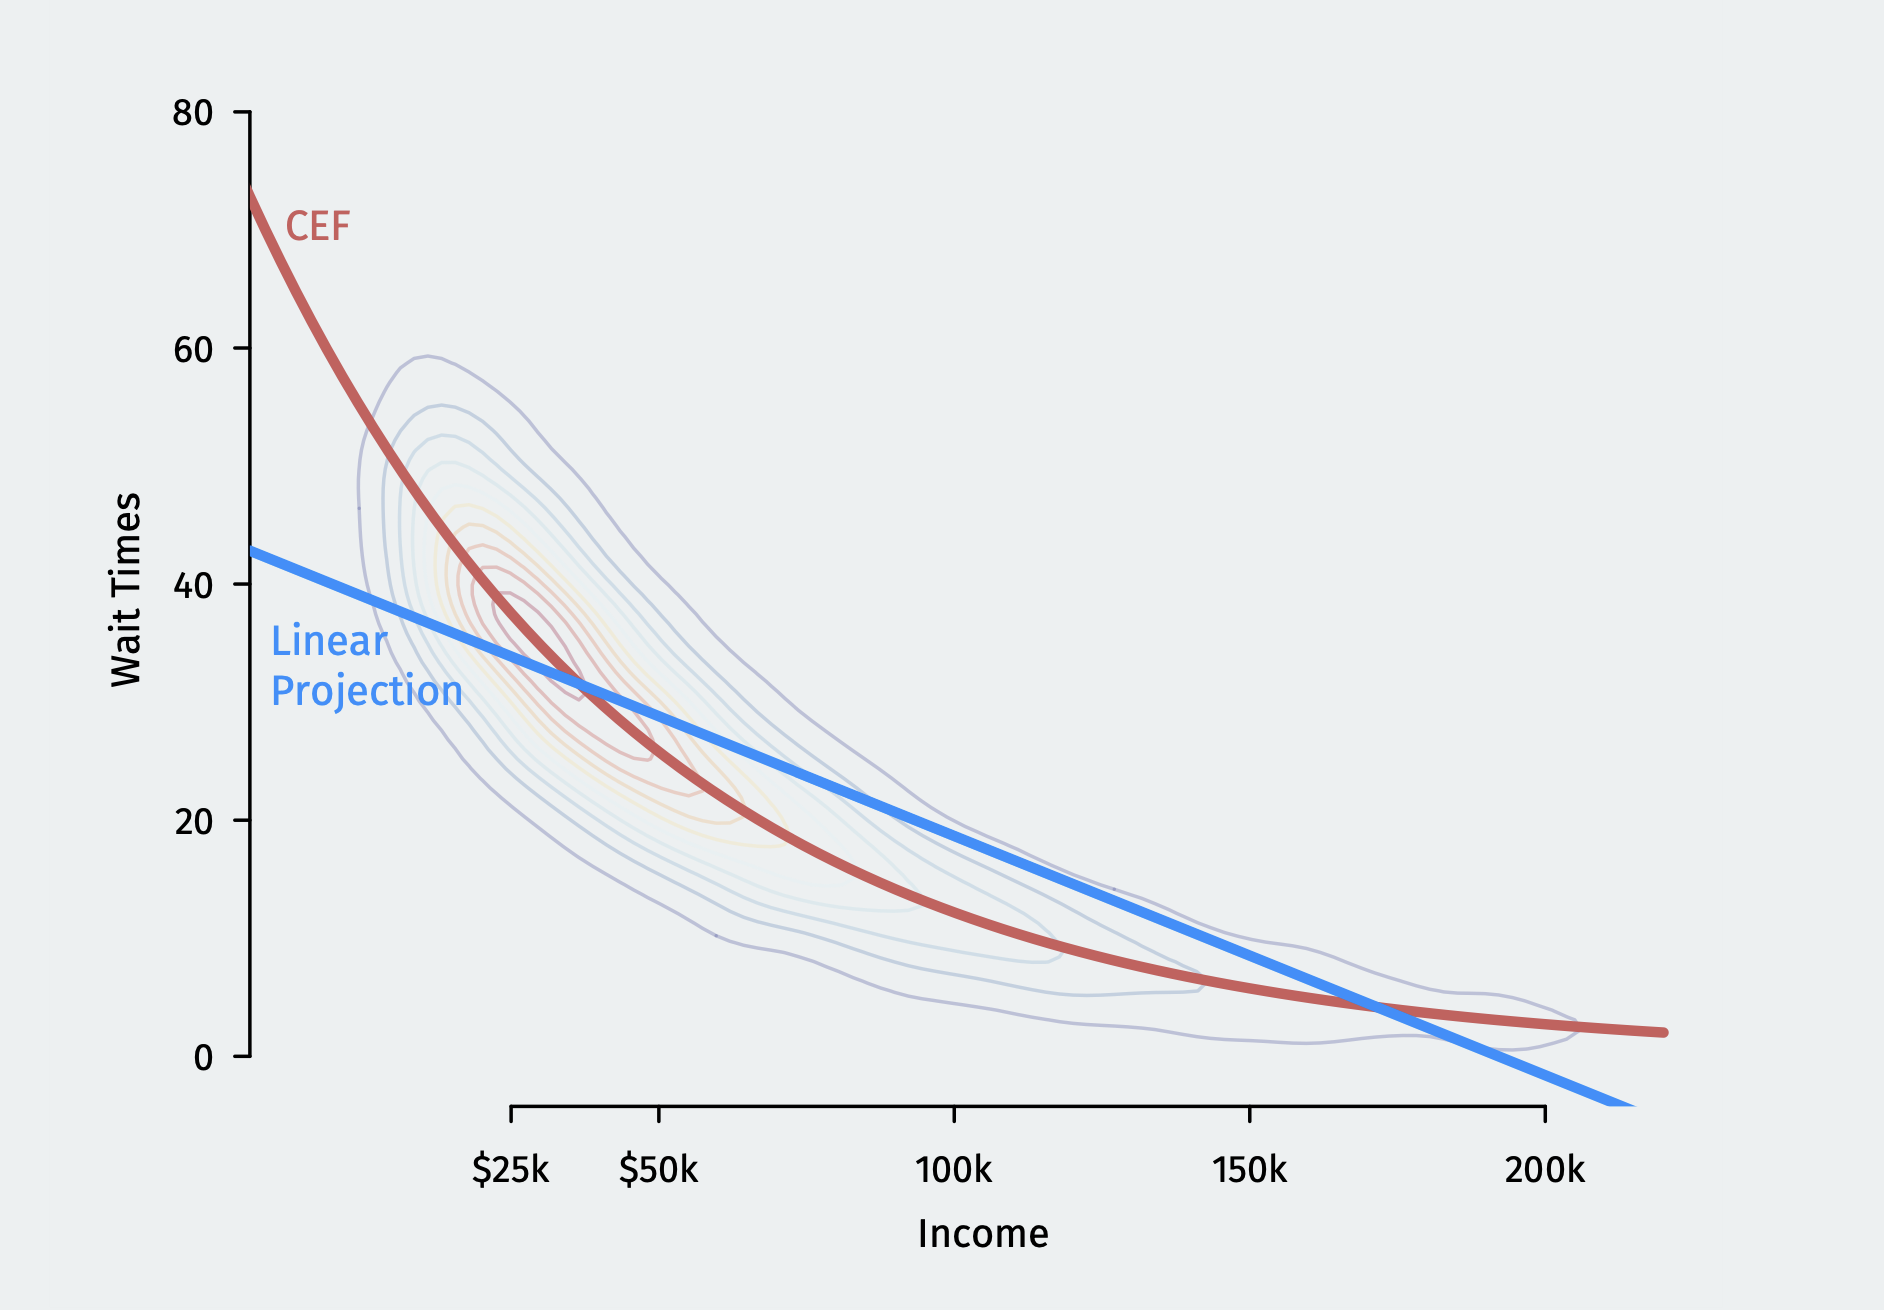
\includegraphics{assets/img/linear-approximation.png}

The goal of this text is to provide a rigorous yet accessible
introduction to the foundational topics in statistical inference with a
special application to linear regression, a workhorse tool in the social
sciences. The material is intended for first-year PhD students in
political science, but it may be of interest more broadly. Much of the
material has been adopted from various sources (far too many to recount
now), but this book is especially indebted to the following texts:

\begin{itemize}
\tightlist
\item
  Hansen, Bruce.
  \href{https://www.amazon.com/Probability-Statistics-Economists-Bruce-Hansen/dp/0691235945/}{\emph{Probability
  \& Statistics for Economists}}. Princeton University Press.
\item
  Hansen, Bruce.
  \href{https://www.amazon.com/Econometrics-Bruce-Hansen/dp/0691235899/}{\emph{Econometrics}}.
  Princeton University Press.
\item
  Wasserman, Larry.
  \href{https://link.springer.com/book/10.1007/978-0-387-21736-9}{\emph{All
  of Statistics: A Concise Course in Statistical Inference}}. Springer.
\item
  Wooldridge, Jeffrey.
  \href{https://mitpress.mit.edu/9780262232586/econometric-analysis-of-cross-section-and-panel-data/}{\emph{Econometric
  Analysis of Cross Section and Panel Data}}. The MIT Press.
\end{itemize}

You can find the source for this book at
\url{https://github.com/mattblackwell/gov2002-book}. Any typos or errors
can be reported at
\url{https://github.com/mattblackwell/gov2002-book/issues}. Thanks for
reading.

This is a Quarto book. To learn more about Quarto books visit
\url{https://quarto.org/docs/books}.

\(\,\)

\bookmarksetup{startatroot}

\hypertarget{acknowledgements}{%
\chapter*{Acknowledgements}\label{acknowledgements}}
\addcontentsline{toc}{chapter}{Acknowledgements}

\markboth{Acknowledgements}{Acknowledgements}

Much of how I approach this material comes from Adam Glynn, for whom I
was a teaching fellow during graduate school. Thanks to the students of
Gov 2000 and Gov 2002 over years for helping me refine the material in
this book. Also very special thanks to those who have provided valuable
feedback including Zeki Akyol, Noah Dasanaike, and Jarell Cheong Tze
Wen.

\bookmarksetup{startatroot}

\hypertarget{introduction}{%
\chapter{Introduction}\label{introduction}}

\(\,\)

This book, like so many books before it, will try to teach you
statistics. The field of statistics describes how we learn about the
world from quantitative data. In the social sciences, the vast majority
of empirical studies use statistical methods to provide evidence for
their arguments. While it is possible to conduct quantitative research
without understanding statistics, one must advise against it.
Quantitative research involves a host of \emph{choices} about what model
to use, what variables to include, what tuning parameters to set, what
assumptions to make, and so on. Without a deep understanding of
statistics, you will find these choices bewildering and often yield to
the default settings of your statistical software. The goal of this book
is to give you the foundation to confidently make those choices for your
specific application.

We will focus on two key goals in this book.

\begin{enumerate}
\def\labelenumi{\arabic{enumi}.}
\item
  \textbf{Understand the basic ways to assess estimators} With
  quantitative data, we often want to make statistical inferences about
  some unknown feature of the world. We use estimators (which are just
  ways of summarizing our data) to estimate these features. One major
  goal of this book is to show the basics of this task at a general
  enough level to be applicable to almost any estimator that you are
  likely to encounter in research. The ideas of bias, sampling variance,
  consistency, and asymptotic normality are common to such a large swath
  of (frequentist) inference that you get a tremendous return on your
  investment of time in these topics. Understand these core ideas and
  you will have a language to analyze any fancy new estimator that pops
  up in the next few decades.
\item
  \textbf{Apply these ideas to estimation of regressions} This book will
  apply these ideas to one particular workhorse task in the social
  sciences: estimating regression functions. So many methods either use
  regression estimators like ordinary least squares or extend it in some
  way. Understanding how these estimators work is vital for conducting
  research in the social sciences. Regression and regression estimators
  also provide an entry point for discussing parametric models
  explicitly as approximation and projections rather than as rigid
  assumptions about the truth of a given specification.
\end{enumerate}

Why write a book on statistics and regression when so many already
exist? Aside from hubris, my goal in this book is to find a level of
mathematical sophistication that will challenge and push political
scientists to develop stronger foundations in the material. While some
textbooks at this level exist in statistics and economics, they tend to
focus on applications less relevant to political science. This book
attempts to correct this.

\part{Statistical Inference}

\hypertarget{estimation}{%
\chapter{Estimation}\label{estimation}}

\hypertarget{introduction-1}{%
\section{Introduction}\label{introduction-1}}

Suppose you have been tasked with determining what fraction of a
population supports a policy of increasing legal immigration limits. You
have a sample of data on whether or not some individual respondents
support the policy. How should you use the information you know (the
data) to make a best guess about the information you don't know (the
fraction of the population)? This task is called estimation and it's the
cornerstone of most quantitative work in the social sciences.

You might think to yourself: this seems simple, just use the fraction of
the sample that supports the policy as the best guess about the fraction
of the population. And, as we'll see, under certain conditions, this
procedure is sound. The tricky part of statistics, though, is to
understand what those ``certain conditions'' are and be able to
determine if they hold in a given empirical setting. This line of
thought may lead to uncomfortable questions such as, ``where did this
sample come from?''

We begin with perhaps the simplest and most sanguine of data origin
stories: the \textbf{random sample}. The ``sample'' refers to the idea
that our data is a subset of some larger \textbf{population}. The
``random'' modifier means that the subset was chosen by an uncertain
process that did not favor one type of person versus another. Having a
random sample from a population is an example of the ``certain
conditions'' and our entry point into studying estimation in a rigorous
manner.

Why focus on random samples so much even though many data sets are at
least partially non-random or represent the entire population rather
than a subset? Consider the famous story of a drunkard's search for a
lost bill:\footnote{1924 May 24, Boston Herald, Whiting's Column:
  Tammany Has Learned That This Is No Time for Political Bosses, Quote
  Page 2, Column 1, Boston, Massachusetts. (GenealogyBank)}

\begin{quote}
``I lost a \$2 bill down on Atlantic avenue,'' said the man.

``What's that?'' asked the puzzled officer. ``You lost a \$2 bill on
Atlantic avenue? Then why are you hunting around here in Copley
square?''

``Because,'' said the man as he turned away and continued his hunt on
his hands and knees, ``the light's better up here.''
\end{quote}

Like the poor Bostonian, we focus on searching an area (random samples)
that are easier to search because there is more light or, more
accurately, easier math. Unlike this apocryphal tale, our search will
help us better understand the darkness of non-random samples, because
the core ideas and intuitions from random sampling form the basis for
the theoretical extensions into more exotic settings.

Probability is the mathematical study of uncertain events and is the
basis of the mathematical study of estimation. In probability, we assume
we know truth of the world (how many blue and red balls are in the urn)
and calculate the chances of events (getting more than give red balls
when drawing ten from the urn). Estimation works in reverse. Someone
hands you ten balls, six red and four blue, and your task is to guess
the contents of the urn from which they came. We have to use our
observed data to make an \textbf{inference} about the data-generating
process.

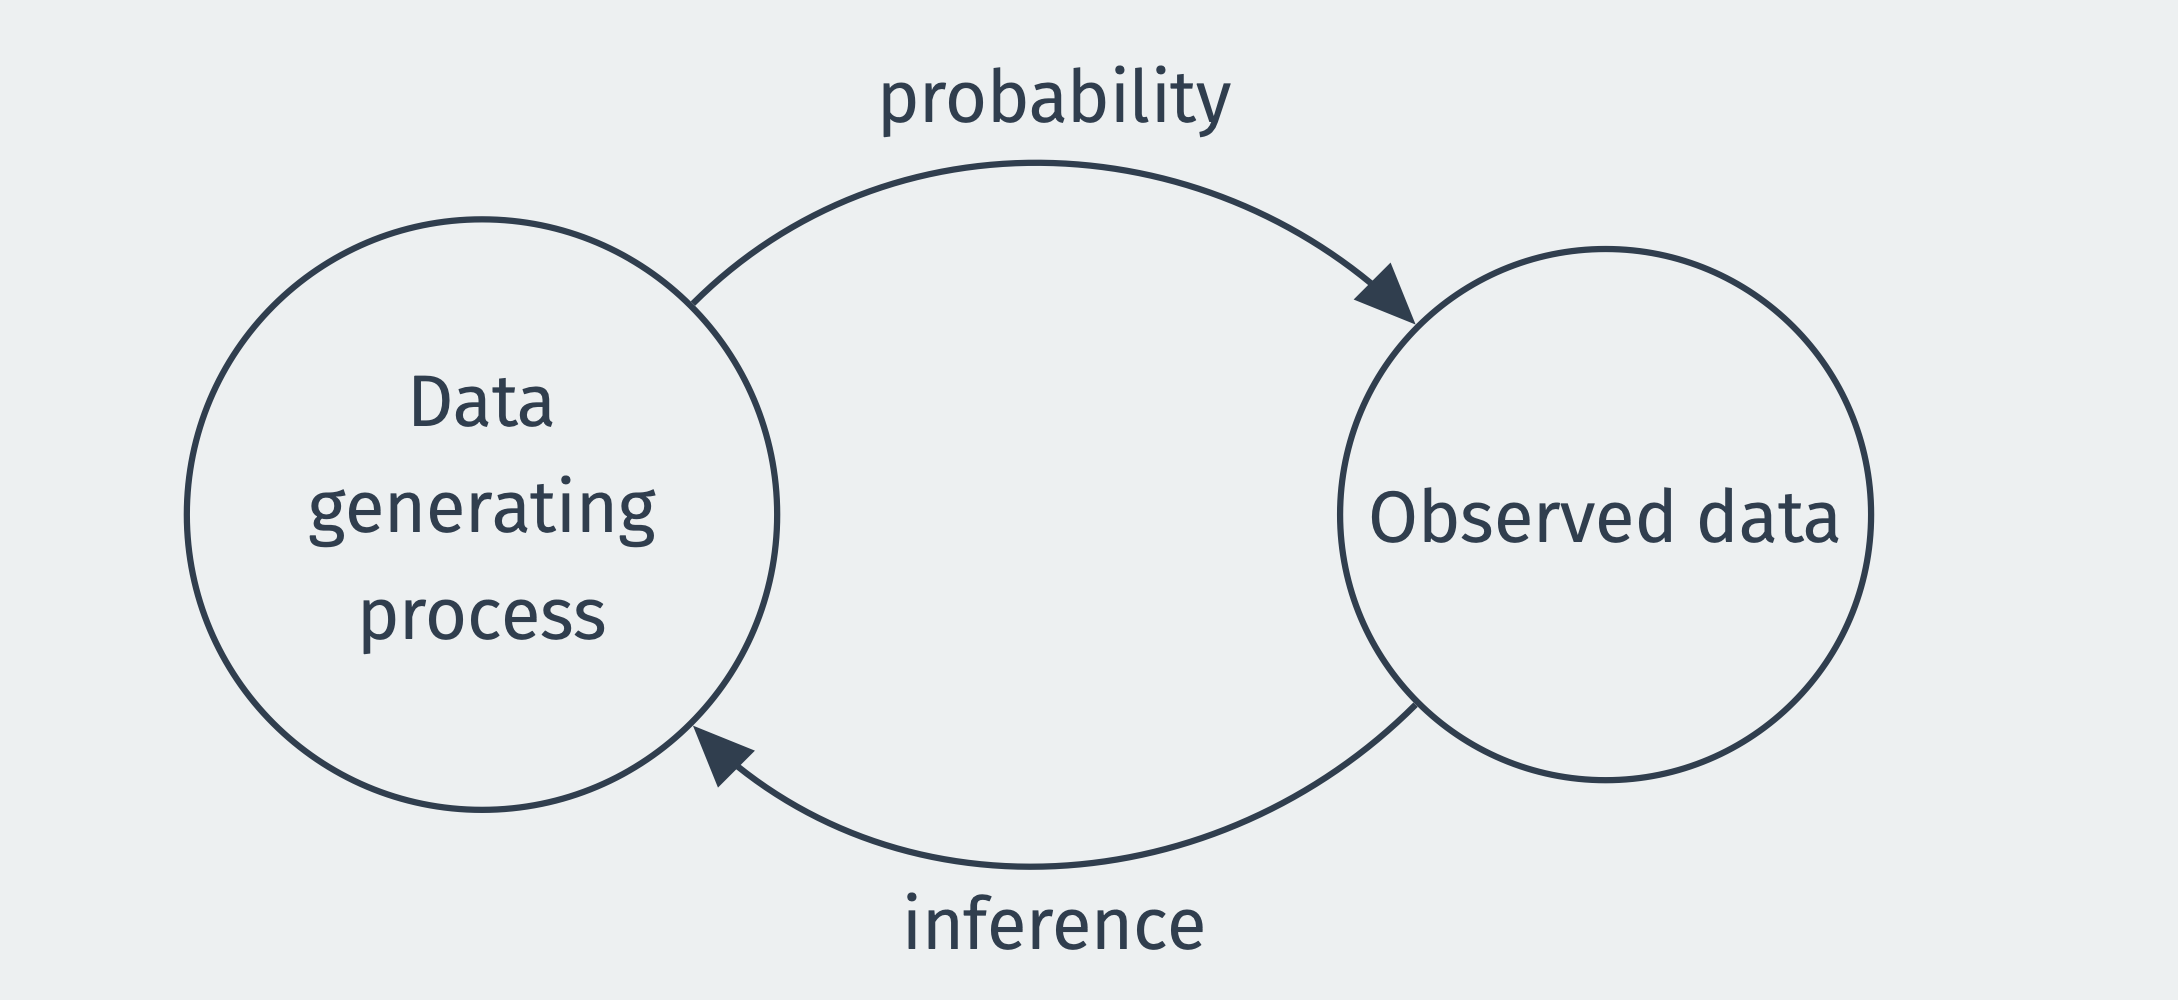
\includegraphics{assets/img/two-direction.png}

An estimator is just a rule for converting our data into a best guess
about some unknown quantity, like the fraction of the public that
supports increasing legal immigration limits. What are the goals of
studying estimators? In short, we prefer to use \textbf{good} estimators
rather than \textbf{bad} estimators. But what makes an estimator good or
bad? You probably have some intuitive sense that, for example, an
estimator that always returns the value 3 is bad. Still, it will be
helpful for us to formally define and explore some properties of
estimators that will allow us to compare them and choose the good over
the bad. We begin with an example that highlights two estimators that,
at first glance, may seem similar.

\begin{example}[Randomized control
trial]\protect\hypertarget{exm-rct}{}\label{exm-rct}

Suppose we are conducting a randomized experiment on framing effects.
All respondents receive some factual information about current levels of
immigration. The message for the treatment group (\(D_i = 1\)) has an
additional framing of the positive benefits of immigration, while the
control group (\(D_i = 0\)) receives no additional framing. The outcome
is a binary outcome on whether the respondent supports increasing legal
immigration limits (\(Y_i = 1\)) or not (\(Y_i = 0\)). The observed data
consists of \(n\) pairs of random variables, the outcome, and the
treatment assignment: \(\{(Y_1, D_1), \ldots, (Y_n, D_n)\}\). Define the
two sample means/proportions in each group as \[
\Ybar_1 = \frac{1}{n_1} \sum_{i: D_i = 1} Y_i, \qquad\qquad \Ybar_0 = \frac{1}{n_0} \sum_{i: D_i = 0} Y_i,
\] where \(n_1 = \sum_{i=1}^n D_i\) is the number of treated units and
\(n_0 = n - n_1\) is the number of control units.

A standard estimator for the treatment effect in a study like this would
be the difference in means, \(\Ybar_1 - \Ybar_0\). But this is only one
possible estimator. We could also estimate the effect by taking this
difference in means separately by party identification and then
averaging those party-specific effects by the size of those groups. This
estimator is commonly called a \textbf{poststratification} estimator,
but it's unclear at first glance which of these two estimators we should
prefer.

\end{example}

We have two goals in this chapter. First, we will introduce the entire
framework of estimation and estimators. We will discuss different ways
to compare the quality of estimators. These are properties that will be
important to any estimator that you will meet now or in the future.
Second, we will establish these properties for a general class of
estimators that can be written as a sample mean. These results are
useful in their own right since these estimators are ubiquitous, but the
derivations also provide examples of how we establish such results.
Building comfort with these proofs will help us understand the arguments
about novel estimators we will inevitably see over the course of our
careers.

\hypertarget{samples-and-populations}{%
\section{Samples and populations}\label{samples-and-populations}}

Let's begin by building a bare-bones probability model for how our data
came to be. We might have a particular data set with a series of numbers
representing the ages, political party affiliations, and opinions of
some survey respondents. But we know that row 58 of our data could have
produced a different set of number if a different respondent had been
selected as row 58 or if that same respondent gave a different opinion
about immigration because they happened to see a news story about it
just before responding. To reason precisely about this type of
uncertainty, we will write \(X_i\) as the random variable representing
the value that row \(i\) of some variable will take, before we see the
data. The distribution of this random variable would tell us what types
of data we should expect to see.

Why do represent the data with random variables when we already know the
value of the data itself? The study of estimation from a frequentist
perspective (which is the perspective of this book) focuses on the
properties of estimators across \textbf{repeated samples}. The random
variable \(X_i\) represents our uncertainty about what value, say, age
will take for respondent \(i\) in any of these samples, and the set
\(\{X_{1}, \ldots, X_{n}\}\) represents our uncertainty about the entire
column of ages for all \(n\) respondents.

For most of this book, we'll focus on a relatively simple setting where
we assume the data \(\{X_1, \ldots, X_n\}\) are \textbf{independent and
identically distributed} (iid) draws from a distribution with cumulative
distribution function (cdf) \(F\). They are independent in that
information about any subset of random variable is not informative about
any other subset of random variables, or, more formally, \[
F_{X_{1},\ldots,X_{n}}(x_{1}, \ldots, x_{n}) = F_{X_{1}}(x_{1})\cdots F_{X_{n}}(x_{n}) = \prod_{i=1}^n F(x_i)
\] where \(F_{X_{1},\ldots,X_{n}}(x_{1}, \ldots, x_{n})\) is the joint
cdf of the random variable and \(F_{X_{j}}(x_{j})\) is the marginal cdf
of the \(j\)th random variable. They are ``identically distributed'' in
the sense that each of the random variables \(X_i\) have the same
marginal distribution, \(F\).

Note that we're being purposely vague about this cdf---it simply
represents the unknown distribution of the data, otherwise known as the
\textbf{data generating process} (DGP). Sometimes \(F\) is also referred
to as the \textbf{population distribution} or even just
\textbf{population}, which has its roots in viewing the data as a random
sample from some larger population.\footnote{This approach to inference
  is often called a \textbf{model-based approach} since we are assuming
  a probability model in the cdf, \(F\). This is usually in contrast to
  a \textbf{design-based approach} to inference that views the
  population of interest as a finite group with fixed traits and the
  only randomness comes from the random sampling procedure.} As a
shorthand, we often say that the collection of random variables
\(\{X_1, \ldots, X_n\}\) is a \textbf{random sample} from population
\(F\) if \(\{X_1, \ldots, X_n\}\) is iid with distribution \(F\). The
\textbf{sample size} \(n\) is the number of units in the sample.

\begin{tcolorbox}[enhanced jigsaw, colbacktitle=quarto-callout-note-color!10!white, colframe=quarto-callout-note-color-frame, arc=.35mm, left=2mm, toptitle=1mm, rightrule=.15mm, title=\textcolor{quarto-callout-note-color}{\faInfo}\hspace{0.5em}{Note}, colback=white, leftrule=.75mm, toprule=.15mm, coltitle=black, opacityback=0, breakable, bottomtitle=1mm, titlerule=0mm, bottomrule=.15mm, opacitybacktitle=0.6]

You might wonder why we reference the distribution of \(X_i\) with the
cdf, \(F\). Mathematical statistics tends to do this to avoid having to
deal with discrete and continuous random variables separately. Every
random variable has a cdf and the cdf contains all information about the
distribution of a random variable.

\end{tcolorbox}

Two metaphors can help build intuition about the concept of viewing the
data as an iid draw from \(F\):

\begin{enumerate}
\def\labelenumi{\arabic{enumi}.}
\tightlist
\item
  \textbf{Random sampling}. Suppose we have a population of size \(N\)
  that is much larger than our sample size \(n\), and we take a random
  sample of size \(n\) from this population with replacement. Then the
  distribution of the data in the random sample will be iid draws from
  the population distribution of the variables we are sampling. For
  instance, suppose we take a random sample from a population of US
  citizens where the population proportion of Democratic party
  identifiers is 0.33. Then if we randomly sample \(n = 100\) US
  citizens, each data point \(X_i\) will be distributed Bernoulli with
  probability of success 0.33.
\item
  \textbf{Groundhog Day}. Random sampling does not always make sense as
  a justification for iid data, especially when the units are not
  samples at all but rather countries, states, or subnational units. In
  this case, we have to appeal to a thought experiment where \(F\)
  represents the fundamental uncertainty in the data-generating process.
  The metaphor here is that if we could re-run history many times, like
  the 1993 American classic comedy \emph{Groundhog Day}, data and
  outcomes would change slightly due to the inherently stochastic nature
  of the world. The iid assumption, then, is that each of the units in
  our data has the same DGP producing this data or the same distribution
  of outcomes under the \emph{Groundhog Day} scenario. The set of all
  these infinite possible draws from the DGP is sometimes referred to as
  the \textbf{superpopulation}.
\end{enumerate}

Note that there are many situations where the iid assumption is not
appropriate. We will cover some of those later in the semester. But much
of the innovation and growth in statistics over the last 50 years has
been figuring out how to perform statistical inference when iid does not
hold. Often, the solutions are specific to the type of iid violation you
have (spatial, time-series, network, or clustered). As a rule of thumb,
though, if you suspect iid is incorrect, your uncertainty statements
will likely be overconfident (for example, confidence intervals, which
we'll cover later, are too small).

Finally, we have introduced the data as a scalar random variable, but
often our data has multiple variables. In that case, we could easily
modify \(X_i\) to be a random vector (that is, a vector of random
variables) and then \(F\) becomes the joint distribution of that random
vector. Nothing substantive changes about the above discussion.

\hypertarget{point-estimation}{%
\section{Point estimation}\label{point-estimation}}

\hypertarget{quantities-of-interest}{%
\subsection{Quantities of interest}\label{quantities-of-interest}}

In statistical inference, our goal is to learn about the data-generating
process. Each data point \(X_i\) represents a draw from a distribution,
captured by the cdf \(F\), and we would like to know more about this
distribution. We might be interested in estimating the cdf at a general
level or only some feature of the distribution, like a mean or
conditional expectation function.

\begin{example}[Population
mean]\protect\hypertarget{exm-prop}{}\label{exm-prop}

Suppose we wanted to know the proportion of US citizens who support
increasing legal immigration in the US, which we denote as \(Y_i = 1\).
Then our quantity of interest is the mean of this random variable,
\(\mu = \E[Y_i] = \P(Y_{i} = 1)\), which is the probability of randomly
drawing someone from the population supporting increased legal
immigration.

\end{example}

\begin{example}[Population
variance]\protect\hypertarget{exm-var}{}\label{exm-var}

Feeling thermometer scores are a prevalent way to assess how a survey
respondent feels about a particular person or group. A survey asks
respondents how warmly they feel about a group from 0 to 100, which we
will denote \(Y_i\). We might be interested in how polarized views are
on a group in the population, and one measure of polarization could be
the variance, or spread, of the distribution of \(Y_i\) around the mean.
In this case, \(\sigma^2 = \V[Y_i]\) would be our quantity of interest.

\end{example}

\begin{example}[RCT
continued]\protect\hypertarget{exm-rct-ii}{}\label{exm-rct-ii}

In Example~\ref{exm-rct}, we discussed a typical estimator for an
experimental study with a binary treatment. The goal of that experiment
is to learn about the difference between two conditional probabilities
(or expectations): the average support for increasing legal immigration
in the treatment group, \(\mu_1 = \E[Y_i \mid D_i = 1]\), and the same
average in the control group, \(\mu_0 = \E[Y_i \mid D_i = 0]\). This
difference, \(\mu_1 - \mu_0\), is a function of unknown features of
these two conditional distributions.

\end{example}

Each of these is a function of the (possibly joint) distribution of the
data, \(F\). In each of these, we are not necessarily interested in the
entire distribution, just summaries of it (central tendency, spread). Of
course, there are situations where we are also interested in the
complete distribution. To be able to speak about estimation in general,
we'll let \(\theta\) represent some generic quantity of interest.
\textbf{Point estimation} describes how we obtain a single ``best
guess'' about \(\theta\).

\begin{tcolorbox}[enhanced jigsaw, colbacktitle=quarto-callout-note-color!10!white, colframe=quarto-callout-note-color-frame, arc=.35mm, left=2mm, toptitle=1mm, rightrule=.15mm, title=\textcolor{quarto-callout-note-color}{\faInfo}\hspace{0.5em}{Note}, colback=white, leftrule=.75mm, toprule=.15mm, coltitle=black, opacityback=0, breakable, bottomtitle=1mm, titlerule=0mm, bottomrule=.15mm, opacitybacktitle=0.6]

Some refer to quantities of interest as \textbf{parameters} or
\textbf{estimands} (that is, the target of estimation).

\end{tcolorbox}

\hypertarget{estimators}{%
\subsection{Estimators}\label{estimators}}

Now that we have a target in mind, we can try to estimate it with our
data. To do so, we first need a rule or algorithm or function that takes
as inputs the data and returns a best guess about the quantity of
interest. One of the most popular and useful algorithm would be to sum
all the data points and divide by the number of points, which we can
write mathematically as \[
\frac{X_1 + X_2 + \cdots + X_n}{n}.
\] This is the much celebrated sample mean, and it provides a rule for
how to take your data and produce a single-number summary of the data.
We might go one pedantic step further and define it as a function of the
data more explicitly, \[
\textsf{mean}(X_1, X_2, \ldots, X_n) = \frac{X_1 + X_2 + \cdots + X_n}{n}.
\] We can use this model to provide a definition for an arbitrary
estimator for an arbitrary quantity of interest.

\begin{definition}[]\protect\hypertarget{def-estimator}{}\label{def-estimator}

An \textbf{estimator} \(\widehat{\theta}_n = \theta(X_1, \ldots, X_n)\)
for some parameter \(\theta\), is a function of the data intended as a
guess about \(\theta\).

\end{definition}

\begin{tcolorbox}[enhanced jigsaw, colbacktitle=quarto-callout-note-color!10!white, colframe=quarto-callout-note-color-frame, arc=.35mm, left=2mm, toptitle=1mm, rightrule=.15mm, title=\textcolor{quarto-callout-note-color}{\faInfo}\hspace{0.5em}{Note}, colback=white, leftrule=.75mm, toprule=.15mm, coltitle=black, opacityback=0, breakable, bottomtitle=1mm, titlerule=0mm, bottomrule=.15mm, opacitybacktitle=0.6]

It is widespread, though not universal, to use the ``hat'' notation to
define an estimator and its estimand. For example, \(\widehat{\theta}\)
(or ``theta hat'') indicates that this estimator is targeting the
parameter \(\theta\).

\end{tcolorbox}

\begin{example}[Estimators for the population
mean]\protect\hypertarget{exm-mean-est}{}\label{exm-mean-est}

Suppose we would like to estimate the population mean of \(F\), which we
will represent as \(\mu = \E[X_i]\). We could choose from several
estimators, all with different properties. \[
\widehat{\theta}_{n,1} = \frac{1}{n} \sum_{i=1}^n X_i, \quad \widehat{\theta}_{n,2} = X_1, \quad \widehat{\theta}_{n,3} = \text{max}(X_1,\ldots,X_n), \quad \widehat{\theta}_{n,4} = 3
\] The first is just the sample mean, which is an intuitive and natural
estimator for the population mean. The second just uses the first
observation. While this seems silly, this is a valid statistic (it's a
function of the data!). The third takes the maximum value in the sample,
and the fourth always returns three, regardless of the data.

\end{example}

When we view the data \(\{X_{1}, \ldots, X_{n}\}\) as a collection of
random variables, then any function of them is also a random variable.
Thus, we can view \(\widehat{\theta}_n\) as a random variable that has a
distribution that induced by the randomness of the sample. Drawing two
different samples of respondents will lead to two different estimates.
For example, here we illustrate two samples of size \(n =5\) from the
population distribution of a binary variable:

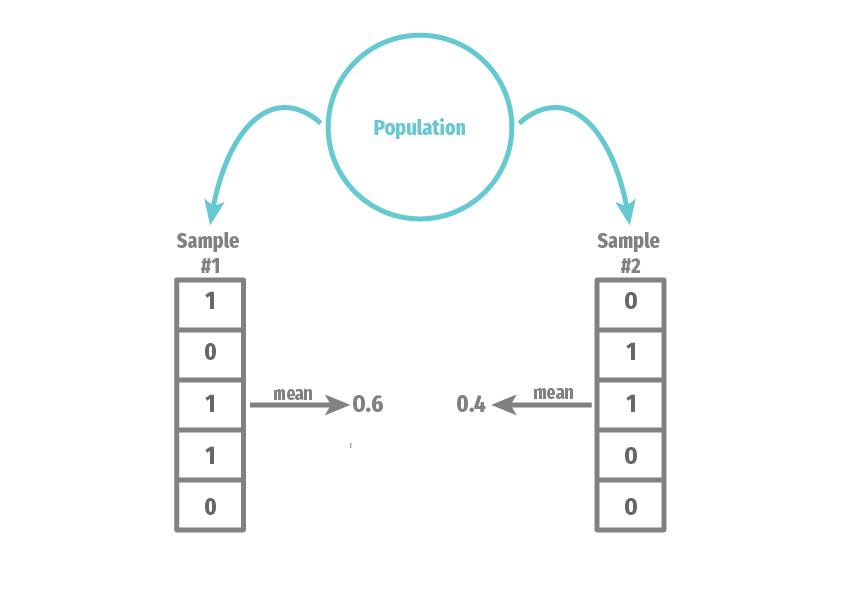
\includegraphics{assets/img/sampling-distribution.png}

We can see that the mean of the variable depends on what exact values
end up in our sample. We refer to the distribution of
\(\widehat{\theta}_n\) across repeated samples as its \textbf{sampling
distribution}. The sampling distribution of an estimator will be the
basis for all of the formal statistical properties of an estimator.

\begin{tcolorbox}[enhanced jigsaw, colbacktitle=quarto-callout-warning-color!10!white, colframe=quarto-callout-warning-color-frame, arc=.35mm, left=2mm, toptitle=1mm, rightrule=.15mm, title=\textcolor{quarto-callout-warning-color}{\faExclamationTriangle}\hspace{0.5em}{Warning}, colback=white, leftrule=.75mm, toprule=.15mm, coltitle=black, opacityback=0, breakable, bottomtitle=1mm, titlerule=0mm, bottomrule=.15mm, opacitybacktitle=0.6]

One important distinction of jargon is between an estimator and an
estimate. The estimator is a function of the data, whereas the
\textbf{estimate} is the \emph{realized value} of the estimator once we
see the data. An estimate is a single number, such as 0.38, that we
calculated in R with our data (our draw from \(F\)). The estimator, on
the other hand, is a random variable that has uncertainty over what
value it will take. Formally, the estimate is
\(\theta(x_1, \ldots, x_n)\) when the data is
\(\{X_1, \ldots, X_n\} = \{x_1, \ldots, x_n\}\), whereas we represent
the estimator as a function of random variables,
\(\widehat{\theta}_n = \theta(X_1, \ldots, X_n)\).

\end{tcolorbox}

\hypertarget{how-to-find-estimators}{%
\section{How to find estimators}\label{how-to-find-estimators}}

Where do estimators come from? This may seem like a question reserved
for statisticians or methodologists or others who are responsible for
``developing new methods.'' But there is value in knowing how estimators
are derived even if we never plan to do that ourselves. In particular,
we can get a sense of the strengths and potential weaknesses of an
estimator if know where it comes from. We will briefly introduce
estimators based on parametric models, before turning to the main focus
of this book, plug-in estimators.

\hypertarget{parametric-models-and-maximum-likelihood}{%
\subsection{Parametric models and maximum
likelihood}\label{parametric-models-and-maximum-likelihood}}

The first method for generating estimators relies on \textbf{parametric
models}, where the researcher specifies the exact distribution (up to
some unknown parameters) of the DGP. Let \(\theta\) be the parameters of
this distribution and we then write \(\{X_1, \ldots, X_n\}\) are iid
draws from \(F_{\theta}\). We should also formally state the set of
possible values the parameters can take, which we call the
\textbf{parameter space} and usually denote as \(\Theta\). Because we're
assuming we know the distribution of the data, we can write the p.d.f.
as \(f(X_i \mid \theta)\) and define the likelihood function as the
product of these p.d.f.s over the units as a function of the parameters:
\[
L(\theta) = \prod_{i=1}^n f(X_i \mid \theta).
\] We can then define the \textbf{maximum likelihood} estimator (MLE)
for \(\theta\) as the values of the parameter that, well, maximize the
likelihood: \[
\widehat{\theta}_{mle} = \argmax_{\theta \in \Theta} \; L(\theta)
\] Sometimes we can use calculus to derive a closed-form expression for
the MLE. Still, we often use iterative techniques that search the
parameter space for the maximum.

Maximum likelihood estimators have very nice properties, especially in
large samples. Unfortunately, they also require the correct knowledge of
the parametric model, which is often difficult to justify. Do we really
know if we should model a given event count variable as Poisson or
Negative Binomial? The attractive properties of MLE are only as good as
our ability to specify the parametric model.

\begin{tcolorbox}[enhanced jigsaw, colbacktitle=quarto-callout-note-color!10!white, colframe=quarto-callout-note-color-frame, arc=.35mm, left=2mm, toptitle=1mm, rightrule=.15mm, title=\textcolor{quarto-callout-note-color}{\faInfo}\hspace{0.5em}{No free lunch}, colback=white, leftrule=.75mm, toprule=.15mm, coltitle=black, opacityback=0, breakable, bottomtitle=1mm, titlerule=0mm, bottomrule=.15mm, opacitybacktitle=0.6]

One essential intuition to build about statistics is the
\textbf{assumptions-precision tradeoff}. You can usually get more
precise estimates if you make stronger and potentially more fragile
assumptions. Conversely, you will almost always get less accurate
estimates if you weaken your assumptions.

\end{tcolorbox}

\hypertarget{plug-in-estimators}{%
\subsection{Plug-in estimators}\label{plug-in-estimators}}

The second broad class of estimators is \textbf{semiparametric} in that
we will specify some finite-dimensional parameters of the DGP but leave
the rest of the distribution unspecified. For example, we might define a
population mean, \(\mu = \E[X_i]\), and a population variance,
\(\sigma^2 = \V[X_i]\) but leave unrestricted the shape of the
distribution. This approach ensures that our estimators will be less
dependent on correctly specifying distributions we have little intuition
about.

The primary method for constructing estimators in this setting is to use
the \textbf{plug-in estimator}, or the estimator that replaces any
population mean with a sample mean. Obviously, in the case of estimating
the population mean, \(\mu\), this means we will use the \textbf{sample
mean} as its estimate: \[
\Xbar_n = \frac{1}{n} \sum_{i=1}^n X_i \quad \text{estimates} \quad \E[X_i] = \int_{\mathcal{X}} x f(x)dx
\] What are we doing here? We are replacing the unknown population
distribution \(f(x)\) in the population mean with a discrete uniform
distribution over our data points, with \(1/n\) probability assigned to
each unit. Why do this? It encodes that if we have a random sample, our
best guess about the population distribution of \(X_i\) is the sample
distribution in our actual data. If this intuition fails, you can hold
onto an analog principle: sample means of random variables are natural
estimators of population means.

What about estimating something more complicated, like the expected
value of a function of the data, \(\theta = \E[r(X_i)]\)? The key is to
see that \(f(X_i)\) is also a random variable. Let's call this random
variable \(Y_i = f(X_i)\). Now we can see that \(\theta\) is just the
population expectation of this random variable, and using the plug-in
estimator, we get: \[
\widehat{\theta} = \frac{1}{n} \sum_{i=1}^n Y_i = \frac{1}{n} \sum_{i=1}^n r(X_i). 
\]

With these facts in hand, we can describe the more general plug-in
estimator. When we want to estimate some quantity of interest that is a
function of population means, we can generate a plug-in estimator by
replacing any population mean with a sample mean. Formally, let
\(\alpha = g\left(\E[r(X_i)]\right)\) be a parameter that is defined as
a function of the population mean of a (possibly vector-valued) function
of the data. Then, we can estimate this parameter by plugging in the
sample mean for the population mean to get the \textbf{plug-in
estimator}, \[
\widehat{\alpha} = g\left( \frac{1}{n} \sum_{i=1}^n r(X_i) \right) \quad \text{estimates} \quad \alpha = g\left(\E[r(X_i)]\right)
\] This approach to plug-in estimation with sample means is very general
and will allow us to derive estimators in various settings.

\begin{example}[Estimating population
variance]\protect\hypertarget{exm-var-est}{}\label{exm-var-est}

The population variance of a random variable is
\(\sigma^2 = \E[(X_i - \E[X_i])^2]\). To derive a plug-in estimator for
this quantity, we replace the inner \(\E[X_i]\) with \(\Xbar_n\) and the
outer expectation with another sample mean: \[
\widehat{\sigma}^2 = \frac{1}{n} \sum_{i=1}^n (X_i - \Xbar_n)^2.
\] This plug-in estimator differs from the standard sample variance,
which divides by \(n - 1\) rather than \(n\). This minor difference does
not matter in moderate to large samples.

\end{example}

\begin{example}[Estimating population
covariance]\protect\hypertarget{exm-cov-est}{}\label{exm-cov-est}

Suppose we have two variables, \((X_i, Y_i)\). A natural quantity of
interest here is the population covariance between these variables, \[
\sigma_{xy} = \text{Cov}[X_i,Y_i] = \E[(X_i - \E[X_i])(Y_i-\E[Y_i])],
\] which has the plug-in estimator, \[
\widehat{\sigma}_{xy} = \frac{1}{n} \sum_{i=1}^n (X_i - \Xbar_n)(Y_i - \Ybar_n).
\]

\end{example}

\begin{tcolorbox}[enhanced jigsaw, colbacktitle=quarto-callout-note-color!10!white, colframe=quarto-callout-note-color-frame, arc=.35mm, left=2mm, toptitle=1mm, rightrule=.15mm, title=\textcolor{quarto-callout-note-color}{\faInfo}\hspace{0.5em}{Notation alert}, colback=white, leftrule=.75mm, toprule=.15mm, coltitle=black, opacityback=0, breakable, bottomtitle=1mm, titlerule=0mm, bottomrule=.15mm, opacitybacktitle=0.6]

Given the connection between the population mean and the sample mean,
you will sometimes see the \(\E_n[\cdot]\) operator used as a shorthand
for the sample average: \[
\E_n[r(X_i)] \equiv \frac{1}{n} \sum_{i=1}^n r(X_i).
\]

\end{tcolorbox}

Finally, plug-in estimation goes beyond just replacing population means
with sample means. We can derive estimators of the population quantiles
like the median with sample versions of those quantities. What unifies
all of these approaches is replacing the unknown population cdf, \(F\),
with the empirical cdf, \[
\widehat{F}_n(x) = \frac{\sum_{i=1}^n \mathbb{I}(X_i \leq x)}{n},
\] where \(\mathbb{I}(A)\) is an \emph{indicator function} that take the
value 1 if the event \(A\) occurs and 0 otherwise. For a more complete
and technical treatment of these ideas, see Wasserman (2004) Chapter 7.

\hypertarget{the-three-distributions-population-empirical-and-sampling}{%
\section{The three distributions: population, empirical, and
sampling}\label{the-three-distributions-population-empirical-and-sampling}}

Once we start to wade into estimation, there are several distributions
to keep track of, and things can quickly become confusing. Three
specific distributions are all related and easy to confuse, but keeping
them distinct is crucial.

The \textbf{population distribution} is the distribution of the random
variable, \(X_i\), which we have labeled \(F\) and is our target of
inference. Then there is the \textbf{empirical distribution}, which is
the distribution of the actual realizations of the random variables in
our samples (that is, the numbers in our data frame),
\(X_1, \ldots, X_n\). Because this is a random sample from the
population distribution and can serve as an estimator of \(F\), we
sometimes call this \(\widehat{F}_n\).

Separately from both is the \textbf{sampling distribution of an
estimator}, which is the probability distribution of
\(\widehat{\theta}_n\). It represents our uncertainty about our estimate
before we see the data. Remember that our estimator is itself a random
variable because it is a function of random variables: the data itself.
That is, we defined the estimator as
\(\widehat{\theta}_n = \theta(X_1, \ldots, X_n)\).

\begin{example}[Likert
responses]\protect\hypertarget{exm-three-dist}{}\label{exm-three-dist}

Suppose \(X_i\) is the answer to a question, ``How much do you agree
with the following statement: Immigrants are a net positive for the
United States,'' with a \(X_i = 0\) being ``strongly disagree,''
\(X_i = 1\) being ``disagree,'' \(X_i = 2\) being ``neither agree nor
disagree,'' \(X_i = 3\) being ``agree,'' and \(X_i = 4\) being
``strongly agree.''

The population distribution describes the probability of randomly
selecting a person with each one of these values, \(\P(X_i = x)\). The
empirical distribution would be the fraction of our data taking each
value. And the sampling distribution of the sample mean, \(\Xbar_n\),
would be the distribution of the sample mean across repeated samples
from the population.

Suppose the population distribution was binomial with four trials and
probability of success \(p = 0.4\). We could generate one sample with
\(n = 10\) and thus one empirical distribution using \texttt{rbinom()}:

\begin{Shaded}
\begin{Highlighting}[]
\NormalTok{my\_samp }\OtherTok{\textless{}{-}} \FunctionTok{rbinom}\NormalTok{(}\AttributeTok{n =} \DecValTok{10}\NormalTok{, }\AttributeTok{size =} \DecValTok{5}\NormalTok{, }\AttributeTok{prob =} \FloatTok{0.4}\NormalTok{)}
\NormalTok{my\_samp}
\end{Highlighting}
\end{Shaded}

\begin{verbatim}
 [1] 1 3 2 3 4 0 2 3 2 2
\end{verbatim}

\begin{Shaded}
\begin{Highlighting}[]
\FunctionTok{table}\NormalTok{(my\_samp)}
\end{Highlighting}
\end{Shaded}

\begin{verbatim}
my_samp
0 1 2 3 4 
1 1 4 3 1 
\end{verbatim}

And we can generate one draw from the sampling distribution of
\(\Xbar_n\) by taking the mean of this sample:

\begin{Shaded}
\begin{Highlighting}[]
\FunctionTok{mean}\NormalTok{(my\_samp)}
\end{Highlighting}
\end{Shaded}

\begin{verbatim}
[1] 2.2
\end{verbatim}

But, if we had a different sample, it would have a different empirical
distribution and thus give us a different estimate of the sample mean:

\begin{Shaded}
\begin{Highlighting}[]
\NormalTok{my\_samp2 }\OtherTok{\textless{}{-}} \FunctionTok{rbinom}\NormalTok{(}\AttributeTok{n =} \DecValTok{10}\NormalTok{, }\AttributeTok{size =} \DecValTok{5}\NormalTok{, }\AttributeTok{prob =} \FloatTok{0.4}\NormalTok{)}
\FunctionTok{mean}\NormalTok{(my\_samp2) }
\end{Highlighting}
\end{Shaded}

\begin{verbatim}
[1] 2
\end{verbatim}

The sampling distribution is the distribution of these sample means
across repeated sampling.

\end{example}

\hypertarget{finite-sample-properties-of-estimators}{%
\section{Finite-sample properties of
estimators}\label{finite-sample-properties-of-estimators}}

As we discussed when we introduced estimators, their usefulness depends
on how well they help us learn about the quantity of interest. If we get
an estimate \(\widehat{\theta} = 1.6\), we would like to know that this
is ``close'' to the true parameter \(\theta\). The sampling distribution
is the key to answering these questions. Intuitively, we would like the
sampling distribution of \(\widehat{\theta}_n\) to be as tightly
clustered around the true as \(\theta\) as possible. Here, though, we
run into a problem: the sampling distribution depends on the population
distribution since it is about repeated samples of the data from that
distribution filtered through the function \(\theta()\). Since \(F\) is
unknown, this implies that the sampling distribution will also usually
be unknown.

Even though we cannot precisely pin down the entire sampling
distribution, we can use assumptions to derive specific properties of
the sampling distribution that will be useful in comparing estimators.

\hypertarget{bias}{%
\subsection{Bias}\label{bias}}

The first property of the sampling distribution concerns its central
tendency. In particular, we will define the \textbf{bias} (or
\textbf{estimation bias}) of estimator \(\widehat{\theta}\) for
parameter \(\theta\) as \[
\text{bias}[\widehat{\theta}] = \E[\widehat{\theta}] - \theta,
\] which is the difference between the mean of the estimator (across
repeated samples) and the true parameter. All else equal, we would like
estimation bias to be as small as possible. The smallest possible bias,
obviously, is 0, and we define an \textbf{unbiased estimator} as one
with \(\text{bias}[\widehat{\theta}] = 0\) or equivalently,
\(\E[\widehat{\theta}] = \theta\).

However, all else is not always equal, and unbiasedness is not a
property to become overly attached to. Many biased estimators have other
attractive properties, and many popular modern estimators are biased.

\begin{example}[Unbiasedness of the sample
mean]\protect\hypertarget{exm-mean-unbiased}{}\label{exm-mean-unbiased}

We can show that the sample mean is unbiased for the population mean
when the data is iid and \(\E|X| < \infty\). In particular, we simply
apply the rules of expectations: \[\begin{aligned}
\E\left[ \Xbar_n \right] &= \E\left[\frac{1}{n} \sum_{i=1}^n X_i\right] & (\text{definition of } \Xbar_n) \\
&= \frac{1}{n} \sum_{i=1}^n \E[X_i] & (\text{linearity of } \E)\\
&= \frac{1}{n} \sum_{i=1}^n \mu & (X_i \text{ identically distributed})\\
&= \mu.
\end{aligned}\] Notice that we only used the ``identically distributed''
part of iid. Independence is not needed.

\end{example}

\begin{tcolorbox}[enhanced jigsaw, colbacktitle=quarto-callout-warning-color!10!white, colframe=quarto-callout-warning-color-frame, arc=.35mm, left=2mm, toptitle=1mm, rightrule=.15mm, title=\textcolor{quarto-callout-warning-color}{\faExclamationTriangle}\hspace{0.5em}{Warning}, colback=white, leftrule=.75mm, toprule=.15mm, coltitle=black, opacityback=0, breakable, bottomtitle=1mm, titlerule=0mm, bottomrule=.15mm, opacitybacktitle=0.6]

Properties like unbiasedness might only hold for a subset of DGPs. For
example, we just showed that the sample mean is unbiased, but only when
the population mean is finite. There are probability distributions like
the Cauchy where the expected value diverges and is not finite. So we
are dealing with a restricted class of DGPs that rules out such
distributions. You may see this sometimes formalized by defining a class
\(\mathcal{F}\) of distributions, and unbiasedness might hold in that
class if it is unbiased for all \(F \in \mathcal{F}\).

\end{tcolorbox}

\hypertarget{estimation-variance-and-the-standard-error}{%
\subsection{Estimation variance and the standard
error}\label{estimation-variance-and-the-standard-error}}

If a ``good'' estimator tends to be close to the truth, we should also
care about the spread of the sampling distribution. In particular, we
define the \textbf{sampling variance} as the variance of an estimator's
sampling distribution, \(\V[\widehat{\theta}]\), which measures how
spread out the estimator is around its mean. For an unbiased estimator,
lower sampling variance implies the distribution of \(\widehat{\theta}\)
is more concentrated around the truth.

\begin{example}[Sampling variance of the sample
mean]\protect\hypertarget{exm-mean-var}{}\label{exm-mean-var}

We can establish the sampling variance of the sample mean of iid data
for all \(F\) such that \(\V[X_i]\) is finite (more precisely,
\(\E[X_i^2] < \infty\))

\[\begin{aligned}
  \V\left[ \Xbar_n \right] &= \V\left[ \frac{1}{n} \sum_{i=1}^n X_i \right] & (\text{definition of } \Xbar_n) \\
                           &= \frac{1}{n^2} \V\left[ \sum_{i=1}^n X_i \right] & (\text{property of } \V) \\
                           &= \frac{1}{n^2} \sum_{i=1}^n \V[X_i] & (\text{independence}) \\
                           &= \frac{1}{n^2} \sum_{i=1}^n \sigma^2 & (X_i \text{ identically distributed}) \\
                           &= \frac{\sigma^2}{n}
\end{aligned}\]

\end{example}

An alternative measure of spread for any distribution is the standard
deviation, which is on the same scale as the original random variable.
We call the standard deviation of the sampling distribution of
\(\widehat{\theta}\) the \textbf{standard error} of
\(\widehat{\theta}\):
\(\se(\widehat{\theta}) = \sqrt{\V[\widehat{\theta}]}\).

Given the above derivation, the standard error of the sample mean under
iid sampling is \(\sigma / \sqrt{n}\).

\hypertarget{mean-squared-error}{%
\subsection{Mean squared error}\label{mean-squared-error}}

Bias and sampling variance measure two different aspects of being a
``good'' estimator. Ideally, we want the estimator to be as close as
possible to the true value. One summary measure of the quality of an
estimator is the \textbf{mean squared error} or \textbf{MSE}, which is\\
\[
\text{MSE} = \E[(\widehat{\theta}_n-\theta)^2].
\] Ideally, we would have this be as small as possible!

We can also relate the MSE to the bias and the sampling variance
(provided it is finite) with the following decomposition result: \[
\text{MSE} = \text{bias}[\widehat{\theta}_n]^2 + \V[\widehat{\theta}_n]
\] This decomposition implies that, for unbiased estimators, MSE is the
sampling variance. It also highlights why we might accept some bias for
significant reductions in variance for lower overall MSE.

\begin{figure}

{\centering 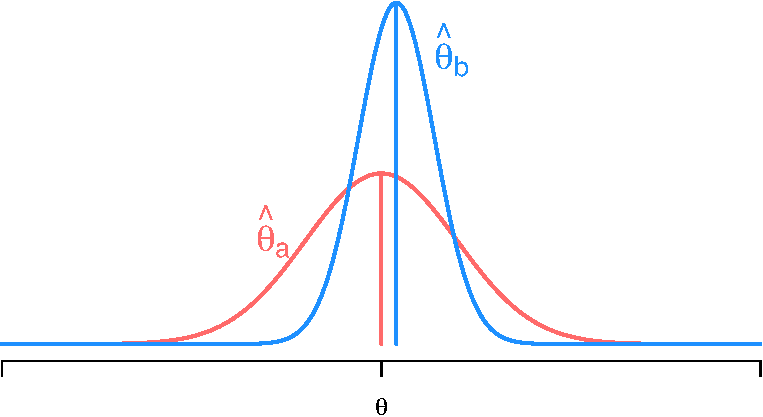
\includegraphics{02_estimation_files/figure-pdf/mse-1.pdf}

}

\caption{Two sampling distributions}

\end{figure}

In this figure, we show the sampling distributions of two estimators,
\(\widehat{\theta}_a\), which is unbiased (centered on the true value
\(\theta\)) but with a high sampling variance, and
\(\widehat{\theta}_b\) which is slightly biased but with much lower
sampling variance. Even though \(\widehat{\theta}_b\) is biased, the
probability of drawing a value close to the truth is higher than for
\(\widehat{\theta}_a\). This balancing between bias and variance is
precisely what the MSE helps capture and, indeed, in this case,
\(MSE[\widehat{\theta}_b] < MSE[\widehat{\theta}_a]\).

\hypertarget{sec-asymptotics}{%
\chapter{Asymptotics}\label{sec-asymptotics}}

\hypertarget{introduction-2}{%
\section{Introduction}\label{introduction-2}}

In the last chapter, we defined estimators and started investigating
their finite-sample properties like unbiasedness and the sampling
variance. We call these ``finite-sample'' properties since they hold at
any sample size. We saw that under iid data, the sample mean is unbiased
for the population mean, but this result holds as much for \(n = 10\) as
it does for \(n = 1,000,000\). But these properties are also of limited
use: we only learn the center and spread of the sampling distribution of
\(\Xbar_n\) from these results. What about the shape of the
distribution? We can often derive the shape if we are willing to make
certain assumptions on the underlying data (for example, if the data is
normal, then the sample means will also be normal). Still, this approach
is brittle: if our parametric assumption is false, we're back to square
one.

In this chapter, we will take a different approach and see what happens
to the sampling distribution of estimators as the sample size gets
large, which we refer to as \textbf{asymptotic theory}. While
asymptotics will often simplify our derivations, it is essential to
understand everything we do with asymptotics will be an approximation.
No one ever has infinite data, but we hope that the approximations will
be closer to the truth as our samples get larger.

\hypertarget{why-convergence-with-probability-is-hard}{%
\section{Why convergence with probability is
hard}\label{why-convergence-with-probability-is-hard}}

It's helpful to review the basic idea of convergence in deterministic
sequences from calculus:

\begin{definition}[]\protect\hypertarget{def-limit}{}\label{def-limit}

A sequence \(\{a_n: n = 1, 2, \ldots\}\) has the \textbf{limit} \(a\)
written \(a_n \rightarrow a\) as \(n\rightarrow \infty\) or
\(\lim_{n\rightarrow \infty} a_n = a\) if for all \(\epsilon > 0\) there
is some \(n_{\epsilon} < \infty\) such that for all
\(n \geq n_{\epsilon}\), \(|a_n - a| \leq \epsilon\).

\end{definition}

We say that \(a_n\) \textbf{converges} to \(a\) if
\(\lim_{n\rightarrow\infty} a_n = a\). Basically, a sequence converges
to a number if the sequence gets closer and closer to that number as the
sequence goes on.

Can we apply this same idea to sequences of random variables (like
estimators)? Let's look at a few examples that help clarify why this
might be difficult.\footnote{Due to Wasserman (2004), Chapter 5.} Let's
say that we have a sequence of \(a_n = a\) for all \(n\) (that is, a
constant sequence). Then obviously
\(\lim_{n\rightarrow\infty} a_n = a\). Now let's say we have a sequence
of random variables, \(X_1, X_2, \ldots\), that are all independent with
a standard normal distribution, \(N(0,1)\). From the analogy to the
deterministic case, it is tempting to say that \(X_n\) converges to
\(X \sim N(0, 1)\), but notice that because they are all different
random variables, \(\P(X_n = X) = 0\). Thus, we must be careful about
saying how one variable converges to another variable.

Another example highlights subtle problems with a sequence of random
variables converging to a single value. Suppose we have a sequence of
random variables \(X_1, X_2, \ldots\) where \(X_n \sim N(0, 1/n)\).
Clearly, the distribution of \(X_n\) will concentrate around 0 for large
values of \(n\), so it is tempting to say that \(X_n\) converges to 0.
But notice that \(\P(X_n = 0) = 0\) because of the nature of continuous
random variables.

\hypertarget{convergence-in-probability-and-consistency}{%
\section{Convergence in probability and
consistency}\label{convergence-in-probability-and-consistency}}

There are several different ways that a sequence of random variance can
converge. The first type of convergence deals with sequences converging
to a single value.\footnote{Technically, a sequence can also converge in
  probability to another random variable, but the use case of converging
  to a single number is much more common in evaluating estimators.}

\begin{definition}[]\protect\hypertarget{def-inprob}{}\label{def-inprob}

A sequence of random variables, \(X_1, X_2, \ldots\), is said to
\textbf{converge in probability} to a value \(b\) if for every
\(\varepsilon > 0\), \[
\P(|X_n - b| > \varepsilon) \rightarrow 0,
\] as \(n\rightarrow \infty\). We write this \(X_n \inprob b\).

\end{definition}

With deterministic sequences, we said that \(a_n\) converges to \(a\) as
it gets closer and closer to \(a\) as \(n\) gets bigger. For convergence
in probability, the sequence of random variables converges to \(b\) if
the probability that random variables are far away from \(b\) gets
smaller and smaller as \(n\) gets big.

\begin{tcolorbox}[enhanced jigsaw, colbacktitle=quarto-callout-note-color!10!white, colframe=quarto-callout-note-color-frame, arc=.35mm, left=2mm, toptitle=1mm, rightrule=.15mm, title=\textcolor{quarto-callout-note-color}{\faInfo}\hspace{0.5em}{Notation alert}, colback=white, leftrule=.75mm, toprule=.15mm, coltitle=black, opacityback=0, breakable, bottomtitle=1mm, titlerule=0mm, bottomrule=.15mm, opacitybacktitle=0.6]

You will sometimes see convergence in probability written as
\(\text{plim}(Z_n) = b\) if \(Z_n \inprob b\), \(\text{plim}\) stands
for ``probability limit.''

\end{tcolorbox}

Convergence in probability is crucial for evaluating estimators. While
we said that unbiasedness was not the be-all and end-all of properties
of estimators, the following property is an essential and fundamental
property that we would like all good estimators to have.

\begin{definition}[]\protect\hypertarget{def-consistency}{}\label{def-consistency}

An estimator is \textbf{consistent} if
\(\widehat{\theta}_n \inprob \theta\).

\end{definition}

Consistency of an estimator implies that the sampling distribution of
this estimator ``collapses'' on the true value as the sample size gets
large. We say an estimator is inconsistent if it converges in
probability to any other value, which is obviously a terrible property
of an estimator. As the sample size gets large, the probability that an
inconsistent estimator will be close to the truth will approach 0.

We can also define convergence in probability for a sequence of random
vectors, \(\X_1, \X_2, \ldots\), where
\(\X_i = (X_{i1}, \ldots, X_{ik})\) is a random vector of length \(k\).
This sequence convergences in probability to a vector
\(\mb{b} = (b_1, \ldots, b_k)\) if and only if each random variable in
the vector converges to the corresponding element in \(\mb{b}\), or that
\(X_{nj} \inprob b_j\) for all \(j = 1, \ldots, k\).

\hypertarget{useful-inequalities}{%
\section{Useful inequalities}\label{useful-inequalities}}

At first glance, establishing an estimator's consistency will be
difficult. How can we know if a distribution will collapse to a specific
value without knowing the shape or family of the distribution? It turns
out that there are certain relationships between the mean and variance
of a random variable and certain probability statements that hold for
all distributions (that have finite variance, at least). These
relationships will be crucial to establishing results that do not depend
on a specific distribution.

\begin{theorem}[Markov
Inequality]\protect\hypertarget{thm-markov}{}\label{thm-markov}

For any r.v. \(X\) and any \(\delta >0\), \[
\P(|X| \geq \delta) \leq \frac{\E[|X|]}{\delta}.
\]

\end{theorem}

\begin{proof}

Notice that we can let \(Y = |X|/\delta\) and rewrite the statement as
\(\P(Y \geq 1) \leq \E[Y]\) (since \(\E[|X|]/\delta = \E[|X|/\delta]\)
by the properties of expectation), which is what we will show. But
notice that \[
\mathbb{I}(Y \geq 1) \leq Y.
\] Why does this hold? We can investigate the two possible values of the
indicator function to see. If \(Y\) is less than 1, then the indicator
function will be 0, but recall that \(Y\) is nonnegative, so we know
that it must be at least as big as 0 so that inequality holds. If
\(Y \geq 1\), then the indicator function will take the value one, but
we just said that \(Y \geq 1\), so the inequality holds. If we take the
expectation of both sides of this inequality, we obtain the result
(remember, the expectation of an indicator function is the probability
of the event).

\end{proof}

In words, Markov's inequality says that the probability of a random
variable being large in magnitude cannot be high if the average is not
large in magnitude. Blitzstein and Hwang (2019) provide an excellent
intuition behind this result. Let \(X\) be the income of a randomly
selected individual in a population and set \(\delta = 2\E[X]\) so that
the inequality becomes \(\P(X > 2\E[X]) < 1/2\) (assuming that all
income is nonnegative). Here, the inequality says that the share of the
population with an income twice the average must be less than 0.5 since
if more than half the population were making twice the average income,
then the average would have to be higher.

It's pretty astounding how general this result is since it holds for all
random variables. Of course, its generality comes at the expense of not
being very informative. If \(\E[|X|] = 5\), for instance, the inequality
tells us that \(\P(|X| \geq 1) \leq 5\), which is not very helpful since
we already know that probabilities are less than 1! We can get tighter
bounds if we are willing to make some assumptions about \(X\).

\begin{theorem}[Chebyshev
Inequality]\protect\hypertarget{thm-chebyshev}{}\label{thm-chebyshev}

Suppose that \(X\) is r.v. for which \(\V[X] < \infty\). Then, for every
real number \(\delta > 0\), \[
\P(|X-\E[X]| \geq \delta) \leq \frac{\V[X]}{\delta^2}.
\]

\end{theorem}

\begin{proof}

To prove this, we only need to square both sides of the inequality
inside the probability statement and apply Markov's inequality: \[
\P\left( |X - \E[X]| \geq \delta \right) = \P((X-\E[X])^2 \geq \delta^2) \leq \frac{\E[(X - \E[X])^2]}{\delta^2} = \frac{\V[X]}{\delta^2},
\] with the last equality holding by the definition of variance.

\end{proof}

Chebyshev's inequality is a straightforward extension of the Markov
result: the probability of a random variable being far from its mean
(that is, \(|X-\E[X]|\) being large) is limited by the variance of the
random variable. If we let \(\delta = c\sigma\), where \(\sigma\) is the
standard deviation of \(X\), then we can use this result to bound the
normalized: \[
\P\left(\frac{|X - \E[X]|}{\sigma} > c \right) \leq \frac{1}{c^2}.
\] This statement says the probability of being two standard deviations
away from the mean must be less than 1/4 = 0.25. Notice that this bound
can be fairly wide. If \(X\) has a normal distribution, we know that
about 5\% of draws will be greater than 2 SDs away from the mean, much
lower than the 25\% bound implied by Chebyshev's inequality.

\hypertarget{the-law-of-large-numbers}{%
\section{The law of large numbers}\label{the-law-of-large-numbers}}

We can now use these inequalities to show how estimators can be
consistent for their target quantities of interest. Why are these
inequalities helpful for this purpose? Remember that convergence in
probability was about the probability of an estimator being far away
from a value going to zero. Chebyshev's inequality shows that we can
bound these exact probabilities.

The most famous consistency result has a special name.

\begin{theorem}[Weak Law of Large
Numbers]\protect\hypertarget{thm-lln}{}\label{thm-lln}

Let \(X_1, \ldots, X_n\) be i.i.d. draws from a distribution with mean
\(\mu = \E[X_i]\) and variance \(\sigma^2 = \V[X_i] < \infty\). Let
\(\Xbar_n = \frac{1}{n} \sum_{i =1}^n X_i\). Then,
\(\Xbar_n \inprob \mu\).

\end{theorem}

\begin{proof}

Recall that the sample mean is unbiased, so \(\E[\Xbar_n] = \mu\) with
sampling variance \(\sigma^2/n\). We can then apply Chebyshev to the
sample mean to get \[
\P(|\Xbar_n - \mu| \geq \delta) \leq \frac{\sigma^2}{n\delta^2}
\] An \(n\rightarrow\infty\), the right-hand side goes to 0, which means
that the left-hand side also must go to 0, which is the definition of
\(\Xbar_n\) converging in probability to \(\mu\).

\end{proof}

The weak law of large numbers (WLLN) shows that, under general
conditions, the sample mean gets closer to the population mean as
\(n\rightarrow\infty\). This result holds even when the variance of the
data is infinite, though that's a situation that most analysts will
rarely face.

\begin{tcolorbox}[enhanced jigsaw, colbacktitle=quarto-callout-note-color!10!white, colframe=quarto-callout-note-color-frame, arc=.35mm, left=2mm, toptitle=1mm, rightrule=.15mm, title=\textcolor{quarto-callout-note-color}{\faInfo}\hspace{0.5em}{Note}, colback=white, leftrule=.75mm, toprule=.15mm, coltitle=black, opacityback=0, breakable, bottomtitle=1mm, titlerule=0mm, bottomrule=.15mm, opacitybacktitle=0.6]

The naming of the ``weak'' law of large numbers seems to imply the
existence of a ``strong'' law of large numbers (SLLN), and this is true.
The SLLN states that the sample mean converges to the population mean
with probability 1. This type of convergence, called \textbf{almost sure
convergence}, is stronger than convergence in probability which only
says that the probability of the sample mean being close to the
population mean converges to 1. While it is nice to know that this
stronger form of convergence holds for the sample mean under the same
assumptions, it is rare for folks outside of theoretical probability and
statistics to rely on almost sure convergence.

\end{tcolorbox}

\begin{example}[]\protect\hypertarget{exm-lln}{}\label{exm-lln}

It can be helpful to see how the distribution of the sample mean changes
as a function of the sample size to appreciate the WLLN. We can show
this by taking repeated iid samples of different sizes from an
exponential random variable with rate parameter 0.5 so that
\(\E[X_i] = 2\). In Figure~\ref{fig-lln-sim}, we show the distribution
of the sample mean (across repeated samples) when the sample size is 15
(black), 30 (violet), 100 (blue), and 1000 (green). We can see how the
sample mean distribution is ``collapsing'' on the true population mean,
2. The probability of being far away from 2 becomes progressively
smaller.

\begin{figure}

{\centering 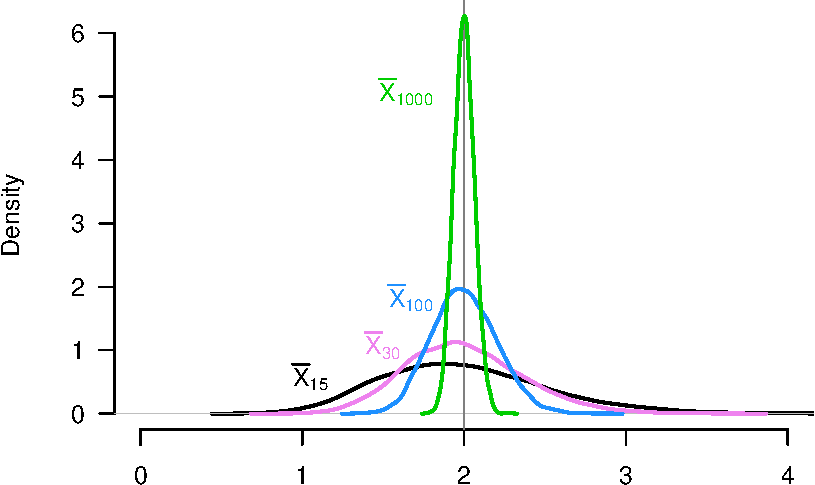
\includegraphics{03_asymptotics_files/figure-pdf/fig-lln-sim-1.pdf}

}

\caption{\label{fig-lln-sim}Sampling distribution of the sample mean as
a function of sample size.}

\end{figure}

\end{example}

The WLLN also holds for random vectors in addition to random variables.
Let \((\X_1, \ldots, \X_n)\) be an iid sample of random vectors of
length \(k\), \(\mb{X}_i = (X_{i1}, \ldots, X_{ik})\). We can define the
vector sample mean as just the vector of sample means for each of the
entries:

\[
\overline{\mb{X}}_n = \frac{1}{n} \sum_{i=1}^n \mb{X}_i =
\begin{pmatrix}
\Xbar_{n,1} \\ \Xbar_{n,2} \\ \vdots \\ \Xbar_{n, k}
\end{pmatrix}
\] Since this is just a vector of sample means, each random variable in
the random vector will converge in probability to the mean of that
random variable. Fortunately, this is the exact definition of
convergence in probability for random vectors. We formally write this in
the following theorem.

\begin{theorem}[]\protect\hypertarget{thm-vector-wlln}{}\label{thm-vector-wlln}

If \(\X_i \in \mathbb{R}^k\) are iid draws from a distribution with
\(\E[X_{ij}] < \infty\) for all \(j=1,\ldots,k\) then as
\(n\rightarrow\infty\)

\[
\overline{\mb{X}}_n \inprob \E[\X] =
\begin{pmatrix}
\E[X_{i1}] \\ \E[X_{i2}] \\ \vdots \\ \E[X_{ik}]
\end{pmatrix}.
\]

\end{theorem}

\begin{tcolorbox}[enhanced jigsaw, colbacktitle=quarto-callout-note-color!10!white, colframe=quarto-callout-note-color-frame, arc=.35mm, left=2mm, toptitle=1mm, rightrule=.15mm, title=\textcolor{quarto-callout-note-color}{\faInfo}\hspace{0.5em}{Notation alert}, colback=white, leftrule=.75mm, toprule=.15mm, coltitle=black, opacityback=0, breakable, bottomtitle=1mm, titlerule=0mm, bottomrule=.15mm, opacitybacktitle=0.6]

You will have noticed that many of the formal results we have presented
so far have ``moment conditions'' that certain moments are finite. For
the vector WLLN, we saw that applied to the mean of each variable in the
vector. Some books use a shorthand for this:
\(\E\Vert \X_i\Vert < \infty\), where \[
\Vert\X_i\Vert = \left(X_{i1}^2 + X_{i2}^2 + \ldots + X_{ik}^2\right)^{1/2}. 
\] This expression has slightly more compact notation, but why does it
work? One can show that this function, called the \textbf{Euclidean
norm} or \(L_2\)-norm, is a \textbf{convex} function, so we can apply
Jensen's inequality to show that: \[
\E\Vert \X_i\Vert \geq \Vert \E[\X_i] \Vert = (\E[X_{i1}]^2 + \ldots + \E[X_{ik}]^2)^{1/2}.
\] So if \(\E\Vert \X_i\Vert\) is finite, all the component means are
finite. Otherwise, the right-hand side of the previous equation would be
infinite.

\end{tcolorbox}

\hypertarget{consistency-of-estimators}{%
\section{Consistency of estimators}\label{consistency-of-estimators}}

The WLLN shows that the sample mean of iid draws is consistent for the
population mean, which is a massive result given that so many estimators
are sample means of potentially complicated functions of the data. What
about other estimators? The proof of the WLLN points to one way to
determine if an estimator is consistent: if it is unbiased and the
sampling variance shrinks as the sample size grows.

\begin{theorem}[]\protect\hypertarget{thm-consis}{}\label{thm-consis}

For any estimator \(\widehat{\theta}_n\), if
\(\text{bias}[\widehat{\theta}_n] = 0\) and
\(\V[\widehat{\theta}_n] \rightarrow 0\) as \(n\rightarrow \infty\),
then \(\widehat{\theta}_n\) is consistent.

\end{theorem}

Thus, for unbiased estimators, if we can characterize its sampling
variance, we should be able to tell if it is consistent. This result is
handy since working with the probability statements used for the WLLN
can sometimes be quite confusing.

What about biased estimators? Consider a plug-in estimator like
\(\widehat{\alpha} = \log(\Xbar_n)\) where \(X_1, \ldots, X_n\) are iid
from a population with mean \(\mu\). We know that for nonlinear
functions like logarithms we have
\(\log\left(\E[Z]\right) \neq \E[\log(Z)]\), so
\(\E[\widehat{\alpha}] \neq \log(\E[\Xbar_n])\) and the plug-in
estimator will be biased for \(\log(\mu)\). It will also be difficult to
obtain an expression for the bias in terms of \(n\). Is all hope lost
here? Must we give up on consistency? No, and in fact, consistency will
be much simpler to show in this setting.

\begin{theorem}[Properties of convergence in
probability]\protect\hypertarget{thm-inprob-properties}{}\label{thm-inprob-properties}

Let \(X_n\) and \(Z_n\) be two sequences of random variables such that
\(X_n \inprob a\) and \(Z_n \inprob b\), and let \(g(\cdot)\) be a
continuous function. Then,

\begin{enumerate}
\def\labelenumi{\arabic{enumi}.}
\tightlist
\item
  \(g(X_n) \inprob g(a)\) (continuous mapping theorem)
\item
  \(X_n + Z_n \inprob a + b\)
\item
  \(X_nZ_n \inprob ab\)
\item
  \(X_n/Z_n \inprob a/b\) if \(b > 0\).
\end{enumerate}

\end{theorem}

We can now see that many of the nasty problems with expectations and
nonlinear functions are made considerably easier with convergence in
probability in the asymptotic setting. So while we know that
\(\log(\Xbar_n)\) is biased for \(\log(\mu)\), we know that it is
consistent since \(\log(\Xbar_n) \inprob \log(\mu)\) because \(\log\) is
a continuous function.

\begin{example}[]\protect\hypertarget{exm-nonresponse}{}\label{exm-nonresponse}

Suppose we implemented a survey by randomly selecting a sample from the
population of size \(n\), but not everyone responded to our survey. Let
the data consist of pairs of random variables,
\((Y_1, R_1), \ldots, (Y_n, R_n)\), where \(Y_i\) is the question of
interest and \(R_i\) is a binary indicator for if the respondent
answered the question (\(R_i = 1\)) or not (\(R_i = 0\)). Our goal is to
estimate the mean of the question for responders:
\(\E[Y_i \mid R_i = 1]\). We can use the law of iterated expectation to
obtain \[
\begin{aligned}
\E[Y_iR_i] &= \E[Y_i \mid R_i = 1]\P(R_i = 1) + \E[ 0 \mid R_i = 0]\P(R_i = 0) \\
\implies \E[Y_i \mid R_i = 1] &= \frac{\E[Y_iR_i]}{\P(R_i = 1)}
\end{aligned}
\]

The relevant estimator for this quantity is the mean of the outcome
among those who responded, which is slightly more complicated than a
typical sample mean because the denominator is a random variable: \[
\widehat{\theta}_n = \frac{\sum_{i=1}^n Y_iR_i}{\sum_{i=1}^n R_i}. 
\] Notice that this estimator is the ratio of two random variables. The
numerator has mean \(n\E[Y_iR_i]\) and the denominator has mean
\(n\P(R_i = 1)\). It is then tempting to say that we can take the ratio
of these means as the mean of \(\widehat{\theta}_n\), but expectations
are not preserved in nonlinear functions like this.

We can establish consistency of our estimator, though, by noting that we
can rewrite the estimator as a ratio of sample means \[
\widehat{\theta}_n = \frac{(1/n)\sum_{i=1}^n Y_iR_i}{(1/n)\sum_{i=1}^n R_i},
\] where by the WLLN the numerator
\((1/n)\sum_{i=1}^n Y_iR_i \inprob \E[Y_iR_i]\) and the denominator
\((1/n)\sum_{i=1}^n R_i \inprob \P(R_i = 1)\). Thus, by
Theorem~\ref{thm-inprob-properties}, we have \[
\widehat{\theta}_n = \frac{(1/n)\sum_{i=1}^n Y_iR_i}{(1/n)\sum_{i=1}^n R_i} \inprob \frac{\E[Y_iR_i]}{\P[R_i = 1]} = \E[Y_i \mid R_i = 1],
\] so long as the probability of responding is greater than zero. This
establishes that our sample mean among responders, while biased for the
conditional expectation among responders, is consistent for that
quantity.

\end{example}

Keeping the difference between unbiased and consistent clear in your
mind is essential. You can easily create ridiculous unbiased estimators
that are inconsistent. Let's return to our iid sample,
\(X_1, \ldots, X_n\), from a population with \(E[X_i] = \mu\). There is
nothing in the rule book against defining an estimator
\(\widehat{\theta}_{first} = X_1\) that uses the first observation as
the estimate. This estimator is silly, but it is unbiased since
\(\E[\widehat{\theta}_{first}] = \E[X_1] = \mu\). It is inconsistent
since the sampling variance of this estimator is just the variance of
the population distribution,
\(\V[\widehat{\theta}_{first}] = \V[X_i] = \sigma^2\), which does not
change as a function of the sample size. Generally speaking, we can
regard ``unbiased but inconsistent'' estimators as silly and not worth
our time (along with biased and inconsistent estimators).

Some estimators are biased but consistent that are often much more
interesting. We already saw one such estimator in
Example~\ref{exm-nonresponse}, but there are many more. Maximum
likelihood estimators, for example, are (under some regularity
conditions) consistent for the parameters of a parametric model but are
often biased.

To study these estimator, we can broaden Theorem~\ref{thm-consis} to the
class of \textbf{asymptotically unbiased} estimators that have bias that
vanishes as the sample size grows.

\begin{theorem}[]\protect\hypertarget{thm-consis-2}{}\label{thm-consis-2}

For any estimator \(\widehat{\theta}_n\), if
\(\text{bias}[\widehat{\theta}_n] \to 0\) and
\(\V[\widehat{\theta}_n] \rightarrow 0\) as \(n\rightarrow \infty\),
then \(\widehat{\theta}_n\) is consistent.

\end{theorem}

\begin{example}[Plug-in variance
estimator]\protect\hypertarget{exm-plug-in-variance}{}\label{exm-plug-in-variance}

In the last chapter, we introduced the plug-in estimator for the
population variance, \[
\widehat{\sigma}^2 = \frac{1}{n} \sum_{i=1}^n (X_i - \Xbar_n)^2,
\] which we will now show is biased but consistent. To see the bias note
that we can rewrite the sum of square deviations
\[\sum_{i=1}^n (X_i - \Xbar_n)^2 = \sum_{i=1}^n X_i^2 - n\Xbar_n^2. \]
Then, the expectation of the plug-in estimator is \[
\begin{aligned}
\E[\widehat{\sigma}^2] & = \E\left[\frac{1}{n}\sum_{i=1}^n X_i^2\right] - \E[\Xbar_n^2] \\
&= \E[X_i^2] - \frac{1}{n^2}\sum_{i=1}^n \sum_{j=1}^n \E[X_iX_j] \\
&= \E[X_i^2] - \frac{1}{n^2}\sum_{i=1}^n \E[X_i^2] - \frac{1}{n^2}\sum_{i=1}^n \sum_{j\neq i} \underbrace{\E[X_i]\E[X_j]}_{\text{independence}} \\
&= \E[X_i^2] - \frac{1}{n}\E[X_i^2] - \frac{1}{n^2} n(n-1)\mu^2 \\
&= \frac{n-1}{n} \left(\E[X_i^2] - \mu^2\right) \\
&= \frac{n-1}{n} \sigma^2 = \sigma^2 - \frac{1}{n}\sigma^2
\end{aligned}. 
\] Thus, we can see that the bias of the plug-in estimator is
\(-(1/n)\sigma^2\), so it slightly underestimates the variance. Nicely,
though, the bias shrinks as a function of the sample size, so according
to Theorem~\ref{thm-consis-2}, it will be consistent so long as the
sampling variance of \(\widehat{\sigma}^2\) shrinks as a function of the
sample size, which it does (though omit that proof here). Of course,
simply multiplying this estimator by \(n/(n-1)\) will give an unbiased
and consistent estimator that is also the typical sample variance
estimator.

\end{example}

\hypertarget{convergence-in-distribution-and-the-central-limit-theorem}{%
\section{Convergence in distribution and the central limit
theorem}\label{convergence-in-distribution-and-the-central-limit-theorem}}

Convergence in probability and the law of large numbers are beneficial
for understanding how our estimators will (or will not) collapse to
their estimand as the sample size increases. But what about the shape of
the sampling distribution of our estimators? For statistical inference,
we would like to be able to make probability statements such as
\(\P(a \leq \widehat{\theta}_n \leq b)\). These statements will be the
basis of hypothesis testing and confidence intervals. But to make those
types of statements, we need to know the entire distribution of
\(\widehat{\theta}_n\), not just the mean and variance. Luckily,
established results will allow us to approximate the sampling
distribution of a vast swath of estimators when our sample sizes are
large.

We need first to describe a weaker form of convergence to see how we
will develop these approximations.

\begin{definition}[]\protect\hypertarget{def-indist}{}\label{def-indist}

Let \(X_1,X_2,\ldots\), be a sequence of r.v.s, and for
\(n = 1,2, \ldots\) let \(F_n(x)\) be the c.d.f. of \(X_n\). Then it is
said that \(X_1, X_2, \ldots\) \textbf{converges in distribution} to
r.v. \(X\) with c.d.f. \(F(x)\) if \[
\lim_{n\rightarrow \infty} F_n(x) = F(x),
\] for all values of \(x\) for which \(F(x)\) is continuous. We write
this as \(X_n \indist X\) or sometimes \(X_n ⇝ X\).

\end{definition}

Essentially, convergence in distribution means that as \(n\) gets large,
the distribution of \(X_n\) becomes more and more similar to the
distribution of \(X\), which we often call the \textbf{asymptotic
distribution} of \(X_n\) (other names include the \textbf{large-sample
distribution}). If we know that \(X_n \indist X\), then we can use the
distribution of \(X\) as an approximation to the distribution of
\(X_n\), and that distribution can be reasonably accurate.

One of the most remarkable results in probability and statistics is that
a large class of estimators will converge in distribution to one
particular family of distributions: the normal. This result is one
reason we study the normal so much and why investing in building
intuition about it will pay off across many domains of applied work. We
call this broad class of results the ``central limit theorem'' (CLT),
but it would probably be more accurate to refer to them as ``central
limit theorems'' since much of statistics is devoted to showing the
result in different settings. We now present the simplest CLT for the
sample mean.

\begin{theorem}[Central Limit
Theorem]\protect\hypertarget{thm-clt}{}\label{thm-clt}

Let \(X_1, \ldots, X_n\) be i.i.d. r.v.s from a distribution with mean
\(\mu = \E[X_i]\) and variance \(\sigma^2 = \V[X_i]\). Then if
\(\E[X_i^2] < \infty\), we have \[
\frac{\Xbar_n - \mu}{\sqrt{\V[\Xbar_n]}} = \frac{\sqrt{n}\left(\Xbar_n - \mu\right)}{\sigma} \indist \N(0, 1).
\]

\end{theorem}

In words: the sample mean of a random sample from a population with
finite mean and variance will be approximately normally distributed in
large samples. Notice how we have not made any assumptions about the
distribution of the underlying random variables, \(X_i\). They could be
binary, event count, continuous, or anything. The CLT is incredibly
broadly applicable.

\begin{tcolorbox}[enhanced jigsaw, colbacktitle=quarto-callout-note-color!10!white, colframe=quarto-callout-note-color-frame, arc=.35mm, left=2mm, toptitle=1mm, rightrule=.15mm, title=\textcolor{quarto-callout-note-color}{\faInfo}\hspace{0.5em}{Notation alert}, colback=white, leftrule=.75mm, toprule=.15mm, coltitle=black, opacityback=0, breakable, bottomtitle=1mm, titlerule=0mm, bottomrule=.15mm, opacitybacktitle=0.6]

Why do we state the CLT in terms of the sample mean after centering and
scaling by its standard error? Suppose we don't normalize the sample
mean in this way. In that case, it isn't easy to talk about convergence
in distribution because we know from the WLLN that
\(\Xbar_n \inprob \mu\), so in the limit, the distribution of
\(\Xbar_n\) is concentrated at point mass around that value. Normalizing
by centering and rescaling ensures that the variance of the resulting
quantity will not depend on \(n\), so it makes sense to talk about its
distribution converging. Sometimes you will see the equivalent result as
\[
\sqrt{n}\left(\Xbar_n - \mu\right) \indist \N(0, \sigma^2).
\]

\end{tcolorbox}

We can use this result to state approximations that we can use when
discussing estimators such as \[
\Xbar_n \overset{a}{\sim} N(\mu, \sigma^2/n),
\] where we use \(\overset{a}{\sim}\) to be ``approximately distributed
as in large samples.'' This approximation allows us to say things like:
``in large samples, we should expect the sample mean to between within
\(2\sigma/\sqrt{n}\) of the true mean in 95\% of repeated samples.''
These statements will be essential for hypothesis tests and confidence
intervals! Estimators so often follow the CLT that we have an expression
for this property.

\begin{definition}[]\protect\hypertarget{def-asymptotically-normal}{}\label{def-asymptotically-normal}

An estimator \(\widehat{\theta}_n\) is \textbf{asymptotically normal} if
for some \(\theta\) \[
\sqrt{n}\left( \widehat{\theta}_n - \theta \right) \indist N\left(0,\V_{\theta}\right).
\]

\end{definition}

\begin{example}[]\protect\hypertarget{exm-bin-clt}{}\label{exm-bin-clt}

To illustrate how the CLT works, we can simulate the sampling
distribution of the (normalized) sample mean at different sample sizes.
Let \(X_1, \ldots, X_n\) be iid samples from a Bernoulli with
probability of success 0.25. We then draw repeated samples of size
\(n=30\) and \(n=100\) and calculate \(\sqrt{n}(\Xbar_n - 0.25)/\sigma\)
for each random sample. Figure~\ref{fig-clt} plots the density of these
two sampling distributions along with a standard normal reference. We
can see that even at \(n=30\), the rough shape of the density looks
normal, with spikes and valleys due to the discrete nature of the data
(the sample mean can only take on 31 possible values in this case). By
\(n=100\), the sampling distribution is very close to the true standard
normal.

\begin{figure}

{\centering 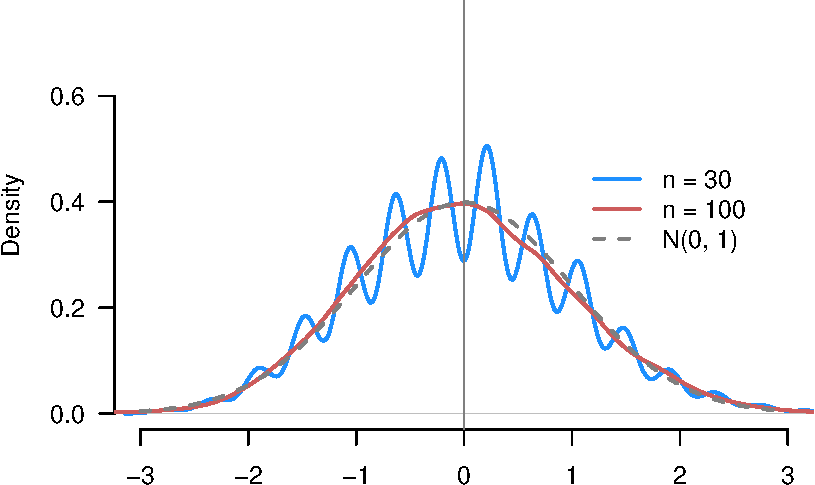
\includegraphics{03_asymptotics_files/figure-pdf/fig-clt-1.pdf}

}

\caption{\label{fig-clt}Sampling distributions of the normalized sample
mean at n=30 and n=100.}

\end{figure}

\end{example}

There are several properties of convergence in distribution that are
helpful to us.

\begin{theorem}[Properties of convergence in
distribution]\protect\hypertarget{thm-indist-properties}{}\label{thm-indist-properties}

Let \(X_n\) be a sequence of random variables \(X_1, X_2,\ldots\) that
converges in distribution to some rv \(X\) and let \(Y_n\) be a sequence
of random variables \(Y_1, Y_2,\ldots\) that converges in probability to
some number, \(c\). Then,

\begin{enumerate}
\def\labelenumi{\arabic{enumi}.}
\tightlist
\item
  \(g(X_n) \indist g(X)\) for all continuous functions \(g\).
\item
  \(X_nY_n\) converges in distribution to \(cX\)
\item
  \(X_n + Y_n\) converges in distribution to \(X + c\)
\item
  \(X_n / Y_n\) converges in distribution to \(X / c\) if \(c \neq 0\)
\end{enumerate}

\end{theorem}

We refer to the last three results as \textbf{Slutsky's theorem}. These
results are often crucial for determining an estimator's asymptotic
distribution.

A critical application of Slutsky's theorem is when we replace the
(unknown) population variance in the CLT with an estimate. Recall the
definition of the \textbf{sample variance} as \[
S_n^2 = \frac{1}{n-1} \sum_{i=1}^n (X_i - \Xbar_n)^2,
\] with the \textbf{sample standard deviation} defined as
\(S_{n} = \sqrt{S_{n}^2}\). It's easy to show that these are consistent
estimators for their respective population parameters \[ 
S_{n}^2 \inprob \sigma^2 = \V[X_i], \qquad S_{n} \inprob \sigma,
\] which, by Slutsky's theorem, implies that \[
\frac{\sqrt{n}\left(\Xbar_n - \mu\right)}{S_n} \indist \N(0, 1)
\] Comparing this result to the statement of CLT, we see that replacing
the population variance with a consistent estimate of the variance (or
standard deviation) does not affect the asymptotic distribution.

Like with the WLLN, the CLT holds for random vectors of sample means,
where their centered and scaled versions converge to a multivariate
normal distribution with a covariance matrix equal to the covariance
matrix of the underlying random vectors of data, \(\X_i\).

\begin{theorem}[]\protect\hypertarget{thm-multivariate-clt}{}\label{thm-multivariate-clt}

If \(\mb{X}_i \in \mathbb{R}^k\) are i.i.d. and
\(\E\Vert \mb{X}_i \Vert^2 < \infty\), then as \(n \to \infty\), \[
\sqrt{n}\left( \overline{\mb{X}}_n - \mb{\mu}\right) \indist \N(0, \mb{\Sigma}),
\] where \(\mb{\mu} = \E[\mb{X}_i]\) and
\(\mb{\Sigma} = \V[\mb{X}_i] = \E\left[(\mb{X}_i-\mb{\mu})(\mb{X}_i - \mb{\mu})'\right]\).

\end{theorem}

Notice that \(\mb{\mu}\) is the vector of population means for all the
random variables in \(\X_i\) and \(\mb{\Sigma}\) is the
variance-covariance matrix for that vector.

\begin{tcolorbox}[enhanced jigsaw, colbacktitle=quarto-callout-note-color!10!white, colframe=quarto-callout-note-color-frame, arc=.35mm, left=2mm, toptitle=1mm, rightrule=.15mm, title=\textcolor{quarto-callout-note-color}{\faInfo}\hspace{0.5em}{Note}, colback=white, leftrule=.75mm, toprule=.15mm, coltitle=black, opacityback=0, breakable, bottomtitle=1mm, titlerule=0mm, bottomrule=.15mm, opacitybacktitle=0.6]

As with the notation alert with the WLLN, we are using shorthand here,
\(\E\Vert \mb{X}_i \Vert^2 < \infty\), which implies that
\(\E[X_{ij}^2] < \infty\) for all \(j = 1,\ldots, k\), or equivalently,
that the variances of each variable in the sample means has finite
variance.

\end{tcolorbox}

\hypertarget{confidence-intervals}{%
\section{Confidence intervals}\label{confidence-intervals}}

We now turn to an essential application of the central limit theorem:
confidence intervals.

You have run your experiment and presented your readers with your single
best guess about the treatment effect with the difference in sample
means. You may have also presented the estimated standard error of this
estimate to give readers a sense of how variable the estimate is. But
none of these approaches answer a fairly compelling question: what range
of values of the treatment effect is \textbf{plausible} given the data
we observe?

A point estimate typically has 0 probability of being the exact true
value, but intuitively we hope that the true value is close to this
estimate. \textbf{Confidence intervals} make this kind of intuition more
formal by instead estimating ranges of values with a fixed percentage of
these ranges containing the actual parameter value.

We begin with the basic definition of a confidence interval.

\begin{definition}[]\protect\hypertarget{def-coverage}{}\label{def-coverage}

A \(1-\alpha\) \textbf{confidence interval} for a real-valued parameter
\(\theta\) is a pair of statistics \(L= L(X_1, \ldots, X_n)\) and
\(U = U(X_1, \ldots, X_n)\) such that \(L < U\) for all values of the
sample and such that \[ 
\P(L \leq \theta \leq U \mid \theta) \geq 1-\alpha, \quad \forall \theta \in \Theta.
\]

\end{definition}

We say that a \(1-\alpha\) confidence interval covers (contains,
captures, traps, etc.) the true value at least \(100(1-\alpha)\%\) of
the time, and we refer to \(1-\alpha\) as the \textbf{coverage
probability} or simply \textbf{coverage}. Typical confidence intervals
include 95\% percent (\(\alpha = 0.05\)) and 90\% (\(\alpha = 0.1\)).

So a confidence interval is a random interval with a particular
guarantee about how often it will contain the true value. It's important
to remember what is random and what is fixed in this setup. The interval
varies from sample to sample, but the true value of the parameter stays
fixed, and the coverage is how often we should expect the interval to
contain that true value. The ``repeating my sample over and over again''
analogy can break down very quickly, so it's sometimes helpful to
interpret it as giving guarantees across confidence intervals across
different experiments. In particular, suppose that a journal publishes
100 quantitative articles annually, each producing a single 95\%
confidence interval for their quantity of interest. Then, if the
confidence intervals are valid, we should expect 95 of those confidence
intervals to contain the true value.

\begin{tcolorbox}[enhanced jigsaw, colbacktitle=quarto-callout-warning-color!10!white, colframe=quarto-callout-warning-color-frame, arc=.35mm, left=2mm, toptitle=1mm, rightrule=.15mm, title=\textcolor{quarto-callout-warning-color}{\faExclamationTriangle}\hspace{0.5em}{Warning}, colback=white, leftrule=.75mm, toprule=.15mm, coltitle=black, opacityback=0, breakable, bottomtitle=1mm, titlerule=0mm, bottomrule=.15mm, opacitybacktitle=0.6]

Suppose you calculate a 95\% confidence interval, \([0.1, 0.4]\). It's
tempting to make a probability statement like
\(\P(0.1 \leq \theta \leq 0.4 \mid \theta) = 0.95\) or that there's a
95\% chance that the parameter is in \([0.1, 0.4]\). But looking at the
probability statement, everything on the left-hand side of the
conditioning bar is fixed, so the probability either has to be 0
(\(\theta\) is outside the interval) or 1 (\(\theta\) is in the
interval). The coverage probability of a confidence interval refers to
its status as a pair of random variables, \((L, U)\), not any particular
realization of those variables like \((0.1, 0.4)\). As an analogy,
consider if calculated the sample mean as \(0.25\) and then try to say
that \(0.25\) is unbiased for the population mean. This statement
doesn't make sense because unbiasedness refers to how the sample mean
varies from sample to sample.

\end{tcolorbox}

In most cases, we will not be able to derive exact confidence intervals
but rather confidence intervals that are \textbf{asymptotically valid},
which means that if we write the interval as a function of the sample
size, \((L_n, U_n)\), they would have \textbf{asymptotic coverage} \[
\lim_{n\to\infty} \P(L_n \leq \theta \leq U_n) \geq 1-\alpha \quad\forall\theta\in\Theta.
\]

Asymptotic coverage is the property we can show for most confidence
intervals since we usually rely on large sample approximations based on
the central limit theorem.

\hypertarget{deriving-confidence-intervals}{%
\subsection{Deriving confidence
intervals}\label{deriving-confidence-intervals}}

If you have taken any statistics before, you probably have seen the
standard formula for the 95\% confidence interval of the sample mean,
\[ 
\left[\Xbar_n - 1.96\frac{s}{\sqrt{n}},\; \Xbar_n + 1.96\frac{s}{\sqrt{n}}\right],
\] where you can recall that \(s\) is the sample standard deviation and
\(s/\sqrt{n}\) is the estimate of the standard error of the sample mean.
If this is a 95\% confidence interval, then the probability that it
contains the population mean \(\mu\) should be 0.95, but how can we
derive this? We can justify this logic using the central limit theorem,
and the argument will hold for any asymptotically normal estimator.

Let's say that we have an estimator, \(\widehat{\theta}_n\) for the
parameter \(\theta\) with estimated standard error
\(\widehat{\se}[\widehat{\theta}_n]\). If the estimator is
asymptotically normal, then in large samples, we know that \[ 
\frac{\widehat{\theta}_n - \theta}{\widehat{\se}[\widehat{\theta}_n]} \sim \N(0, 1).
\] We can then use our knowledge of the standard normal and the
empirical rule to find \[ 
\P\left( -1.96 \leq \frac{\widehat{\theta}_n - \theta}{\widehat{\se}[\widehat{\theta}_n]} \leq 1.96\right) = 0.95
\] and by multiplying each part of the inequality by
\(\widehat{\se}[\widehat{\theta}_n]\), we get \[ 
\P\left( -1.96\,\widehat{\se}[\widehat{\theta}_n] \leq \widehat{\theta}_n - \theta \leq 1.96\,\widehat{\se}[\widehat{\theta}_n]\right) = 0.95,
\] We then subtract all parts by the estimator to get \[ 
\P\left(-\widehat{\theta}_n - 1.96\,\widehat{\se}[\widehat{\theta}_n] \leq - \theta \leq -\widehat{\theta}_n + 1.96\,\widehat{\se}[\widehat{\theta}_n]\right) = 0.95,
\] and finally we multiply all parts by \(-1\) (and flipping the
inequalities) to arrive at \[ 
\P\left(\widehat{\theta}_n - 1.96\,\widehat{\se}[\widehat{\theta}_n] \leq \theta \leq \widehat{\theta}_n + 1.96\,\widehat{\se}[\widehat{\theta}_n]\right) = 0.95.
\] To connect back to the definition of the confidence interval, we have
now shown that the random interval \([L, U]\) where \[ 
\begin{aligned}
  L = L(X_1, \ldots, X_n) &= \widehat{\theta}_n - 1.96\,\widehat{\se}[\widehat{\theta}_n] \\
  U = U(X_1, \ldots, X_n) &= \widehat{\theta}_n + 1.96\,\widehat{\se}[\widehat{\theta}_n],
\end{aligned}
\] is an asymptotically valid estimator.\footnote{The analysis here
  largely comes from Senn (2012).} Replacing \(\Xbar_n\) for
\(\widehat{\theta}_n\) and \(s/\sqrt{n}\) for
\(\widehat{\se}[\widehat{\theta}_n]\) establishes how the standard 95\%
confidence interval for the sample mean above is asymptotically valid.

\begin{figure}

{\centering 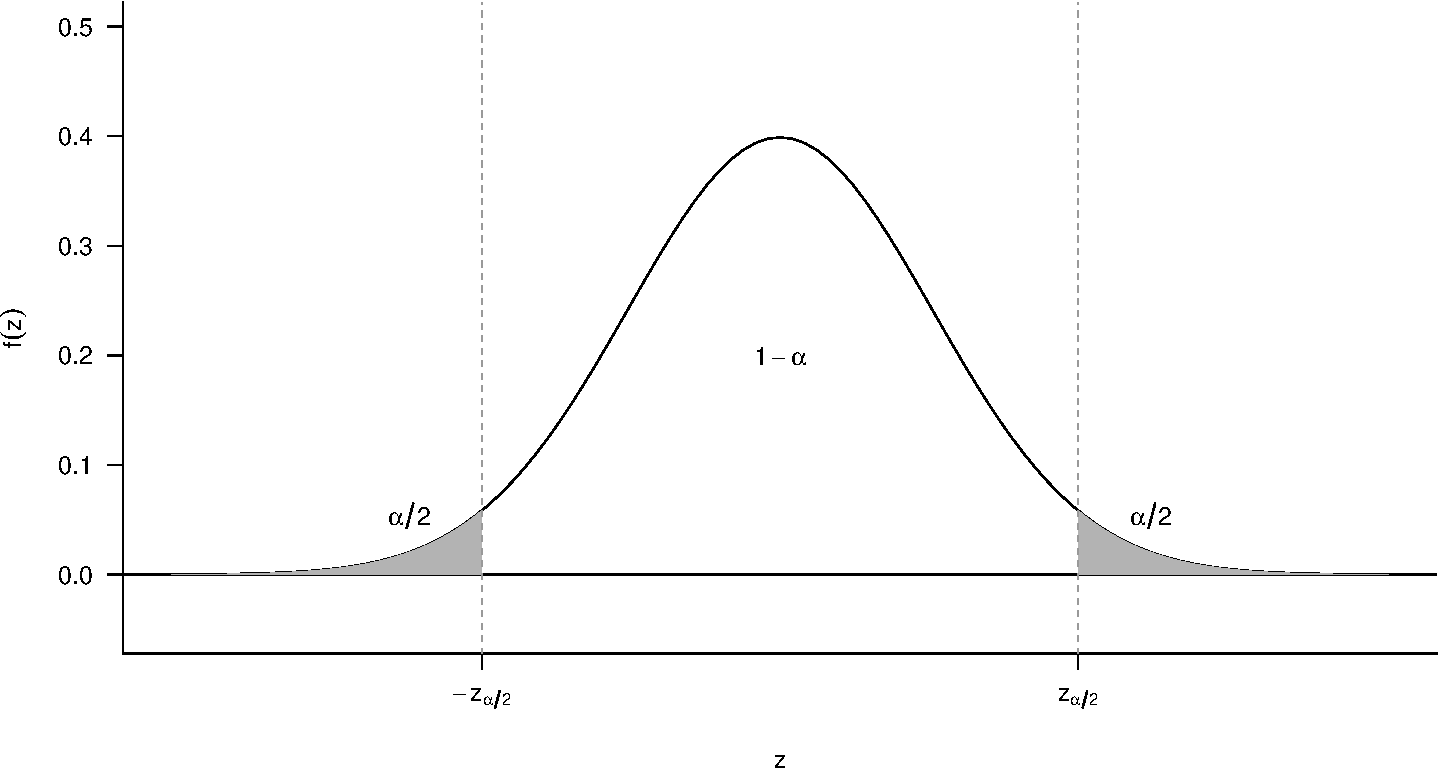
\includegraphics{03_asymptotics_files/figure-pdf/fig-std-normal-1.pdf}

}

\caption{\label{fig-std-normal}Critical values for the standard normal.}

\end{figure}

How can we generalize this to \(1-\alpha\) confidence intervals? For a
standard normal rv, \(Z\), we know that \[ 
\P(-z_{\alpha/2} \leq Z \leq z_{\alpha/2}) = 1-\alpha
\] which implies that we can obtain a \(1-\alpha\) asymptotic confidence
intervals by using the interval \([L, U]\), where \[ 
L = \widehat{\theta}_{n} - z_{\alpha/2} \widehat{\se}[\widehat{\theta}_{n}], \quad U = \widehat{\theta}_{n} + z_{\alpha/2} \widehat{\se}[\widehat{\theta}_{n}]. 
\] This is sometimes shortened to
\(\widehat{\theta}_n \pm z_{\alpha/2} \widehat{\se}[\widehat{\theta}_{n}]\).
Remember that we can obtain the values of \(z_{\alpha/2}\) easily from
R:

\begin{Shaded}
\begin{Highlighting}[]
\DocumentationTok{\#\# alpha = 0.1 for 90\% CI}
\FunctionTok{qnorm}\NormalTok{(}\FloatTok{0.1} \SpecialCharTok{/} \DecValTok{2}\NormalTok{, }\AttributeTok{lower.tail =} \ConstantTok{FALSE}\NormalTok{)}
\end{Highlighting}
\end{Shaded}

\begin{verbatim}
[1] 1.644854
\end{verbatim}

As a concrete example, then, we could derive a 90\% asymptotic
confidence interval for the sample mean as \[ 
\left[\Xbar_{n} - 1.64 \frac{\widehat{\sigma}}{\sqrt{n}}, \Xbar_{n} + 1.64 \frac{\widehat{\sigma}}{\sqrt{n}}\right]
\]

\hypertarget{interpreting-confidence-intervals}{%
\subsection{Interpreting confidence
intervals}\label{interpreting-confidence-intervals}}

Remember that the interpretation of confidence is how the random
interval performs over repeated samples. A valid 95\% confidence
interval is a random interval containing the true value in 95\% of
samples. Simulating repeated samples helps clarify this.

\begin{example}[]\protect\hypertarget{exm-cis}{}\label{exm-cis}

Suppose we are taking samples of size \(n=500\) of random variables
where \(X_i \sim \N(1, 10)\), and we want to estimate the population
mean \(\E[X] = 1\). To do so, we repeat the following steps:

\begin{enumerate}
\def\labelenumi{\arabic{enumi}.}
\tightlist
\item
  Draw a sample of \(n=500\) from \(\N(1, 10)\).
\item
  Calculate the 95\% confidence interval sample mean
  \(\Xbar_n \pm 1.96\widehat{\sigma}/\sqrt{n}\).
\item
  Plot the intervals along the x-axis and color them blue if they
  contain the truth (1) and red if not.
\end{enumerate}

Figure~\ref{fig-ci-sim} shows 100 iterations of these steps. We see
that, as expected, most calculated CIs contain the true value. Five
random samples produce intervals that fail to include 1, an exact
coverage rate of 95\%. Of course, this is just one simulation, and a
different set of 100 random samples might have produced a slightly
different coverage rate. The guarantee of the 95\% confidence intervals
is that if we were to continue to take these repeated samples, the
long-run frequency of intervals covering the truth would approach 0.95.

\begin{figure}

{\centering 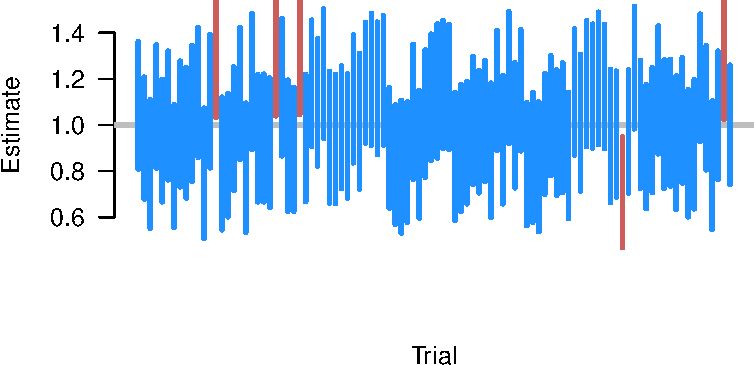
\includegraphics{03_asymptotics_files/figure-pdf/fig-ci-sim-1.pdf}

}

\caption{\label{fig-ci-sim}95\% confidence intervals from 100 random
samples. Intervals are blue if they contain the truth and red if they do
not.}

\end{figure}

\end{example}

\hypertarget{sec-delta-method}{%
\section{Delta method}\label{sec-delta-method}}

Suppose that we know that an estimator follows the CLT, and so we have
\[
\sqrt{n}\left(\widehat{\theta}_n - \theta \right) \indist \N(0, V),
\] but we actually want to estimate \(h(\theta)\) so we use the plug-in
estimator, \(h(\widehat{\theta}_n)\). It seems like we should be able to
apply part 1 of Theorem~\ref{thm-indist-properties}. Still, the CLT
established the large-sample distribution of the centered and scaled
random sequence, \(\sqrt{n}(\widehat{\theta}_n - \theta)\), not to the
original estimator itself like we would need to investigate the
asymptotic distribution of \(h(\widehat{\theta}_n)\). We can use a
little bit of calculus to get an approximation of the distribution we
need.

\begin{theorem}[]\protect\hypertarget{thm-delta-method}{}\label{thm-delta-method}

If \(\sqrt{n}\left(\widehat{\theta}_n - \theta\right) \indist \N(0, V)\)
and \(h(u)\) is continuously differentiable in a neighborhood around
\(\theta\), then as \(n\to\infty\), \[
\sqrt{n}\left(h(\widehat{\theta}_n) - h(\theta) \right) \indist \N(0, (h'(\theta))^2 V).
\]

\end{theorem}

Understanding what's happening here is useful since it might help give
intuition as to when this might go wrong. Why do we focus on
continuously differentiable functions, \(h()\)? These functions can be
well-approximated with a line in a neighborhood around a given point
like \(\theta\). In Figure~\ref{fig-delta}, we show this where the
tangent line at \(\theta_0\), which has slope \(h'(\theta_0)\), is very
similar to \(h(\theta)\) for values close to \(\theta_0\). Because of
this, we can approximate the difference between
\(h(\widehat{\theta}_n)\) and \(h(\theta_0)\) with the what this tangent
line would give us: \[
\underbrace{\left(h(\widehat{\theta_n}) - h(\theta_0)\right)}_{\text{change in } y} \approx \underbrace{h'(\theta_0)}_{\text{slope}} \underbrace{\left(\widehat{\theta}_n - \theta_0\right)}_{\text{change in } x},
\] and then multiplying both sides by the \(\sqrt{n}\) gives \[
\sqrt{n}\left(h(\widehat{\theta_n}) - h(\theta_0)\right) \approx h'(\theta_0)\sqrt{n}\left(\widehat{\theta}_n - \theta_0\right). 
\] The right-hand side of this approximation converges to
\(h'(\theta_0)Z\), where \(Z\) is a random variable with \(\N(0, V)\).
The variance of this quantity will be \[
\V[h'(\theta_0)Z] = (h'(\theta_0))^2\V[Z] = (h'(\theta_0))^2V,
\] by the properties of variances.

\begin{figure}

{\centering 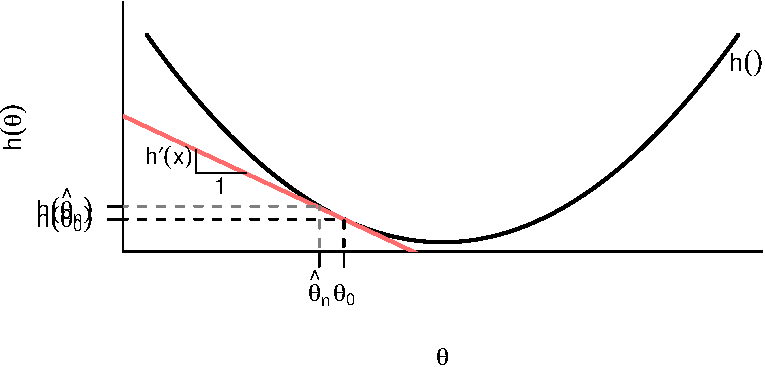
\includegraphics{03_asymptotics_files/figure-pdf/fig-delta-1.pdf}

}

\caption{\label{fig-delta}Linear approximation to nonlinear functions.}

\end{figure}

\begin{example}[]\protect\hypertarget{exm-log}{}\label{exm-log}

Let's return to the iid sample \(X_1, \ldots, X_n\) with mean
\(\mu = \E[X_i]\) and variance \(\sigma^2 = \V[X_i]\). From the CLT, we
know that \(\sqrt{n}(\Xbar_n - \mu) \indist \N(0, \sigma^2)\). Suppose
that we want to estimate \(\log(\mu)\), so we use the plug-in estimator
\(\log(\Xbar_n)\) (assuming that \(X_i > 0\) for all \(i\) so that we
can take the log). What is the asymptotic distribution of this
estimator? This is a situation where \(\widehat{\theta}_n = \Xbar_n\)
and \(h(\mu) = \log(\mu)\). From basic calculus, we know that \[
h'(\mu) = \frac{\partial \log(\mu)}{\partial \mu} = \frac{1}{\mu},
\] so applying the delta method, we can determine that \[
\sqrt{n}\left(\log(\Xbar_n) - \log(\mu)\right) \indist \N\left(0,\frac{\sigma^2}{\mu^2} \right).
\]

\end{example}

\begin{example}[]\protect\hypertarget{exm-exp}{}\label{exm-exp}

What about estimating the \(\exp(\mu)\) with \(\exp(\Xbar_n)\)? Recall
that \[
h'(\mu) = \frac{\partial \exp(\mu)}{\partial \mu} = \exp(\mu)
\] so applying the delta method, we have \[
\sqrt{n}\left(\exp(\Xbar_n) - \exp(\mu)\right) \indist \N(0, \exp(2\mu)\sigma^2),
\] since \(\exp(\mu)^2 = \exp(2\mu)\).

\end{example}

Like all of the results in this chapter, there is a multivariate version
of the delta method that is incredibly useful in practical applications.
We often will combine two different estimators (or two different
estimated parameters) to estimate another quantity. We now let
\(\mb{h}(\mb{\theta}) = (h_1(\mb{\theta}), \ldots, h_m(\mb{\theta}))\)
map from \(\mathbb{R}^k \to \mathbb{R}^m\) and be continuously
differentiable (we make the function bold since it returns an
\(m\)-dimensional vector). It will help us to use more compact matrix
notation if we introduce a \(m \times k\) Jacobian matrix of all partial
derivatives \[
\mb{H}(\mb{\theta}) = \mb{\nabla}_{\mb{\theta}}\mb{h}(\mb{\theta}) = \begin{pmatrix}
  \frac{\partial h_1(\mb{\theta})}{\partial \theta_1} & \frac{\partial h_1(\mb{\theta})}{\partial \theta_2} & \cdots & \frac{\partial h_1(\mb{\theta})}{\partial \theta_k} \\
  \frac{\partial h_2(\mb{\theta})}{\partial \theta_1} & \frac{\partial h_2(\mb{\theta})}{\partial \theta_2} & \cdots & \frac{\partial h_2(\mb{\theta})}{\partial \theta_k} \\
  \vdots & \vdots & \ddots & \vdots \\
  \frac{\partial h_m(\mb{\theta})}{\partial \theta_1} & \frac{\partial h_m(\mb{\theta})}{\partial \theta_2} & \cdots & \frac{\partial h_m(\mb{\theta})}{\partial \theta_k} 
\end{pmatrix},
\] which we can use to generate the equivalent multivariate linear
approximation \[
\left(\mb{h}(\widehat{\mb{\theta}}_n) - \mb{h}(\mb{\theta}_0)\right) \approx \mb{H}(\mb{\theta}_0)'\left(\widehat{\mb{\theta}}_n - \mb{\theta}_0\right).
\] We can use this fact to derive the multivariate delta method.

\begin{theorem}[]\protect\hypertarget{thm-multivariate-delta}{}\label{thm-multivariate-delta}

Suppose that
\(\sqrt{n}\left(\widehat{\mb{\theta}}_n - \mb{\theta}_0 \right) \indist \N(0, \mb{\Sigma})\),
then for any function \(\mb{h}\) that is continuously differentiable in
a neighborhood of \(\mb{\theta}_0\), we have \[
\sqrt{n}\left(\mb{h}(\widehat{\mb{\theta}}_n) - \mb{h}(\mb{\theta}_0) \right) \indist \N(0, \mb{H}\mb{\Sigma}\mb{H}'), 
\] where \(\mb{H} = \mb{H}(\mb{\theta}_0)\).

\end{theorem}

This result follows from the approximation above plus rules about
variances of random vectors. Remember that for any compatible matrix of
constants, \(\mb{A}\), we have
\(\V[\mb{A}'\mb{Z}] = \mb{A}\V[\mb{Z}]\mb{A}'\). You can see that the
matrix of constants appears twice here, like the matrix version of the
``squaring the constant'' rule for variance.

The delta method is handy for generating closed-form approximations for
asymptotic standard errors, but the math is often quite complex for even
simple estimators. It is usually more straightforward for applied
researchers to use computational tools like the bootstrap to approximate
the standard errors we need. The bootstrap has the trade-off of taking
more computational time to implement than the delta method. Still, it is
more easily adaptable across different estimators and domains with
little human thinking time.

\hypertarget{hypothesis-tests}{%
\chapter{Hypothesis tests}\label{hypothesis-tests}}

Up to now, we have discussed the properties of estimators that allow us
to characterize their distributions in finite and large samples. These
properties might let us say that, for example, our estimated difference
in means is equal to a true average treatment effect on average across
repeated samples or that it will converge to the true value in large
samples. These properties, however, are properties of repeated samples.
As researchers, we will only have access to a single sample.
\textbf{Statistical inference} is the process of using our single sample
to learn about population parameters. Several ways to conduct inference
are connected, but one of the most ubiquitous in the sciences is the
hypothesis test, which is a kind of statistical thought experiment.

\hypertarget{the-lady-tasting-tea}{%
\section{The lady tasting tea}\label{the-lady-tasting-tea}}

The lady tasting tea exemplifies the core ideas behind hypothesis
testing due to R.A. Fisher.\footnote{The analysis here largely comes
  from Senn (2012).} Fisher had prepared tea for his colleague, the
algologist Muriel Bristol. Knowing that she preferred milk in her tea,
he poured milk into a tea cup and then poured the hot tea into the milk.
Bristol rejected the cup, stating that she preferred pouring the tea
first, then milk. Fisher was skeptical at the idea anyone could tell the
difference between a cup poured milk-first or tea-first. So he and
another colleague, William Roach, devised a test to see if Bristol could
distinguish the two preparation methods.

Fisher and Roach prepared 8 cups of tea, four milk-first and four
tea-first. They then presented the cups to Bristol in a random order
(though she knew there were 4 of each type), and she proceeded to
identify all of the cups correctly. At first glance, this seems like
good evidence that she can tell the difference between the two types,
but a skeptic like Fisher raised the question: ``could she have just
been randomly guessing and got lucky?'' This led Fisher to a
\textbf{statistical thought experiment}: what would the probability of
guessing the correct cups be \emph{if} she were guessing randomly?

To calculate the probability of Bristol's achievement, we can note that
``randomly guessing'' here would mean that she was selecting a group of
4 cups to be labeled milk-first from the 8 cups available. Using basic
combinatorics, we can calculate there are 70 ways to choose 4 cups among
8, but only 1 of those arrangements would be correct. Thus, if randomly
guessing means choosing among those 70 options with equal chance, then
the probability of guessing the right set of cups is 1/70 or
\(\approx 0.014\). The low probability implies that the hypothesis of
random guessing may be implausible.

The story of the lady tasting tea encapsulates many of the core elements
of hypothesis testing. Hypothesis testing is about taking our observed
estimate (Bristol guessing all the cups correctly) and seeing how likely
that observed estimate would be under some assumption or hypothesis
about the data-generating process (Bristol was randomly guessing). When
the observed estimate is unlikely under the maintained hypothesis, we
might view this as evidence against that hypothesis. Thus, hypothesis
tests help us assess evidence for particular guesses about the DGP.

\begin{tcolorbox}[enhanced jigsaw, colbacktitle=quarto-callout-note-color!10!white, colframe=quarto-callout-note-color-frame, arc=.35mm, left=2mm, toptitle=1mm, rightrule=.15mm, title=\textcolor{quarto-callout-note-color}{\faInfo}\hspace{0.5em}{Notation alert}, colback=white, leftrule=.75mm, toprule=.15mm, coltitle=black, opacityback=0, breakable, bottomtitle=1mm, titlerule=0mm, bottomrule=.15mm, opacitybacktitle=0.6]

For the rest of this chapter, we'll introduce the concepts following the
notation in the past chapters. We'll usually assume that we have a
random (iid) sample of random variables \(X_1, \ldots, X_n\) from a
distribution, \(F\). We'll focus on estimating some parameter,
\(\theta\), of this distribution (like the mean, median, variance,
etc.). We'll refer to \(\Theta\) as the set of possible values of
\(\theta\) or the \textbf{parameter space}.

\end{tcolorbox}

\hypertarget{hypotheses}{%
\section{Hypotheses}\label{hypotheses}}

In the context of hypothesis testing, hypotheses are just statements
about the population distribution. In particular, we will make
statements that \(\theta = \theta_0\) where \(\theta_0 \in \Theta\) is
the hypothesized value of \(\theta\). Hypotheses are ubiquitous in
empirical work, but here are some examples to give you a flavor:

\begin{itemize}
\tightlist
\item
  The population proportion of US citizens that identify as Democrats is
  0.33.
\item
  The population difference in average voter turnout between households
  who received get-out-the-vote mailers vs.~those who did not is 0.
\item
  The difference in the average incidence of human rights abuse in
  countries that signed a human rights treaty vs.~those countries that
  did not sign is 0.
\end{itemize}

Each of these is a statement about the true DGP. The latter two are very
common: when \(\theta\) represents the difference in means between two
groups, then \(\theta = 0\) is the hypothesis of no actual difference in
population means or no treatment effect (if the causal effect is
identified).

The goal of hypothesis testing is to adjudicate between two
complementary hypotheses.

\begin{definition}[]\protect\hypertarget{def-null}{}\label{def-null}

The two hypotheses in a hypothesis test are called the \textbf{null
hypothesis} and the \textbf{alternative hypothesis}, denoted as \(H_0\)
and \(H_1\), respectively.

\end{definition}

These hypotheses are complementary, so if the null hypothesis
\(H_0: \theta \in \Theta_0\), then the alternative hypothesis is
\(H_1: \theta \in \Theta_0^c\). The ``null'' in null hypothesis might
seem odd until you realize that most null hypotheses are that there is
no effect of some treatment or no difference in means. For example,
suppose \(\theta\) is the difference in mean support for expanding legal
immigration between a treatment group that received a pro-immigrant
message and some facts about immigration and a control group that just
received the factual information. Then, the typical null hypothesis
would be no difference in means or \(H_0: \theta = 0\), and the
alternative would be \(H_1: \theta \neq 0\).

There are two types of tests that differ in the form of their null and
alternative hypotheses. A \textbf{two-sided test} is of the form \[
H_0: \theta = \theta_0 \quad\text{versus}\quad H_1: \theta \neq \theta_0,
\] where the ``two-sided'' part refers to how the alternative contains
values of \(\theta\) above and below the null value \(\theta_0\). A
\textbf{one-sided test} has the form \[
H_0: \theta \leq \theta_0 \quad\text{versus}\quad H_1: \theta > \theta_0,
\] or \[
H_0: \theta \geq \theta_0 \quad\text{versus}\quad H_1: \theta < \theta_0.
\] Two-sided tests are much more common in the social sciences, where we
want to know if there is any evidence, positive or negative, against the
presumption of no treatment effect or no relationship between two
variables. One-sided tests are for situations where we only want
evidence in one direction, which is rarely relevant to social science
research. One-sided tests also have the downside of being misused to
inflate the strength of evidence against the null and should be avoided.
Unfortunately, the math of two-sided tests is also more complicated.

\hypertarget{the-procedure-of-hypothesis-testing}{%
\section{The procedure of hypothesis
testing}\label{the-procedure-of-hypothesis-testing}}

At the most basic level, a \textbf{hypothesis test} is a rule that
specifies values of the sample data for which we will decide to
\textbf{reject} the null hypothesis. Let \(\mathcal{X}_n\) be the range
of the sample---that is, all possible vectors \((x_1, \ldots, x_n)\)
that have a positive probability of occurring. Then, a hypothesis test
describes a region of this space, \(R \subset \mathcal{X}_n\), called
the \textbf{rejection region} where when \((X_1, \ldots, X_n) \in R\) we
will \textbf{reject} \(H_0\) and when the data is outside this region,
\((X_1, \ldots, X_n) \notin R\) we \textbf{retain}, \textbf{accept}, or
\textbf{fail to reject} the null hypothesis.\footnote{Different people
  and different textbooks describe what to do when we do not reject the
  null hypothesis in different ways. The terminology is not so important
  so long as you understand that rejecting the null does not mean the
  null is logically false, and ``accepting'' the null does not mean the
  null is logically true.}

How do we decide what the rejection region should be? Even though we
define the rejection region in terms of the \textbf{sample space},
\(\mathcal{X}_n\), it's unwieldy to work with the entire vector of data.
Instead, we often formulate the rejection region in terms of a
\textbf{test statistic}, \(T = T(X_1, \ldots, X_n)\), where the
rejection region becomes \[
R = \left\{(x_1, \ldots, x_n) : T(x_1, \ldots, x_n) > c\right\},
\] where \(c\) is called the \textbf{critical value}. This expression
says that the rejection region is the part of the sample space that
makes the test statistic sufficiently large. We reject null hypotheses
when the observed data is incompatible with those hypotheses, where the
test statistic should be a measure of this incompatibility. Note that
the test statistic is a random variable and has a distribution---we will
exploit this to understand the different properties of a hypothesis
test.

\begin{example}[]\protect\hypertarget{exm-biden}{}\label{exm-biden}

Suppose that \((X_1, \ldots, X_n)\) represents a sample of US citizens
where \(X_i = 1\) indicates support for the current US president and
\(X_i = 0\) means no support. We might be interested in the test of the
null hypothesis that the president does not have the support of a
majority of American citizens. Let \(\mu = \E[X_i] = \P(X_i = 1)\).
Then, a one-sided test would compare the two hypotheses: \[ 
H_0: \mu \leq 0.5 \quad\text{versus}\quad H_1: \mu > 0.5.
\] In this case, we might use the sample mean as the test statistic, so
that \(T(X_1, \ldots, X_n) = \Xbar_n\) and we have to find some
threshold above 0.5 such that we would reject the null, \[ 
R = \left\{(x_1, \ldots, x_n): \Xbar_n > c\right\}.
\] In words, how much support should we see for the current president
before we reject the notion that they lack majority support? Below we
will select the critical value, \(c\), to have beneficial statistical
properties.

\end{example}

The structure of a reject region will depend on whether a test is one-
or two-sided. One-sided tests will take the form \(T > c\), whereas
two-sided tests will take the form \(|T| > c\) since we want to count
deviations from either side of the null hypothesis as evidence against
that null.

\hypertarget{testing-errors}{%
\section{Testing errors}\label{testing-errors}}

Hypothesis tests end with a decision to reject the null hypothesis or
not, but this might be an incorrect decision. In particular, there are
two ways to make errors and two ways to be correct in this setting, as
shown in Table~\ref{tbl-errors}. The labels are confusing, but it's
helpful to remember that \textbf{type I errors} (said ``type one'') are
labeled so because they are the worse of the two types of errors. These
errors occur when we reject a null (say there is a true treatment effect
or relationship) when the null is true (there is no true treatment
effect or relationship). Type I errors are what we see in the
replication crisis: lots of ``significant'' effects that turn out later
to be null. \textbf{Type II errors} (said ``type two'') are considered
less problematic: there is a true relationship, but we cannot detect it
with our test (we cannot reject the null).

\hypertarget{tbl-errors}{}
\begin{longtable}[]{@{}lll@{}}
\caption{\label{tbl-errors}Typology of testing errors}\tabularnewline
\toprule\noalign{}
& \(H_0\) True & \(H_0\) False \\
\midrule\noalign{}
\endfirsthead
\toprule\noalign{}
& \(H_0\) True & \(H_0\) False \\
\midrule\noalign{}
\endhead
\bottomrule\noalign{}
\endlastfoot
Retain \(H_0\) & Awesome & Type II error \\
Reject \(H_0\) & Type I error & Great \\
\end{longtable}

Ideally, we would minimize the chances of making either a type I or type
II error. Unfortunately, because the test statistic is a random
variable, we cannot remove the probability of an error altogether.
Instead, we will derive tests with some guaranteed performance to
minimize the probability of type I error. To derive this, we can define
the \textbf{power function} of a test, \[ 
\pi(\theta) = \P\left( \text{Reject } H_0 \mid \theta \right) = \P\left( T \in R \mid \theta \right),
\] which is the probability of rejection as a function of the parameter
of interest, \(\theta\). The power function tells us, for example, how
likely we are to reject the null of no treatment effect as we vary the
actual size of the treatment effect.

We can define the probability of type I error from the power function.

\begin{definition}[]\protect\hypertarget{def-size}{}\label{def-size}

The \textbf{size} of a hypothesis test with the null hypothesis
\(H_0: \theta = \theta_0\) is \[ 
\pi(\theta_0) = \P\left( \text{Reject } H_0 \mid \theta_0 \right).
\]

\end{definition}

You can think of the size of a test as the rate of false positives (or
false discoveries) produced by the test. Figure~\ref{fig-size-power}
shows an example of rejection regions, size, and power for a one-sided
test. In the left panel, we have the distribution of the test statistic
under the null, with \(H_0: \theta = \theta_0\), and the rejection
region is defined by values \(T > c\). The shaded grey region is the
probability of rejection under this null hypothesis or the size of the
test. Sometimes, we will get extreme samples by random chance, even
under the null, leading to false discoveries.\footnote{Eagle-eyed
  readers will notice that the null tested here is a point, while we
  previously defined the null in a one-sided test as a region
  \(H_0: \theta \leq \theta_0\). Technically, the size of the test will
  vary based on which of these nulls we pick. In this example, notice
  that any null to the left of \(\theta_0\) will result in a lower size.
  And so, the null at the boundary, \(\theta_0\), will maximize the size
  of the test, making it the most ``conservative'' null to investigate.
  Technically, we should define the size of a test as
  \(\alpha = \sup_{\theta \in \Theta_0} \pi(\theta)\).}

In the right panel, we overlay the distribution of the test statistic
under one particular alternative, \(\theta = \theta_1 > \theta_0\). The
red-shaded region is the probability of rejecting the null when this
alternative is true for the power---it's the probability of correctly
rejecting the null when it is false. Intuitively, we can see that
alternatives that produce test statistics closer to the rejection region
will have higher power. This makes sense: detecting big deviations from
the null should be easier than detecting minor ones.

\begin{figure}

{\centering 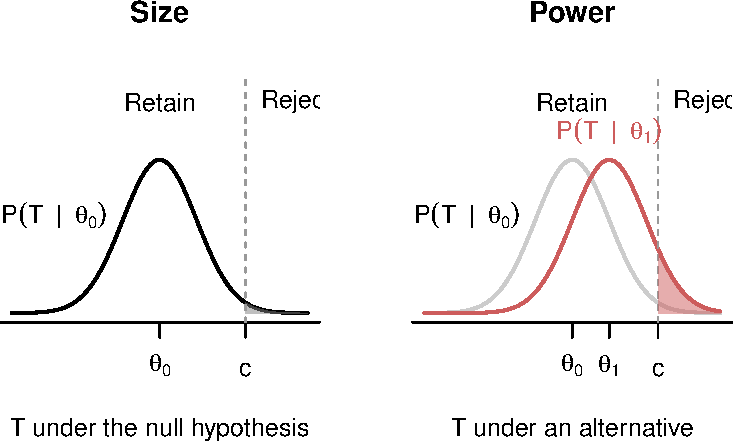
\includegraphics{04_hypothesis_tests_files/figure-pdf/fig-size-power-1.pdf}

}

\caption{\label{fig-size-power}Size of a test and power against an
alternative.}

\end{figure}

Figure~\ref{fig-size-power} also hints at a tradeoff between size and
power. Notice that we could make the size smaller (lower the false
positive rate) by increasing the critical value to \(c' > c\). This
would make the probability of being in the rejection region smaller,
\(\P(T > c' \mid \theta_0) < \P(T > c \mid \theta_0)\), leading to a
lower-sized test. Unfortunately, it would also reduce power in the right
panel since the probability of being in the rejection region will be
lower under any alternative,
\(\P(T > c' \mid \theta_1) < \P(T > c \mid \theta_1)\). This means we
usually cannot simultaneously reduce both types of errors.

\hypertarget{determining-the-rejection-region}{%
\section{Determining the rejection
region}\label{determining-the-rejection-region}}

If we cannot simultaneously optimize a test's size and power, how should
we determine where the rejection region is? That is, how should we
decide what empirical evidence will be strong enough for us to reject
the null? The standard approach to this problem in hypothesis testing is
to control the size of a test (that is, control the rate of false
positives) and try to maximize the power of the test subject to that
constraint. So we say, ``I'm willing to accept at most x\%'' of findings
will be false positives and do whatever we can to maximize power subject
to that constraint.

\begin{definition}[]\protect\hypertarget{def-level}{}\label{def-level}

A test has \textbf{significance level} \(\alpha\) if its size is less
than or equal to \(\alpha\), or \(\pi(\theta_0) \leq \alpha\).

\end{definition}

A test with a significance level of \(\alpha = 0.05\) will have a false
positive/type I error rate no larger than 0.05. This level is widespread
in the social sciences, though you also will see \(\alpha = 0.01\) or
\(\alpha = 0.1\). Frequentists justify this by saying this means that
with \(\alpha = 0.05\), there will only be at most 5\% of studies that
will produce false discoveries.

Our task is to construct the rejection region so that the \textbf{null
distribution} of the test statistic
\(G_0(t) = \P(T \leq t \mid \theta_0)\) has less than \(\alpha\)
probability in that region. One-sided tests like in
Figure~\ref{fig-size-power} are the easiest to show, even though we
warned you not to use them. We want to choose \(c\) that puts no more
than \(\alpha\) probability in the tail, or \[ 
\P(T > c \mid \theta_0) = 1 - G_0(c) \leq \alpha.
\] Remember that the smaller the value of \(c\) we can use will maximize
power, which implies that the critical value for the maximum power while
maintaining the significance level is when \(1 - G_0(c) = \alpha\). We
can use the \textbf{quantile function} of the null distribution to find
the exact value of \(c\) we need, \[
c = G^{-1}_0(1 - \alpha),
\] which is just fancy math to say, ``the value at which \(1-\alpha\) of
the null distribution is below.''

The determination of the rejection region follows the same principles
for two-sided tests, but it is slightly more complicated because we
reject when the magnitude of the test statistic is large, \(|T| > c\).
Figure~\ref{fig-two-sided} shows that basic setup. Notice that because
there are two (disjoint) regions, we can write the size (false positive
rate) as \[ 
\pi(\theta_0) = G_0(-c) + 1 - G_0(c).
\] In most cases that we will see, the null distribution for such a test
will be symmetric around 0 (usually asymptotically standard normal,
actually), which means that \(G_0(-c) = 1 - G_0(c)\), which implies that
the size is \[ 
\pi(\theta_0) = 2(1 - G_0(c)).
\] Solving for the critical value that would make this \(\alpha\) gives
\[ 
c = G^{-1}_0(1 - \alpha/2).
\] Again, this formula can seem dense, but remember what you are doing:
finding the value that puts \(\alpha/2\) of the probability of the null
distribution in each tail.

\begin{figure}

{\centering 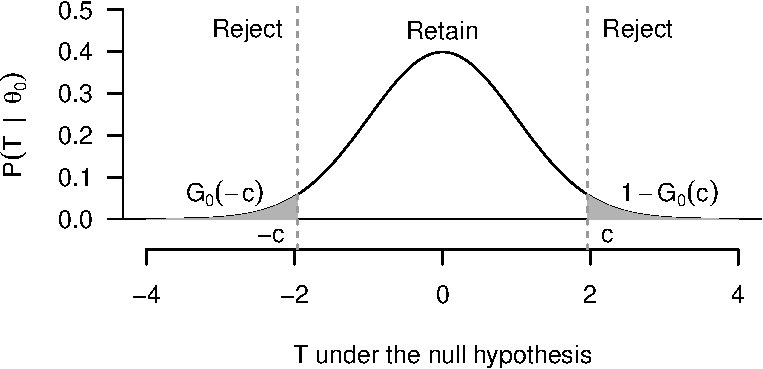
\includegraphics{04_hypothesis_tests_files/figure-pdf/fig-two-sided-1.pdf}

}

\caption{\label{fig-two-sided}Rejection regions for a two-sided test.}

\end{figure}

\hypertarget{hypothesis-tests-of-the-sample-mean}{%
\section{Hypothesis tests of the sample
mean}\label{hypothesis-tests-of-the-sample-mean}}

Let's go through an extended example about hypothesis testing of a
sample mean, sometimes called a \textbf{one-sample test}. Let's say
\(X_i\) are feeling thermometer scores about ``liberals'' as a group on
a scale of 0 to 100, with values closer to 0 indicating cooler feelings
about liberals and values closer to 100 indicating warmer feelings about
liberals. We want to know if the population average differs from a
neutral value of 50. We can write this two-sided test as \[
H_0: \mu = 50 \quad\text{versus}\quad H_1: \mu \neq 50,
\] where \(\mu = \E[X_i]\). The standard test statistic for this type of
test is the so-called \textbf{t-statistic}, \[ 
T = \frac{\left( \Xbar_n - \mu_0 \right)}{\sqrt{s^2 / n}} =\frac{\left( \Xbar_n - 50 \right)}{\sqrt{s^2 / n}},
\] where \(\mu_0\) is the null value of interest and \(s^2\) is the
sample variance. If the null hypothesis is true, then by the CLT, we
know that the t-statistic is asymptotically normal,
\(T \indist \N(0, 1)\). Thus, we can approximate the null distribution
with the standard normal!

Let's create a test with level \(\alpha = 0.05\). Then we need to find
the rejection region that puts \(0.05\) probability in the tails of the
null distribution, which we just saw was \(\N(0,1)\). Let \(\Phi()\) be
the CDF for the standard normal and let \(\Phi^{-1}()\) be the quantile
function for the standard normal. Drawing on what we developed above,
you can find the value \(c\) so that \(\P(|T| > c \mid \mu_0)\) is 0.05
with \[
c = \Phi^{-1}(1 - 0.05/2) \approx 1.96,
\] which means that a test where we reject when \(|T| > 1.96\) would
have a level of 0.05 asymptotically.

\hypertarget{the-wald-test}{%
\section{The Wald test}\label{the-wald-test}}

We can generalize the hypothesis test for the sample mean to estimators
more broadly. Let \(\widehat{\theta}_n\) be an estimator for some
parameter \(\theta\) and let
\(\widehat{\textsf{se}}[\widehat{\theta}_n]\) be a consistent estimate
of the standard error of the estimator,
\(\textsf{se}[\widehat{\theta}_n] = \sqrt{\V[\widehat{\theta}_n]}\). We
consider the two-sided test \[
H_0: \theta = \theta_0 \quad\text{versus}\quad H_1: \theta \neq \theta_0.
\]

In many cases, our estimators will be asymptotically normal by a version
of the CLT so that under the null hypothesis, we have \[ 
T = \frac{\widehat{\theta}_n - \theta_0}{\widehat{\textsf{se}}[\widehat{\theta}_n]} \indist \N(0, 1). 
\] The \textbf{Wald test} rejects \(H_0\) when \(|T| > z_{\alpha/2}\),
with \(z_{\alpha/2}\) that puts \(\alpha/2\) in the upper tail of the
standard normal. That is, if \(Z \sim \N(0, 1)\), then \(z_{\alpha/2}\)
satisfies \(\P(Z \geq z_{\alpha/2}) = \alpha/2\).

\begin{tcolorbox}[enhanced jigsaw, colbacktitle=quarto-callout-note-color!10!white, colframe=quarto-callout-note-color-frame, arc=.35mm, left=2mm, toptitle=1mm, rightrule=.15mm, title=\textcolor{quarto-callout-note-color}{\faInfo}\hspace{0.5em}{Note}, colback=white, leftrule=.75mm, toprule=.15mm, coltitle=black, opacityback=0, breakable, bottomtitle=1mm, titlerule=0mm, bottomrule=.15mm, opacitybacktitle=0.6]

In R, you can find the \(z_{\alpha/2}\) values easily with the
\texttt{qnorm()} function:

\begin{Shaded}
\begin{Highlighting}[]
\FunctionTok{qnorm}\NormalTok{(}\FloatTok{0.05} \SpecialCharTok{/} \DecValTok{2}\NormalTok{, }\AttributeTok{lower.tail =} \ConstantTok{FALSE}\NormalTok{)}
\end{Highlighting}
\end{Shaded}

\begin{verbatim}
[1] 1.959964
\end{verbatim}

\end{tcolorbox}

\begin{theorem}[]\protect\hypertarget{thm-wald}{}\label{thm-wald}

Asymptotically, the Wald test has size \(\alpha\) such that \[ 
\P(|T| > z_{\alpha/2} \mid \theta_0) \to \alpha.
\]

\end{theorem}

This result is very general, and it means that many, many hypothesis
tests based on estimators will have the same form. The main difference
across estimators will be how we calculate the estimated standard error.

\begin{example}[Difference in
proportions]\protect\hypertarget{exm-two-props}{}\label{exm-two-props}

In get-out-the-vote (GOTV) experiments, we might randomly assign a group
of citizens to receive mailers encouraging them to vote, whereas a
control group receives no message. We'll define the turnout variables in
the treatment group \(Y_{1}, Y_{2}, \ldots, Y_{n_t}\) as iid draws from
a Bernoulli distribution with success \(p_t\), which represents the
population turnout rate among treated citizens. The outcomes in the
control group \(X_{1}, X_{2}, \ldots, X_{n_c}\) are iid draws from
another Bernoulli distribution with success \(p_c\), which represents
the population turnout rate among citizens not receiving a mailer.

Our goal is to learn about the treatment effect of this treatment on
whether or not the citizen votes, \(\tau = p_t - p_c\), and we will use
the sample difference in means/proportions as our estimator,
\(\widehat{\tau} = \Ybar - \Xbar\). To perform a Wald test, we need to
know/estimate the standard error of this estimator. Notice that because
these are independent samples, the variance is \[ 
\V[\widehat{\tau}_n] = \V[\Ybar - \Xbar] = \V[\Ybar] + \V[\Xbar] = \frac{p_t(1-p_t)}{n_t} + \frac{p_c(1-p_c)}{n_c},
\] where the third equality comes from the fact that the underlying
outcome variables \(Y_i\) and \(X_j\) are binary. Obviously, we do not
know the true population proportions \(p_t\) and \(p_c\) (that's why
we're doing the test!), but we can estimate the standard error by
replacing them with their estimates \[ 
\widehat{\textsf{se}}[\widehat{\tau}] = \sqrt{\frac{\Ybar(1 -\Ybar)}{n_t} + \frac{\Xbar(1-\Xbar)}{n_c}}.
\]

The typical null hypothesis test, in this case, is ``no treatment
effect'' vs.~``some treatment effect'' or \[
H_0: \tau = p_t - p_c = 0 \quad\text{versus}\quad H_1: \tau \neq 0,
\] which gives the following test statistic for the Wald test \[
T = \frac{\Ybar - \Xbar}{\sqrt{\frac{\Ybar(1 -\Ybar)}{n_t} + \frac{\Xbar(1-\Xbar)}{n_c}}}. 
\] If we wanted a test with level \(\alpha = 0.01\), we would reject the
null when \(|T| > 2.58\) since

\begin{Shaded}
\begin{Highlighting}[]
\FunctionTok{qnorm}\NormalTok{(}\FloatTok{0.01}\SpecialCharTok{/}\DecValTok{2}\NormalTok{, }\AttributeTok{lower.tail =} \ConstantTok{FALSE}\NormalTok{)}
\end{Highlighting}
\end{Shaded}

\begin{verbatim}
[1] 2.575829
\end{verbatim}

\end{example}

\begin{example}[Difference in
means]\protect\hypertarget{exm-diff-in-means}{}\label{exm-diff-in-means}

Let's take a similar setting to the last example with randomly assigned
treatment and control groups, but now the treatment is an appeal for
donations, and the outcomes are continuous measures of how much a person
donated to the political campaign. Now the treatment data
\(Y_1, \ldots, Y_{n_t}\) are iid draws from a population with mean
\(\mu_t = \E[Y_i]\) and population variance \(\sigma^2_t = \V[Y_i]\).
The control data \(X_1, \ldots, X_{n_c}\) are iid draws (independent of
the \(Y_i\)) from a population with mean \(\mu_c = \E[X_i]\) and
population variance \(\sigma^2_c = \V[X_i]\). The parameter of interest
is similar to before: the population difference in means,
\(\tau = \mu_t - \mu_c\), and we'll form the usual hypothesis test of
\[ 
H_0: \tau = \mu_t - \mu_c = 0 \quad\text{versus}\quad H_1: \tau \neq 0.
\]

The only difference between this setting and the difference in
proportions is the standard error here will be different because we
cannot rely on the Bernoulli. Instead, we'll use our knowledge of the
sampling variance of the sample means and independence between the
samples to derive \[
\V[\widehat{\tau}] = \V[\Ybar] + \V[\Xbar] = \frac{\sigma^2_t}{n_t} + \frac{\sigma^2_c}{n_c},
\] where we can come up with an estimate of the unknown population
variance with sample variances \[
\widehat{\se}[\widehat{\tau}] = \sqrt{\frac{s^2_t}{n_t} + \frac{s^2_c}{n_c}}.
\] We can use this estimator to derive the Wald test statistic of \[ 
T = \frac{\widehat{\tau} - 0}{\widehat{\se}[\widehat{\tau}]} = \frac{\Ybar - \Xbar}{\sqrt{\frac{s^2_t}{n_t} + \frac{s^2_c}{n_c}}},
\] and if we want an asymptotic level of 0.05, we can reject when
\(|T| > 1.96\).

\end{example}

\hypertarget{p-values}{%
\section{p-values}\label{p-values}}

The hypothesis testing framework focuses on actually making a decision
in the face of uncertainty. You choose a level of wrongness you are
comfortable with (rate of false positives) and then decide null
vs.~alternative based firmly on the rejection region. When we're not
making a decision, we are somewhat artificially discarding information
about the strength of evidence. We ``accept'' the null if \(T = 1.95\)
in the last example but reject it if \(T = 1.97\) even though these two
situations are actually very similar. Just reporting the reject/retain
decision also fails to give us a sense of at what other levels we might
have rejected the null. Again, this makes sense if we need to make a
single decision: other tests don't matter because we carefully
considered our \(\alpha\) level test. But in the lower-stakes world of
the academic social sciences, we can afford to be more informative.

One alternative to reporting the reject/retain decision is to report a
\textbf{p-value}.

\begin{definition}[]\protect\hypertarget{def-p-value}{}\label{def-p-value}

The \textbf{p-value} of a test is the probability of observing a test
statistic at least as extreme as the observed test statistic in the
direction of the alternative hypothesis.

\end{definition}

The line ``in the direction of the alternative hypothesis'' deals with
the unfortunate headache of one-sided versus two-sided tests. For a
one-sided test where larger values of \(T\) correspond to more evidence
for \(H_1\), the p-value is \[
\P(T(X_1,\ldots,X_n) > T \mid \theta_0) = 1 - G_0(T),
\] whereas for a (symmetric) two-sided test, we have \[ 
\P(|T(X_1, \ldots, X_n)| > |T| \mid \theta_0) = 2(1 - G_0(|T|)).
\]

In either case, the interpretation of the p-value is the same. It is the
smallest size \(\alpha\) at which a test would reject null. Presenting a
p-value allows the reader to determine their own \(\alpha\) level and
determine quickly if the evidence would warrant rejecting \(H_0\) in
that case. Thus, the p-value is a more \textbf{continuous} measure of
evidence against the null, where lower values are stronger evidence
against the null because the observed result is less likely under the
null.

There is a lot of controversy surrounding p-values but most of it
focuses on arbitrary p-value cutoffs for determining statistical
significance and sometimes publication decisions. These problems are not
the fault of p-values but rather the hyperfixation on the reject/retain
decision for arbitrary test levels like \(\alpha = 0.05\). It might be
best to view p-values as a transformation of the test statistic onto a
common scale between 0 and 1.

\begin{tcolorbox}[enhanced jigsaw, colbacktitle=quarto-callout-warning-color!10!white, colframe=quarto-callout-warning-color-frame, arc=.35mm, left=2mm, toptitle=1mm, rightrule=.15mm, title=\textcolor{quarto-callout-warning-color}{\faExclamationTriangle}\hspace{0.5em}{Warning}, colback=white, leftrule=.75mm, toprule=.15mm, coltitle=black, opacityback=0, breakable, bottomtitle=1mm, titlerule=0mm, bottomrule=.15mm, opacitybacktitle=0.6]

People use many statistical shibboleths to purportedly identify people
who don't understand statistics and usually hinge on seemingly subtle
differences in interpretation that are easy to miss. If you know the
core concepts, the statistical shibboleths tend to be overblown, but it
would be malpractice not to flag them for you.

The shibboleth with p-values is that sometimes people interpret them as
``the probability that the null hypothesis is true.'' Of course, this
doesn't make sense from our definition because the p-value
\emph{conditions} on the null hypothesis---it cannot tell us anything
about the probability of that null hypothesis. Instead, the metaphor you
should always carry is that hypothesis tests are statistical thought
experiments and that p-values answer the question: how likely would my
data be if the null were true?

\end{tcolorbox}

\hypertarget{power-analysis}{%
\section{Power analysis}\label{power-analysis}}

Imagine you have spent a large research budget on a big experiment to
test your amazing theory, and the results come back and\ldots{} you fail
to reject the null of no treatment effect. When this happens, there are
two possible states of the world: the null is true, and you correctly
identified that, or the null is false but the test had lower power to
detect the true effect. Because of this uncertainty after the fact, it
is common for researchers to conduct \textbf{power analyses} before
running studies that try to forecast what sample size is necessary to
ensure you can reject the null under a hypothesized effect size.

Generally power analyses involve calculating the power function
\(\pi(\theta) = \P(T(X_1, \ldots, X_n) \in R \mid \theta)\) for
different values of \(\theta\). It might also involve sample size
calculations for a particular alternative, \(\theta_1\). In that case,
we try to find the sample size \(n\) to make the power \(\pi(\theta_1)\)
as close to a particular value (often 0.8) as possible. It is possible
to solve for this sample size in simple one-sided tests explicitly.
Still, for more general situations or two-sided tests, we typically need
numerical or simulation-based approaches to find the optimal sample
size.

With Wald tests, we can characterize the power function quite easily,
even if it does not allow us to back out sample size calculations
easily.

\begin{theorem}[]\protect\hypertarget{thm-power}{}\label{thm-power}

For a Wald test with an asymptotically normal estimator, the power
function for a particular alternative \(\theta_1 \neq \theta_0\) is \[ 
\pi(\theta_1) = 1 - \Phi\left( \frac{\theta_0 - \theta_1}{\widehat{\se}[\widehat{\theta}_n]} + z_{\alpha/2} \right) + \Phi\left( \frac{\theta_0 - \theta_1}{\widehat{\se}[\widehat{\theta}_n]}-z_{\alpha/2} \right).
\]

\end{theorem}

\hypertarget{exact-tests-under-normal-data}{%
\section{Exact tests under normal
data}\label{exact-tests-under-normal-data}}

The Wald test above relies on large sample approximations. In finite
samples, these approximations may not be valid. Can we get
\textbf{exact} inferences at any sample size? Yes, if we make stronger
assumptions about the data. In particular, assume a \textbf{parametric
model} for the data where \(X_1,\ldots,X_n\) are iid samples from
\(N(\mu,\sigma^2)\). Under a null of \(H_0: \mu = \mu_0\), we can show
that \[ 
T_n = \frac{\Xbar_n - \mu_0}{s_n/\sqrt{n}} \sim t_{n-1},
\] where \(t_{n-1}\) is the \textbf{Student's t-distribution} with
\(n-1\) degrees of freedom. This result implies the null distribution is
\(t\), so we use quantiles of \(t\) for critical values. For a one-sided
test, \(c = G^{-1}_0(1 - \alpha)\), but now \(G_0\) is \(t\) with
\(n-1\) df and so we use \texttt{qt()} instead of \texttt{qnorm()} to
calculate these critical values.

The critical values for the \(t\) distribution are always larger than
the normal because the t has fatter tails, as shown in
Figure~\ref{fig-shape-of-t}. As \(n\to\infty\), however, the \(t\)
converges to the standard normal, and so it is asymptotically equivalent
to the Wald test but slightly more conservative in finite samples.
Oddly, most software packages calculate p-values and rejection regions
based on the \(t\) to exploit this conservativeness.

\begin{figure}

{\centering 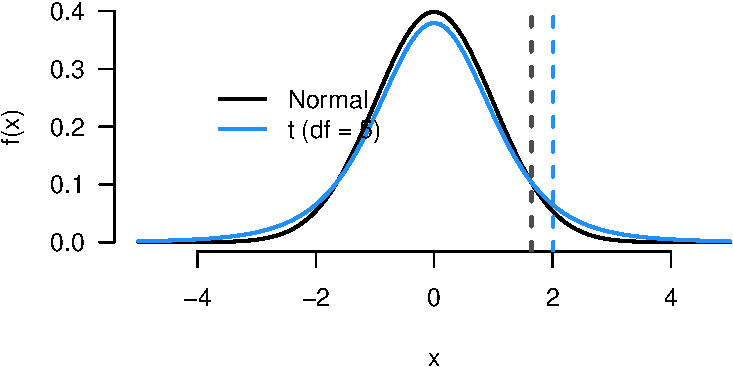
\includegraphics{04_hypothesis_tests_files/figure-pdf/fig-shape-of-t-1.pdf}

}

\caption{\label{fig-shape-of-t}Normal versus t distribution.}

\end{figure}

\hypertarget{confidence-intervals-and-hypothesis-tests}{%
\section{Confidence intervals and hypothesis
tests}\label{confidence-intervals-and-hypothesis-tests}}

At first glance, we may seem sloppy in using \(\alpha\) in deriving a
\(1 - \alpha\) confidence interval in the last chapter and an
\(\alpha\)-level test in this chapter. In reality, we were foreshadowing
the deep connection between the two: every \(1-\alpha\) confidence
interval contains all null hypotheses that we \textbf{would not reject}
with an \(\alpha\)-level test.

This connection is easiest to see with an asymptotically normal
estimator, \(\widehat{\theta}_n\). Consider the hypothesis test of \[ 
H_0: \theta = \theta_0 \quad \text{vs.}\quad H_1: \theta \neq \theta_0,
\] using the test statistic, \[ 
T = \frac{\widehat{\theta}_{n} - \theta_{0}}{\widehat{\se}[\widehat{\theta}_{n}]}. 
\] As we discussed earlier, an \(\alpha = 0.05\) test would reject this
null when \(|T| > 1.96\), or when \[ 
|\widehat{\theta}_{n} - \theta_{0}| > 1.96 \widehat{\se}[\widehat{\theta}_{n}]. 
\] Notice that will be true when \[ 
\theta_{0} < \widehat{\theta}_{n} - 1.96\widehat{\se}[\widehat{\theta}_{n}]\quad \text{ or }\quad \widehat{\theta}_{n} + 1.96\widehat{\se}[\widehat{\theta}_{n}] < \theta_{0}
\] or, equivalently, that null hypothesis is outside of the 95\%
confidence interval,
\[\theta_0 \notin \left[\widehat{\theta}_{n} - 1.96\widehat{\se}[\widehat{\theta}_{n}], \widehat{\theta}_{n} + 1.96\widehat{\se}[\widehat{\theta}_{n}]\right].\]
Of course, our choice of the null hypothesis was arbitrary, which means
that any null hypothesis outside the 95\% confidence interval would be
rejected by a \(\alpha = 0.05\) level test of that null. And any null
hypothesis inside the confidence interval is a null hypothesis that we
would not reject.

This relationship holds more broadly. Any \(1-\alpha\) confidence
interval contains all possible parameter values that would not be
rejected as the null hypothesis of an \(\alpha\)-level hypothesis test.
This connection can be handy for two reasons:

\begin{enumerate}
\def\labelenumi{\arabic{enumi}.}
\tightlist
\item
  We can quickly determine if we would reject a null hypothesis at some
  level by inspecting if it falls in a confidence interval.
\item
  In some situations, determining a confidence interval might be
  difficult, but performing a hypothesis test is straightforward. Then,
  we can find the rejection region for the test and determine what null
  hypotheses would not be rejected at level \(\alpha\) to formulate the
  \(1-\alpha\) confidence interval. We call this process
  \textbf{inverting a test}. A critical application of this method is
  for formulating confidence intervals for treatment effects based on
  randomization inference in the finite population analysis of
  experiments.
\end{enumerate}

\part{Regression}

\hypertarget{sec-regression}{%
\chapter{Linear regression}\label{sec-regression}}

Regression is a tool for assessing the relationship between an
\textbf{outcome variable}, \(Y_i\), and a set of \textbf{covariates},
\(\X_i\). In particular, these tools show how the conditional mean of
\(Y_i\) varies as a function of \(\X_i\). For example, we may want to
know how voting poll wait times vary as a function of some socioeconomic
features of the precinct, like income and racial composition. We usually
accomplish this task by estimating the \textbf{regression function} or
\textbf{conditional expectation function} (CEF) of the outcome given the
covariates, \[
\mu(\bfx) = \E[Y_i \mid \X_i = \bfx].
\] Why are estimation and inference for this regression function
special? Why can't we just use the approaches we have seen for the mean,
variance, covariance, and so on? The fundamental problem with the CEF is
that there may be many, many values \(\bfx\) that can occur and many
different conditional expectations that we will need to estimate. If any
variable in \(\X_i\) is continuous, we must estimate an infinite number
of possible values of \(\mu(\bfx)\). Because it worsens as we add
covariates to \(\X_i\), we refer to this problem as the \textbf{curse of
dimensionality}. How can we resolve this with our measly finite data?

In this chapter, we will explore two ways of ``solving'' the curse of
dimensionality: assuming it away and changing the quantity of interest
to something easier to estimate.

Regression is so ubiquitous in many scientific fields that it has a lot
of acquired notational baggage. In particular, the labels of the \(Y_i\)
and \(\X_i\) vary greatly:

\begin{itemize}
\tightlist
\item
  The outcome can also be called: the response variable, the dependent
  variable, the labels (in machine learning), the left-hand side
  variable, or the regressand.
\item
  The covariates are also called: the explanatory variables, the
  independent variables, the predictors, the regressors, inputs, or
  features.
\end{itemize}

\hypertarget{why-do-we-need-models}{%
\section{Why do we need models?}\label{why-do-we-need-models}}

At first glance, the connection between the CEF and parametric models
might be hazy. For example, imagine we are interested in estimating the
average poll wait times (\(Y_i\)) for Black voters (\(X_i = 1\)) versus
non-Black voters (\(X_i=0\)). In that case, there are two parameters to
estimate, \[
\mu(1) = \E[Y_i \mid X_i = 1] \quad \text{and}\quad \mu(0) = \E[Y_i \mid X_i = 0],
\] which we could estimate by using the plug-in estimators that replace
the population averages with their sample counterparts, \[ 
\widehat{\mu}(1) = \frac{\sum_{i=1}^{n} Y_{i}\mathbb{1}(X_{i} = 1)}{\sum_{i=1}^{n}\mathbb{1}(X_{i} = 1)} \qquad \widehat{\mu}(0) = \frac{\sum_{i=1}^{n} Y_{i}\mathbb{1}(X_{i} = 0)}{\sum_{i=1}^{n}\mathbb{1}(X_{i} = 0)}.
\] These are just the sample averages of the wait times for Black and
non-Black voters, respectively. And because the race variable here is
discrete, we are simply estimating sample means within subpopulations
defined by race. The same logic would apply if we had \(k\) racial
categories: we would have \(k\) conditional expectations to estimate and
\(k\) (conditional) sample means.

Now imagine that we want to know how the average poll wait time varies
as a function of income so that \(X_i\) is (essentially) continuous. Now
we have a different conditional expectation for every possible dollar
amount from 0 to Bill Gates's income. Imagine we pick a particular
income, \$42,238, and so we are interested in the conditional
expectation \(\mu(42,238)= \E[Y_{i}\mid X_{i} = 42,238]\). We could use
the same plug-in estimator in the discrete case, \[
\widehat{\mu}(42,238) = \frac{\sum_{i=1}^{n} Y_{i}\mathbb{1}(X_{i} = 42,238)}{\sum_{i=1}^{n}\mathbb{1}(X_{i} = 42,238)}.
\] What is the problem with this estimator? In all likelihood, no units
in any particular dataset have that exact income, meaning this estimator
is undefined (we would be dividing by zero).

One solution to this problem is to use \textbf{subclassification}, turn
the continuous variable into a discrete one, and proceed with the
discrete approach above. We might group incomes into \$25,000 bins and
then calculate the average wait times of anyone between, say, \$25,000
and \$50,000 income. When we make this estimator switch for practical
purposes, we need to connect it back to the DGP of interest. We could
\textbf{assume} that the CEF of interest only depends on these binned
means, which would mean we have:\\
\[
\mu(x) = 
\begin{cases}
  \E[Y_{i} \mid 0 \leq X_{i} < 25,000] &\text{if } 0 \leq x < 25,000 \\
  \E[Y_{i} \mid 25,000 \leq X_{i} < 50,000] &\text{if } 25,000 \leq x < 50,000\\
  \E[Y_{i} \mid 50,000 \leq X_{i} < 100,000] &\text{if } 50,000 \leq x < 100,000\\
  \vdots \\
  \E[Y_{i} \mid 200,000 \leq X_{i}] &\text{if } 200,000 \leq x\\
\end{cases}
\] This approach assumes, perhaps incorrectly, that the average wait
time does not vary within the bins. Figure~\ref{fig-cef-binned} shows a
hypothetical joint distribution between income and wait times with the
true CEF, \(\mu(x)\), shown in red. The figure also shows the bins
created by subclassification and the implied CEF if we assume
bin-constant means in blue. We can see that the blue function
approximates the true CEF but deviates from it close to the bin edges.
The trade-off is that once we make the assumption, we only have to
estimate one mean for every bin rather than an infinite number of means
for each possible income.

\begin{figure}

{\centering 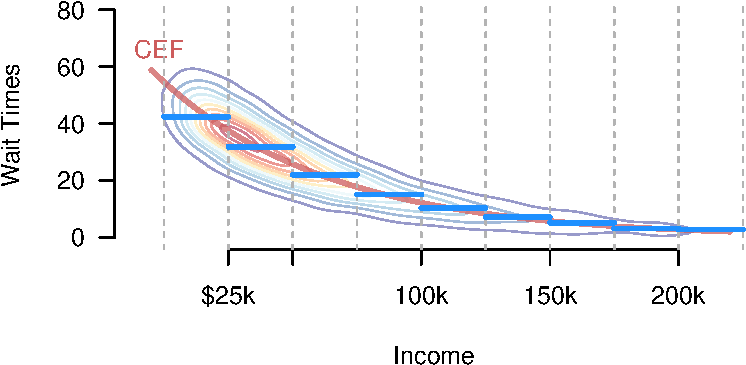
\includegraphics{06_linear_model_files/figure-pdf/fig-cef-binned-1.pdf}

}

\caption{\label{fig-cef-binned}Hypothetical joint distribution of income
and poll wait times (contour plot), conditional expectation function
(red), and the conditional expectation of the binned income (blue).}

\end{figure}

Similarly, we could \textbf{assume} that the CEF follows a simple
functional form like a line, \[ 
\mu(x) = \E[Y_{i}\mid X_{i} = x] = \beta_{0} + \beta_{1} x.
\] This assumption reduces our infinite number of unknowns (the
conditional mean at every possible income) to just two unknowns: the
slope and intercept. As we will see, we can use the standard ordinary
least squares to estimate these parameters. Notice again that if the
true CEF is nonlinear, this assumption is incorrect, and any estimate
based on this assumption might be biased or even inconsistent.

We call the binning and linear assumptions on \(\mu(x)\)
\textbf{functional form} assumptions because they restrict the class of
functions that \(\mu(x)\) can take. While powerful, these types of
assumptions can muddy the roles of defining the quantity of interest and
estimation. If our estimator \(\widehat{\mu}(x)\) performs poorly, it
will be difficult to tell if this is because the estimator is flawed or
our functional form assumptions are incorrect.

To help clarify these issues, we will pursue a different approach:
understanding what linear regression can estimate under minimal
assumptions and then investigating how well this estimand approximates
the true CEF.

\hypertarget{sec-linear-projection}{%
\section{Population linear regression}\label{sec-linear-projection}}

\hypertarget{bivariate-linear-regression}{%
\subsection{Bivariate linear
regression}\label{bivariate-linear-regression}}

Let's set aside the idea of the conditional expectation function and
instead focus on finding the \textbf{linear} function of a single
covariate \(X_i\) that best predicts the outcome. Remember that linear
functions have the form \(a + bX_i\). The \textbf{best linear predictor}
(BLP) or \textbf{population linear regression} of \(Y_i\) on \(X_i\) is
defined as \[ 
m(x) = \beta_0 + \beta_1 x \quad\text{where, }\quad (\beta_{0}, \beta_{1}) = \argmin_{(b_{0}, b_{1}) \in \mathbb{R}^{2}}\; \E[(Y_{i} - b_{0} - b_{1}X_{i} )^{2}].
\] That is, the best linear predictor is the line that results in the
lowest mean-squared error predictions of the outcome given the
covariates, averaging over the joint distribution of the data. This
function is a feature of the joint distribution of the data---the
DGP---and so represents something that we would like to learn about with
our sample. It is an alternative to the CEF for summarizing the
relationship between the outcome and the covariate, though we will see
that they will sometimes be equal. We call \((\beta_{0}, \beta_{1})\)
the \textbf{population linear regression coefficients}. Notice that
\(m(x)\) could differ greatly from the CEF \(\mu(x)\) if the latter is
nonlinear.

We can solve for the best linear predictor using standard calculus
(taking the derivative with respect to each coefficient, setting those
equations equal to 0, and solving the system of equations). The
first-order conditions, in this case, are \[ 
\begin{aligned}
  \frac{\partial \E[(Y_{i} - b_{0} - b_{1}X_{i} )^{2}]}{\partial b_{0}} = \E[-2(Y_{i} - \beta_{0} - \beta_{1}X_{i})] = 0 \\
  \frac{\partial \E[(Y_{i} - b_{0} - b_{1}X_{i} )^{2}]}{\partial b_{1}} = \E[-2(Y_{i} - \beta_{0} - \beta_{1}X_{i})X_{i}] = 0
\end{aligned}  
\] Given the linearity of expectations, it is easy to solve for
\(\beta_0\) in terms of \(\beta_1\), \[ 
\beta_{0} = \E[Y_{i}] - \beta_{1}\E[X_{i}].
\] We can plug this into the first-order condition for \(\beta_1\) to
get \[ 
\begin{aligned}
  0 &= \E[Y_{i}X_{i}] - (\E[Y_{i}] - \beta_{1}\E[X_{i}])\E[X_{i}] - \beta_{1}\E[X_{i}^{2}] \\
    &= \E[Y_{i}X_{i}] - \E[Y_{i}]\E[X_{i}] - \beta_{1}(\E[X_{i}^{2}] - \E[X_{i}]^{2}) \\
    &= \cov(X_{i},Y_{i}) - \beta_{1}\V[X_{i}]\\
  \beta_{1} &= \frac{\cov(X_{i},Y_{i})}{\V[X_{i}]}
\end{aligned}
\]

Thus the slope on the population linear regression of \(Y_i\) on \(X_i\)
is equal to the ratio of the covariance of the two variables divided by
the variance of \(X_i\). From this, we can immediately see that the
covariance will determine the sign of the slope: positive covariances
will lead to positive \(\beta_1\) and negative covariances will lead to
negative \(\beta_1\). In addition, we can see that if \(Y_i\) and
\(X_i\) are independent, \(\beta_1 = 0\). The slope scales this
covariance by the variance of the covariate, so slopes are lower for
more spread-out covariates and higher for more spread-out covariates. If
we define the correlation between these variables as \(\rho_{YX}\), then
we can relate the coefficient to this quantity as \[
\beta_1 = \rho_{YX}\sqrt{\frac{\V[Y_i]}{\V[X_i]}}.
\]

Collecting together our results, we can write the population linear
regression as \[
m(x) = \beta_0 + \beta_1x = \E[Y_i] + \beta_1(x - \E[X_i]),
\] which shows how we adjust our best guess about \(Y_i\) from the mean
of the outcome using the covariate.

It's important to remember that the BLP, \(m(x)\), and the CEF,
\(\mu(x)\), are distinct entities. If the CEF is nonlinear, as in
Figure~\ref{fig-cef-blp}, there will be a difference between these
functions, meaning that the BLP might produce subpar predictions. Below,
we will derive a formal connection between the BLP and the CEF.

\begin{figure}

{\centering 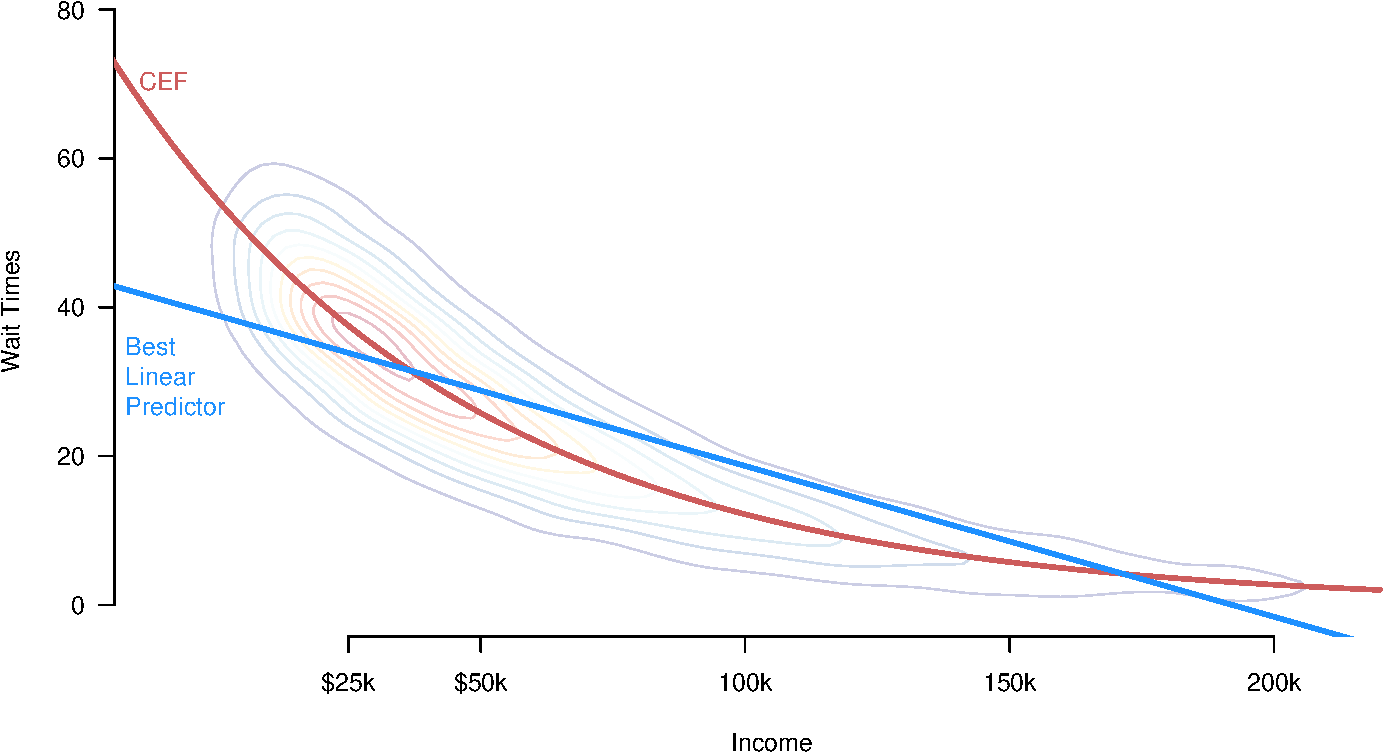
\includegraphics{06_linear_model_files/figure-pdf/fig-cef-blp-1.pdf}

}

\caption{\label{fig-cef-blp}Comparison of the CEF and the best linear
predictor.}

\end{figure}

\hypertarget{beyond-linear-approximations}{%
\subsection{Beyond linear
approximations}\label{beyond-linear-approximations}}

The linear part of the best linear predictor is less restrictive than at
first glance. We can easily modify the minimum MSE problem to find the
best quadratic, cubic, or general polynomial function of \(X_i\) that
predicts \(Y_i\). For example, the quadratic function of \(X_i\) that
best predicts \(Y_i\) would be \[ 
m(X_i, X_i^2) = \beta_0 + \beta_1X_i + \beta_2X_i^2 \quad\text{where}\quad \argmin_{(b_0,b_1,b_2) \in \mathbb{R}^3}\;\E[(Y_{i} - b_{0} - b_{1}X_{i} - b_{2}X_{i}^{2})^{2}].
\] This equation is now a quadratic function of the covariates, but it
is still a linear function of the unknown parameters
\((\beta_{0}, \beta_{1}, \beta_{2})\) so we will call this a best linear
predictor.

We could include higher order terms of \(X_i\) in the same manner, and
as we include more polynomial terms, \(X_i^p\), the more flexible the
function of \(X_i\) we will capture with the BLP. When we estimate the
BLP, however, we usually will pay for this flexibility in terms of
overfitting and high variance in our estimates.

\hypertarget{linear-prediction-with-multiple-covariates}{%
\subsection{Linear prediction with multiple
covariates}\label{linear-prediction-with-multiple-covariates}}

We now generalize the idea of a best linear predictor to a setting with
an arbitrary number of covariates. In this setting, remember that the
linear function will be

\[ 
\bfx'\bfbeta = x_{1}\beta_{1} + x_{2}\beta_{2} + \cdots + x_{k}\beta_{k}.
\] We will define the \textbf{best linear predictor} (BLP) to be \[ 
m(\bfx) = \bfx'\bfbeta, \quad \text{where}\quad \bfbeta = \argmin_{\mb{b} \in \real^k}\; \E\bigl[ \bigl(Y_{i} - \mb{X}_{i}'\mb{b} \bigr)^2\bigr]
\]

This BLP solves the same fundamental optimization problem as in the
bivariate case: it chooses the set of coefficients that minimizes the
mean-squared error averaging over the joint distribution of the data.

\begin{tcolorbox}[enhanced jigsaw, colbacktitle=quarto-callout-note-color!10!white, colframe=quarto-callout-note-color-frame, arc=.35mm, left=2mm, toptitle=1mm, rightrule=.15mm, title=\textcolor{quarto-callout-note-color}{\faInfo}\hspace{0.5em}{Best linear projection assumptions}, colback=white, leftrule=.75mm, toprule=.15mm, coltitle=black, opacityback=0, breakable, bottomtitle=1mm, titlerule=0mm, bottomrule=.15mm, opacitybacktitle=0.6]

Without some assumptions on the joint distribution of the data, the
following ``regularity conditions'' will ensure the existence of the
BLP:

\begin{enumerate}
\def\labelenumi{\arabic{enumi}.}
\tightlist
\item
  \(\E[Y^2] < \infty\) (outcome has finite mean/variance)
\item
  \(\E\Vert \mb{X} \Vert^2 < \infty\) (\(\mb{X}\) has finite
  means/variances/covariances)
\item
  \(\mb{Q}_{\mb{XX}} = \E[\mb{XX}']\) is positive definite (columns of
  \(\X\) are linearly independent)\\
\end{enumerate}

\end{tcolorbox}

Under these assumptions, it is possible to derive a closed-form
expression for the \textbf{population coefficients} \(\bfbeta\) using
matrix calculus. To set up the optimization problem, we will find the
first-order condition by taking the derivative of the expectation of the
squared errors. First, let's take the derivative of the squared
prediction errors using the chain rule: \[ 
\begin{aligned}
  \frac{\partial}{\partial \mb{b}}\left(Y_{i} - \X_{i}'\mb{b}\right)^{2}
  &= 2\left(Y_{i} - \X_{i}'\mb{b}\right)\frac{\partial}{\partial \mb{b}}(Y_{i} - \X_{i}'\mb{b}) \\
  &= -2\left(Y_{i} - \X_{i}'\mb{b}\right)\X_{i} \\
  &= -2\X_{i}\left(Y_{i} - \X_{i}'\mb{b}\right) \\
  &= -2\left(\X_{i}Y_{i} - \X_{i}\X_{i}'\mb{b}\right),
\end{aligned}
\] where the third equality comes from the fact that
\((Y_{i} - \X_{i}'\bfbeta)\) is a scalar. We can now plug this into the
expectation to get the first-order condition and solve for \(\bfbeta\),
\[ 
\begin{aligned}
  0 &= -2\E[\X_{i}Y_{i} - \X_{i}\X_{i}'\bfbeta ] \\
  \E[\X_{i}\X_{i}'] \bfbeta &= \E[\X_{i}Y_{i}],
\end{aligned}
\] which implies the population coefficients are \[ 
\bfbeta = \left(\E[\X_{i}\X_{i}']\right)^{-1}\E[\X_{i}Y_{i}] = \mb{Q}_{\mb{XX}}^{-1}\mb{Q}_{\mb{X}Y}
\] We now have an expression for the coefficients for the population
best linear predictor in terms of the joint distribution
\((Y_{i}, \X_{i})\). A couple of facts might be useful for reasoning
this expression. Recall that \(\mb{Q}_{\mb{XX}} = \E[\X_{i}\X_{i}']\) is
a \(k\times k\) matrix and \(\mb{Q}_{\X Y} = \E[\X_{i}Y_{i}]\) is a
\(k\times 1\) column vector, which implies that \(\bfbeta\) is also a
\(k \times 1\) column vector.

\begin{tcolorbox}[enhanced jigsaw, colbacktitle=quarto-callout-note-color!10!white, colframe=quarto-callout-note-color-frame, arc=.35mm, left=2mm, toptitle=1mm, rightrule=.15mm, title=\textcolor{quarto-callout-note-color}{\faInfo}\hspace{0.5em}{Note}, colback=white, leftrule=.75mm, toprule=.15mm, coltitle=black, opacityback=0, breakable, bottomtitle=1mm, titlerule=0mm, bottomrule=.15mm, opacitybacktitle=0.6]

Intuitively, what is happening in the expression for the population
regression coefficients? It is helpful to separate the intercept or
constant term so that we have \[ 
Y_{i} = \beta_{0} + \X'\bfbeta + e_{i},
\] so \(\bfbeta\) refers to just the vector of coefficients for the
covariates. In this case, we can write the coefficients in a more
interpretable way: \[ 
\bfbeta = \V[\X]^{-1}\text{Cov}(\X, Y), \qquad \beta_0 = \mu_Y - \mb{\mu}'_{\mb{X}}\bfbeta
\]

Thus, the population coefficients take the covariance between the
outcome and the covariates and ``divide'' it by information about
variances and covariances of the covariates. The intercept recenters the
regression so that projection errors are mean zero. Thus, we can see
that these coefficients generalize the bivariate formula to this
multiple covariate context.

\end{tcolorbox}

With an expression for the population linear regression coefficients, we
can write the linear projection as \[ 
m(\X_{i}) = \X_{i}'\left(\E[\X_{i}\X_{i}']\right)^{-1}\E[\X_{i}Y_{i}] = \X_{i}'\mb{Q}_{\mb{XX}}^{-1}\mb{Q}_{\mb{X}Y}
\]

\hypertarget{projection-error}{%
\subsection{Projection error}\label{projection-error}}

The \textbf{projection error} is the difference between the actual value
of \(Y_i\) and the projection, \[ 
e_{i} = Y_{i} - m(\X_{i}) = Y_i - \X_{i}'\bfbeta,
\] where we have made no assumptions about this error yet. The
projection error is simply the prediction error of the best linear
prediction. Rewriting this definition, we can see that we can always
write the outcome as the linear projection plus the projection error,
\[ 
Y_{i} = \X_{i}'\bfbeta + e_{i}.
\] Notice that this looks suspiciously similar to a linearity assumption
on the CEF, but we haven't made any assumptions here. Instead, we have
just used the definition of the projection error to write a tautological
statement: \[ 
Y_{i} = \X_{i}'\bfbeta + e_{i} = \X_{i}'\bfbeta + Y_{i} - \X_{i}'\bfbeta = Y_{i}.
\] The critical difference between this representation and the usual
linear model assumption is what properties \(e_{i}\) possesses.

One key property of the projection errors is that when the covariate
vector includes an ``intercept'' or constant term, the projection errors
are uncorrelated with the covariates. To see this, we first note that
\(\E[\X_{i}e_{i}] = 0\) since \[ 
\begin{aligned}
  \E[\X_{i}e_{i}] &= \E[\X_{{i}}(Y_{i} - \X_{i}'\bfbeta)] \\
                  &= \E[\X_{i}Y_{i}] - \E[\X_{i}\X_{i}']\bfbeta \\
                  &= \E[\X_{i}Y_{i}] - \E[\X_{i}\X_{i}']\left(\E[\X_{i}\X_{i}']\right)^{-1}\E[\X_{i}Y_{i}] \\
  &= \E[\X_{i}Y_{i}] - \E[\X_{i}Y_{i}] = 0
\end{aligned}
\] Thus, for every \(X_{ij}\) in \(\X_{i}\), we have
\(\E[X_{ij}e_{i}] = 0\). If one of the entries in \(\X_i\) is a constant
1, then this also implies that \(\E[e_{i}] = 0\). Together, these facts
imply that the projection error is uncorrelated with each \(X_{ij}\),
since \[ 
\cov(X_{ij}, e_{i}) = \E[X_{ij}e_{i}] - \E[X_{ij}]\E[e_{i}] = 0 - 0 = 0
\] Notice that we still have made no assumptions about these projection
errors except for some mild regularity conditions on the joint
distribution of the outcome and covariates. Thus, in very general
settings, we can write the linear projection model
\(Y_i = \X_i'\bfbeta + e_i\) where
\(\bfbeta = \left(\E[\X_{i}\X_{i}']\right)^{-1}\E[\X_{i}Y_{i}]\) and
conclude that \(\E[\X_{i}e_{i}] = 0\) by definition, not by assumption.

The projection error is uncorrelated with the covariates, so does this
mean that the CEF is linear? Unfortunately, no. Recall that while
independence implies uncorrelated, the reverse does not hold. So when we
look at the CEF, we have \[ 
\E[Y_{i} \mid \X_{i}] = \X_{i}'\bfbeta + \E[e_{i} \mid \X_{i}],
\] and the last term \(\E[e_{i} \mid \X_{i}]\) would only be 0 if the
errors were independent of the covariates, so
\(\E[e_{i} \mid \X_{i}] = \E[e_{i}] = 0\). But nowhere in the linear
projection model did we assume this. So while we can (almost) always
write the outcome as \(Y_i = \X_i'\bfbeta + e_i\) and have those
projection errors be uncorrelated with the covariates, it will require
additional assumptions to ensure that the true CEF is, in fact, linear
\(\E[Y_{i} \mid \X_{i}] = \X_{i}'\bfbeta\).

Let's take a step back. What have we shown here? In a nutshell, we have
shown that a population linear regression exists under very general
conditions, and we can write the coefficients of that population linear
regression as a function of expectations of the joint distribution of
the data. We did not assume that the CEF was linear nor that the
projection errors were normal.

Why do we care about this? The ordinary least squares estimator, the
workhorse regression estimator, targets this quantity of interest in
large samples, regardless of whether the true CEF is linear or not.
Thus, even when a linear CEF assumption is incorrect, OLS still targets
a perfectly valid quantity of interest: the coefficients from this
population linear projection.

\hypertarget{linear-cefs-without-assumptions}{%
\section{Linear CEFs without
assumptions}\label{linear-cefs-without-assumptions}}

What is the relationship between the best linear predictor (which we
just saw generally exists) and the CEF? To draw the connection, remember
a vital property of the conditional expectation: it is the function of
\(\X_i\) that best predicts \(Y_{i}\). The population regression was the
best \textbf{linear} predictor, but the CEF is the best predictor among
all nicely behaved functions of \(\X_{i}\), linear or nonlinear. In
particular, if we label \(L_2\) to be the set of all functions of the
covariates \(g()\) that have finite squared expectation,
\(\E[g(\X_{i})^{2}] < \infty\), then we can show that the CEF has the
lowest squared prediction error in this class of functions: \[ 
\mu(\X) = \E[Y_{i} \mid \X_{i}] = \argmin_{g(\X_i) \in L_2}\; \E\left[(Y_{i} - g(\X_{i}))^{2}\right],
\]

So we have established that the CEF is the best predictor and the
population linear regression \(m(\X_{i})\) is the best linear predictor.
These two facts allow us to connect the CEF and the population
regression.

\begin{theorem}[]\protect\hypertarget{thm-cef-blp}{}\label{thm-cef-blp}

If \(\mu(\X_{i})\) is a linear function of \(\X_i\), then
\(\mu(\X_{i}) = m(\X_{i}) = \X_i'\bfbeta\).

\end{theorem}

This theorem says that if the true CEF is linear, it equals the
population linear regression. The proof of this is straightforward: the
CEF is the best predictor, so if it is linear, it must also be the best
linear predictor.

In general, we are in the business of learning about the CEF, so we are
unlikely to know if it genuinely is linear or not. In some situations,
however, we can show that the CEF is linear without any additional
assumptions. These will be situations when the covariates take on a
finite number of possible values. Suppose we are interested in the CEF
of poll wait times for Black (\(X_i = 1\)) vs.~non-Black (\(X_i = 0\))
voters. In this case, there are two possible values of the CEF,
\(\mu(1) = \E[Y_{i}\mid X_{i}= 1]\), the average wait time for Black
voters, and \(\mu(0) = \E[Y_{i}\mid X_{i} = 0]\), the average wait time
for non-Black voters. Notice that we can write the CEF as \[ 
\mu(x) = x \mu(1) + (1 - x) \mu(0) = \mu(0) + x\left(\mu(1) - \mu(0)\right)= \beta_0 + x\beta_1,
\] which is clearly a linear function of \(x\). Based on this
derivation, we can see that the coefficients of this linear CEF have a
clear interpretation:

\begin{itemize}
\tightlist
\item
  \(\beta_0 = \mu(0)\): the expected wait time for a Black voter.
\item
  \(\beta_1 = \mu(1) - \mu(0)\): the difference in average wait times
  between Black and non-Black voters. Notice that it matters how
  \(X_{i}\) is defined here since the intercept will always be the
  average outcome when \(X_i = 0\), and the slope will always be the
  difference in means between the \(X_i = 1\) group and the \(X_i = 0\)
  group.
\end{itemize}

What about a categorical covariate with more than two levels? For
instance, we might be interested in wait times by party identification,
where \(X_i = 1\) indicates Democratic voters, \(X_i = 2\) indicates
Republican voters, and \(X_i = 3\) indicates independent voters. How can
we write the CEF of wait times as a linear function of this variable?
That would assume that the difference between Democrats and Republicans
is the same as for Independents and Republicans. With more than two
levels, we can represent a categorical variable as a vector of binary
variables, \(\X_i = (X_{i1}, X_{i2})\), where \[ 
\begin{aligned}
  X_{{i1}} &= \begin{cases}
                1&\text{if Republican} \\
                   0 & \text{if not Republican}
              \end{cases} \\
X_{{i2}} &= \begin{cases}
                1&\text{if independent} \\
                   0 & \text{if not independent}
              \end{cases} \\
\end{aligned}
\] These two indicator variables encode the same information as the
original three-level variable, \(X_{i}\). If I know the values of
\(X_{i1}\) and \(X_{i2}\), I know exactly what party to which \(i\)
belongs. Thus, the CEFs for \(X_i\) and the pair of indicator variables,
\(\X_i\), are precisely the same, but the latter admits a lovely linear
representation, \[
\E[Y_i \mid X_{i1}, X_{i2}] = \beta_0 + \beta_1 X_{i1} + \beta_2 X_{i2},
\] where

\begin{itemize}
\tightlist
\item
  \(\beta_0 = \E[Y_{i} \mid X_{i1} = 0, X_{i2} = 0]\) is the average
  wait time for the group who does not get an indicator variable
  (Democrats in this case).
\item
  \(\beta_1 = \E[Y_{i} \mid X_{i1} = 1, X_{i2} = 0] - \E[Y_{i} \mid X_{i1} = 0, X_{i2} = 0]\)
  is the difference in means between Republican voters and Democratic
  voters, or the difference between the first indicator group and the
  baseline group.
\item
  \(\beta_2 = \E[Y_{i} \mid X_{i1} = 0, X_{i2} = 1] - \E[Y_{i} \mid X_{i1} = 0, X_{i2} = 0]\)
  is the difference in means between independent voters and Democratic
  voters, or the difference between the second indicator group and the
  baseline group.
\end{itemize}

This approach easily generalizes to categorical variables with an
arbitrary number of levels.

What have we shown? The CEF will be linear without additional
assumptions when there is a categorical covariate. We can show that this
continues to hold even when we have multiple categorical variables. We
now have two binary covariates: \(X_{i1}=1\) indicating a Black voter,
and \(X_{i2} = 1\) indicating an urban voter. With these two binary
variables, there are four possible values of the CEF: \[ 
\mu(x_1, x_2) = \begin{cases} 
 \mu_{00} & \text{if } x_1 = 0 \text{ and } x_2 = 0 \text{ (non-Black, rural)} \\
 \mu_{10} & \text{if } x_1 = 1 \text{ and } x_2 = 0 \text{ (Black, rural)} \\
 \mu_{01} & \text{if } x_1 = 0 \text{ and } x_2 = 1 \text{ (non-Black, urban)} \\
 \mu_{11} & \text{if } x_1 = 1 \text{ and } x_2 = 1 \text{ (Black, urban)}
 \end{cases}
\] We can write this as \[ 
\mu(x_{1}, x_{2}) = (1 - x_{1})(1 - x_{2})\mu_{00} + x_{1}(1 -x_{2})\mu_{10} + (1-x_{1})x_{2}\mu_{01} + x_{1}x_{2}\mu_{11},
\] which we can rewrite as \[ 
\mu(x_1, x_2) = \beta_0 + x_1\beta_1 + x_2\beta_2 + x_1x_2\beta_3,
\] where

\begin{itemize}
\tightlist
\item
  \(\beta_0 = \mu_{00}\): average wait times for rural non-Black voters.
\item
  \(\beta_1 = \mu_{10} - \mu_{00}\): difference in means for rural Black
  vs.~rural non-Black voters.
\item
  \(\beta_2 = \mu_{01} - \mu_{00}\): difference in means for urban
  non-Black vs.~rural non-Black voters.
\item
  \(\beta_3 = (\mu_{11} - \mu_{01}) - (\mu_{10} - \mu_{00})\):
  difference in urban racial difference vs rural racial difference.
\end{itemize}

Thus, we can write the CEF with two binary covariates as linear when the
linear specification includes a multiplicative interaction between them
(\(x_1x_2\)). This result holds for all pairs of binary covariates, and
we can generalize the interpretation of the coefficients in the CEF as

\begin{itemize}
\tightlist
\item
  \(\beta_0 = \mu_{00}\): average outcome when both variables are 0.
\item
  \(\beta_1 = \mu_{10} - \mu_{00}\): difference in average outcomes for
  the first covariate when the second covariate is 0.
\item
  \(\beta_2 = \mu_{01} - \mu_{00}\): difference in average outcomes for
  the second covariate when the first covariate is 0.
\item
  \(\beta_3 = (\mu_{11} - \mu_{01}) - (\mu_{10} - \mu_{00})\): change in
  the ``effect'' of the first (second) covariate when the second (first)
  covariate goes from 0 to 1.
\end{itemize}

This result also generalizes to an arbitrary number of binary
covariates. If we have \(p\) binary covariates, then the CEF will be
linear with all two-way interactions, \(x_1x_2\), all three-way
interactions, \(x_1x_2x_3\), up to the \(p\)-way interaction
\(x_1\times\cdots\times x_p\). Furthermore, we can generalize to
arbitrary numbers of categorical variables by expanding each into a
series of binary variables and then including all interactions between
the resulting binary variables.

We have established that when we have a set of categorical covariates,
the true CEF will be linear, and we have seen the various ways to
represent that CEF. Notice that when we use, for example, ordinary least
squares, we are free to choose how to include our variables. That means
that we could run a regression of \(Y_i\) on \(X_{i1}\) and \(X_{i2}\)
without an interaction term. This model will only be correct if
\(\beta_3\) is equal to 0, and so the interaction term is irrelevant.
Because of this ability to choose our models, it's helpful to have a
language for models that capture the linear CEF appropriately. We call a
model \textbf{saturated} if there are as many coefficients as the CEF's
unique values. A saturated model, by its nature, can always be written
as a linear function without assumptions. The above examples show how to
construct saturated models in various situations.

\hypertarget{interpretation-of-the-regression-coefficients}{%
\section{Interpretation of the regression
coefficients}\label{interpretation-of-the-regression-coefficients}}

We have seen how to interpret population regression coefficients when
the CEF is linear without assumptions. How do we interpret the
population coefficients \(\bfbeta\) in other settings?

Let's start with the simplest case, where every entry in \(\X_{i}\)
represents a different covariate and no covariate is any function of
another (we'll see why this caveat is necessary below). In this simple
case, the \(k\)th coefficient, \(\beta_{k}\), will represent the change
in the predicted outcome for a one-unit change in the \(k\)th covariate
\(X_{ik}\), holding all other covariates fixed. We can see this from \[ 
\begin{aligned}
  m(x_{1} + 1, x_{2}) & = \beta_{0} + \beta_{1}(x_{1} + 1) + \beta_{2}x_{2} \\
  m(x_{1}, x_{2}) &= \beta_{0} + \beta_{1}x_{1} + \beta_{2}x_{2},
\end{aligned} 
\] so that the change in the predicted outcome for increasing \(X_{i1}\)
by one unit is \[
 m(x_{1} + 1, x_{2}) - m(x_{1}, x_{2}) = \beta_1
\] Notice that nothing changes in this interpretation if we add more
covariates to the vector, \[
 m(x_{1} + 1, \bfx_{2}) - m(x_{1}, \bfx_{2}) = \beta_1,
\] the coefficient on a particular variable is the change in the
predicted outcome for a one-unit change in the covariate holding all
other covariates constant. Each coefficient summarizes the ``all else
equal'' difference in the predicted outcome for each covariate.

\hypertarget{polynomial-functions-of-the-covariates}{%
\subsection{Polynomial functions of the
covariates}\label{polynomial-functions-of-the-covariates}}

The interpretation of the population regression coefficients becomes
more complicated when we include nonlinear functions of the covariates.
In that case, multiple coefficients control how a change in a covariate
will change the predicted value of \(Y_i\). Suppose that we have a
quadratic function of \(X_{i1}\), \[ 
m(x_1, x_1^2, x_{2}) = \beta_{0} + \beta_{1}x_{1} + \beta_{2}x_{1}^{2} + \beta_{3}x_{2},
\] and try to look at a one-unit change in \(x_1\), \[ 
\begin{aligned}
  m(x_{1} + 1, (x_{1} + 1)^{2}, x_{2}) & = \beta_{0} + \beta_{1}(x_{1} + 1) + \beta_{2}(x_{1} + 1)^{2}+ \beta_{3}x_{2} \\
  m(x_{1}, x_{1}^{2}, x_{2}) &= \beta_{0} + \beta_{1}x_{1} + \beta_{2}x_{1}^{2} + \beta_{3}x_{2},
\end{aligned} 
\] resulting in \(\beta_1 + \beta_2(2x_{1} + 1)\). This formula might be
an interesting quantity, but we will more commonly use the derivative of
\(m(\bfx)\) with respect to \(x_1\) as a measure of the marginal effect
of \(X_{i1}\) on the predicted value of \(Y_i\) (holding all other
variables constant), where ``marginal'' here means the change in
prediction for a very small change in \(X_{i1}\).\footnote{Notice the
  choice of language here. The marginal effect is on the predicted value
  of \(Y_i\), not on \(Y_i\) itself. So these marginal effects are
  associational, not necessarily causal quantities.} In the case of the
quadratic covariate, we have \[ 
\frac{\partial m(x_{1}, x_{1}^{2}, x_{2})}{\partial x_{1}} = \beta_{1} + 2\beta_{2}x_{1},
\] so the marginal effect on prediction varies as a function of \(x_1\).
From this, we can see that the individual interpretations of the
coefficients are less interesting: \(\beta_1\) is the marginal effect
when \(X_{i1} = 0\) and \(\beta_2 / 2\) describes how a one-unit change
in \(X_{i1}\) changes the marginal effect. As is hopefully clear, it
will often be more straightforward to visualize the nonlinear predictor
function (perhaps using the orthogonalization techniques in
Section~\ref{sec-fwl}).

\hypertarget{interactions}{%
\subsection{Interactions}\label{interactions}}

Another common nonlinear function of the covariates is when we include
\textbf{interaction terms} or covariates that are products of two other
covariates, \[ 
m(x_{1}, x_{2}, x_{1}x_{2}) = \beta_{0} + \beta_{1}x_{1} + \beta_{2}x_{2} + \beta_{3}x_{1}x_{2}.
\] In these situations, we can also use the derivative of the BLP to
measure the marginal effect of one variable or the other on the
predicted value of \(Y_i\). In particular, we have \[ 
\begin{aligned}
  \frac{\partial m(x_{1}, x_{2}, x_{1}x_{2})}{\partial x_1} &= \beta_1 + \beta_3x_2, \\
  \frac{\partial m(x_{1}, x_{2}, x_{1}x_{2})}{\partial x_2} &= \beta_2 + \beta_3x_1.
\end{aligned}
\] Here, the coefficients are slightly more interpretable:

\begin{itemize}
\tightlist
\item
  \(\beta_1\): the marginal effect of \(X_{i1}\) on predicted \(Y_i\)
  when \(X_{i2} = 0\).
\item
  \(\beta_2\): the marginal effect of \(X_{i2}\) on predicted \(Y_i\)
  when \(X_{i1} = 0\).
\item
  \(\beta_3\): the change in the marginal effect of \(X_{i1}\) due to a
  one-unit change in \(X_{i2}\) \textbf{OR} the change in the marginal
  effect of \(X_{i2}\) due to a one-unit change in \(X_{i1}\).
\end{itemize}

If we add more covariates to this BLP, these interpretations change to
``holding all other covariates constant.''

Interactions are a routine part of social science research because they
allow us to assess how the relationship between the outcome and an
independent variable varies by the values of another variable. In the
context of our study of voter wait times, if \(X_{i1}\) is income and
\(X_{i2}\) is the Black/non-Black voter indicator, then \(\beta_3\)
represents the change in the slope of the wait time-income relationship
between Black and non-Black voters.

\hypertarget{sec-fwl}{%
\section{Multiple regression from bivariate regression}\label{sec-fwl}}

When we have a regression of an outcome on two covariates, it is helpful
to understand how the coefficients of one variable relate to the other.
For example, if we have the following best linear projection:
\begin{equation}\protect\hypertarget{eq-two-var-blp}{}{ 
(\alpha, \beta, \gamma) = \argmin_{(a,b,c) \in \mathbb{R}^{3}} \; \E[(Y_{i} - (a + bX_{i} + cZ_{i}))^{2}]
}\label{eq-two-var-blp}\end{equation} Is there some way to understand
the \(\beta\) coefficient here regarding simple linear regression? As it
turns out, yes. From the above results, we know that the intercept has a
simple form: \[
\alpha = \E[Y_i] - \beta\E[X_i] - \gamma\E[Z_i].
\] Let's investigate the first order condition for \(\beta\): \[ 
\begin{aligned}
  0 &= \E[Y_{i}X_{i}] - \alpha\E[X_{i}] - \beta\E[X_{i}^{2}] - \gamma\E[X_{i}Z_{i}] \\
    &= \E[Y_{i}X_{i}] - \E[Y_{i}]\E[X_{i}] + \beta\E[X_{i}]^{2} + \gamma\E[X_{i}]\E[Z_{i}] - \beta\E[X_{i}^{2}] - \gamma\E[X_{i}Z_{i}] \\
  &= \cov(Y, X) - \beta\V[X_{i}] - \gamma \cov(X_{i}, Z_{i})
\end{aligned}
\] We can see from this that if \(\cov(X_{i}, Z_{i}) = 0\), then the
coefficient on \(X_i\) will be the same as in the simple regression
case, \(\cov(Y_{i}, X_{i})/\V[X_{i}]\). When \(X_i\) and \(Z_i\) are
uncorrelated, we sometimes call them \textbf{orthogonal}.

To write a simple formula for \(\beta\) when the covariates are not
orthogonal, we will \textbf{orthogonalize} \(X_i\) by obtaining the
prediction errors from a population linear regression of \(X_i\) on
\(Z_i\): \[ 
\widetilde{X}_{i} = X_{i} - (\delta_{0} + \delta_{1}Z_{i}) \quad\text{where}\quad (\delta_{0}, \delta_{1}) = \argmin_{(d_{0},d_{1}) \in \mathbb{R}^{2}} \; \E[(X_{i} - (d_{0} + d_{1}Z_{i}))^{2}]
\] Given the properties of projection errors, we know that this
orthogonalized version of \(X_{i}\) will be uncorrelated with \(Z_{i}\)
since \(\E[\widetilde{X}_{i}Z_{i}] = 0\). Remarkably, the coefficient on
\(X_i\) from the ``long'' BLP in Equation~\ref{eq-two-var-blp} is the
same as the regression of \(Y_i\) on this orthogonalized
\(\widetilde{X}_i\), \[ 
\beta = \frac{\text{cov}(Y_{i}, \widetilde{X}_{i})}{\V[\widetilde{X}_{i}]}
\]

We can expand this idea to when there are several other covariates.
Suppose now that we are interested in a regression of \(Y_i\) on
\(\X_i\) and we are interested in the coefficient on the \(k\)th
covariate. Let \(\X_{i,-k}\) be the vector of covariates omitting the
\(k\)th entry and let \(m_k(\X_{i,-k})\) represent the BLP of \(X_{ik}\)
on these other covariates. We can define
\(\widetilde{X}_{ik} = X_{ik} - m_{k}(\X_{i,-k})\) as the \(k\)th
variable orthogonalized with respect to the rest of the variables and we
can write the coefficient on \(X_{ik}\) as \[ 
\beta_k = \frac{\cov(Y_i, \widetilde{X}_{ik})}{\V[\widetilde{X}_{ik}]}.
\] Thus, the population regression coefficient in the BLP is the same as
from a bivariate regression of the outcome on the projection error for
\(X_{ik}\) projected on all other covariates. One interpretation of
coefficients in a population multiple regression is they represent the
relationship between the outcome and the covariate after removing the
linear relationships of all other variables.

\hypertarget{omitted-variable-bias}{%
\section{Omitted variable bias}\label{omitted-variable-bias}}

In many situations, we might need to choose whether to include a
variable in a regression or not, so it can be helpful to understand how
this choice might affect the population coefficients on the other
variables in the regression. Suppose we have a variable \(Z_i\) that we
may add to our regression which currently has \(\X_i\) as the
covariates. We can write this new projection as \[ 
m(\X_i, Z_i) = \X_i'\bfbeta + Z_i\gamma, \qquad m(\X_{i}) = \X_i'\bs{\delta},
\] where we often refer to \(m(\X_i, Z_i)\) as the long regression and
\(m(\X_i)\) as the short regression.

We know from the definition of the BLP that we can write the short
coefficients as \[ 
\bs{\delta} = \left(\E[\X_{i}\X_{i}']\right)^{-1} \E[\X_{i}Y_{i}].
\] Letting \(e_i = Y_i - m(\X_{i}, Z_{i})\) be the projection errors
from the long regression, we can write this as \[ 
\begin{aligned}
  \bs{\delta} &= \left(\E[\X_{i}\X_{i}']\right)^{-1} \E[\X_{i}(\X_{i}'\bfbeta + Z_{i}\gamma + e_{i})] \\
              &= \left(\E[\X_{i}\X_{i}']\right)^{-1}(\E[\X_{i}\X_{i}']\bfbeta + \E[\X_{i}Z_{i}]\gamma + \E[\X_{i}e_{i}]) \\
              &= \bfbeta + \left(\E[\X_{i}\X_{i}']\right)^{-1}\E[\X_{i}Z_{i}]\gamma
\end{aligned}
\] Notice that the vector in the second term is the linear projection
coefficients of a population linear regression of \(Z_i\) on the
\(\X_i\). If we call these coefficients \(\bs{\pi}\), then the short
coefficients are \[ 
\bs{\delta} = \bfbeta + \bs{\pi}\gamma. 
\]

We can rewrite this to show that the difference between the coefficients
in these two projections is \(\bs{\delta} - \bfbeta= \bs{\pi}\gamma\) or
the product of the coefficient on the ``excluded'' \(Z_i\) and the
coefficient of the included \(\X_i\) on the excluded. Most textbooks
refer to this difference as the \textbf{omitted variable bias} of
omitting \(Z_i\) under the idea that \(\bfbeta\) is the true target of
inference. But the result is much broader than this since it just tells
us how to relate the coefficients of two nested projections.

The last two results (multiple regressions from bivariate and omitted
variable bias) are sometimes presented as results for the ordinary least
squares estimator that we will show in the next chapter. We introduce
them here as features of a particular population quantity, the linear
projection or population linear regression.

\hypertarget{drawbacks-of-the-blp}{%
\section{Drawbacks of the BLP}\label{drawbacks-of-the-blp}}

The best linear predictor is, of course, a \emph{linear} approximation
to the CEF, and this approximation could be quite poor if the true CEF
is highly nonlinear. A more subtle issue with the BLP is that it is
sensitive to the marginal distribution of the covariates when the CEF is
nonlinear. Let's return to our example of voter wait times and income.
In Figure~\ref{fig-blp-limits}, we show the true CEF and the BLP when we
restrict income below \$50,000 or above \$100,000. The BLP can vary
quite dramatically here. This figure is an extreme example, but the
essential point will still hold as the marginal distribution of \(X_i\)
changes.

\begin{figure}

{\centering 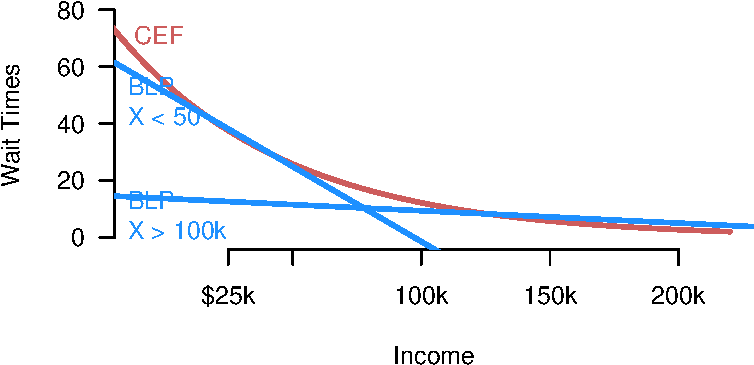
\includegraphics{06_linear_model_files/figure-pdf/fig-blp-limits-1.pdf}

}

\caption{\label{fig-blp-limits}Linear projections for when truncating
income distribution below \$50k and above \$100k.}

\end{figure}

\hypertarget{sec-ols-mechanics}{%
\chapter{The mechanics of least squares}\label{sec-ols-mechanics}}

This chapter explores the most widely used estimator for population
linear regressions: \textbf{ordinary least squares} (OLS). OLS is a
plug-in estimator for the best linear projection (or population linear
regression) described in the last chapter. Its popularity is partly due
to its ease of interpretation, computational simplicity, and statistical
efficiency.

In this chapter, we focus on motivating the estimator and the mechanical
or algebraic properties of the OLS estimator. In the next chapter, we
will investigate its statistical assumptions. Textbooks often introduce
OLS under an assumption of a linear model for the conditional
expectation, but this is unnecessary if we view the inference target as
the best linear predictor. We discuss this point more fully in the next
chapter.

\begin{figure}

{\centering 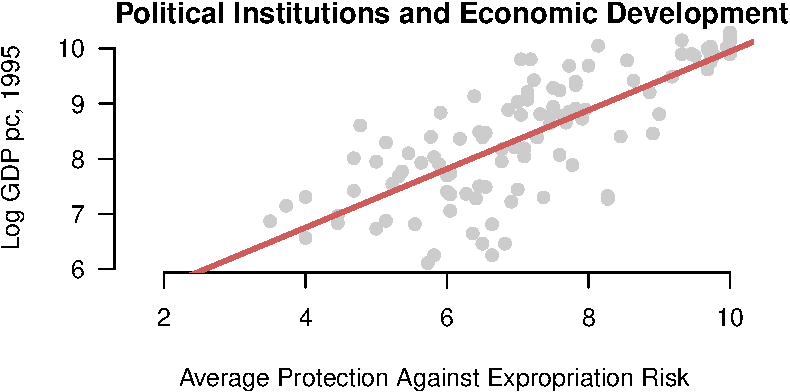
\includegraphics{07_least_squares_files/figure-pdf/fig-ajr-scatter-1.pdf}

}

\caption{\label{fig-ajr-scatter}Relationship between political
institutions and economic development from Acemoglu, Johnson, and
Robinson (2001).}

\end{figure}

\hypertarget{deriving-the-ols-estimator}{%
\section{Deriving the OLS estimator}\label{deriving-the-ols-estimator}}

In the last chapter on the linear model and the best linear projection,
we operated purely in the population, not samples. We derived the
population regression coefficients \(\bfbeta\), representing the
coefficients on the line of best fit in the population. We now take
these as our quantity of interest.

\begin{tcolorbox}[enhanced jigsaw, colbacktitle=quarto-callout-note-color!10!white, colframe=quarto-callout-note-color-frame, arc=.35mm, left=2mm, toptitle=1mm, rightrule=.15mm, title=\textcolor{quarto-callout-note-color}{\faInfo}\hspace{0.5em}{Assumption}, colback=white, leftrule=.75mm, toprule=.15mm, coltitle=black, opacityback=0, breakable, bottomtitle=1mm, titlerule=0mm, bottomrule=.15mm, opacitybacktitle=0.6]

The variables
\(\{(Y_1, \X_1), \ldots, (Y_i,\X_i), \ldots, (Y_n, \X_n)\}\) are i.i.d.
draws from a common distribution \(F\).

\end{tcolorbox}

Recall the population linear coefficients (or best linear predictor
coefficients) that we derived in the last chapter, \[ 
\bfbeta = \argmin_{\mb{b} \in \real^k}\; \E\bigl[ \bigl(Y_{i} - \mb{X}_{i}'\mb{b} \bigr)^2\bigr] = \left(\E[\X_{i}\X_{i}']\right)^{-1}\E[\X_{i}Y_{i}]
\]

We will consider two different ways to derive the OLS estimator for
these coefficients, both of which are versions of the plug-in principle.
The first approach is to use the closed-form representation of the
coefficients and replace any expectations with sample means, \[ 
\bhat = \left(\frac{1}{n} \sum_{i=1}^n \X_i\X_i' \right)^{-1} \left(\frac{1}{n} \sum_{i=1}^n \X_{i}Y_{i} \right),
\] which exists if \(\sum_{i=1}^n \X_i\X_i'\) is \textbf{positive
definite} and thus invertible. We will return to this assumption below.

In a simple bivariate linear projection model
\(m(X_{i}) = \beta_0 + \beta_1X_{i}\), we saw that the population slope
was \(\beta_1= \text{cov}(Y_{i},X_{i})/ \V[X_{i}]\) and this approach
would have our estimator for the slope be the ratio of the sample
covariance of \(Y_i\) and \(X_i\) to the sample variance of \(X_i\), or
\[ 
\widehat{\beta}_{1} = \frac{\widehat{\sigma}_{Y,X}}{\widehat{\sigma}^{2}_{X}} = \frac{ \frac{1}{n-1}\sum_{i=1}^{n} (Y_{i} - \overline{Y})(X_{i} - \overline{X})}{\frac{1}{n-1} \sum_{i=1}^{n} (X_{i} - \Xbar)^{2}}.
\]

This plug-in approach is widely applicable and tends to have excellent
properties in large samples under iid data. But this approach also hides
some of the geometry of the setting.

The second approach applies the plug-in principle not to the closed-form
expression for the coefficients but to the optimization problem itself.
We call this the \textbf{least squares} estimator because it minimizes
the empirical (or sample) squared prediction error, \[ 
\bhat = \argmin_{\mb{b} \in \real^k}\; \frac{1}{n} \sum_{i=1}^{n}\bigl(Y_{i} - \mb{X}_{i}'\mb{b} \bigr)^2 = \argmin_{\mb{b} \in \real^k}\; SSR(\mb{b}),
\] where, \[ 
SSR(\mb{b}) = \sum_{i=1}^{n}\bigl(Y_{i} - \mb{X}_{i}'\mb{b} \bigr)^2
\] is the sum of the squared residuals. To distinguish it from other,
more complicated least squares estimators, we call this the
\textbf{ordinary least squares} estimator or OLS.

Let's solve this minimization problem! We can write down the first-order
conditions as \[ 
0=\frac{\partial SSR(\bhat)}{\partial \bfbeta} = 2 \left(\sum_{i=1}^{n} \X_{i}Y_{i}\right) - 2\left(\sum_{i=1}^{n}\X_{i}\X_{i}'\right)\bhat.
\] We can rearrange this system of equations to \[ 
\left(\sum_{i=1}^{n}\X_{i}\X_{i}'\right)\bhat = \left(\sum_{i=1}^{n} \X_{i}Y_{i}\right).
\] To obtain the solution for \(\bhat\), notice that
\(\sum_{i=1}^{n}\X_{i}\X_{i}'\) is a \((k+1) \times (k+1)\) matrix and
\(\bhat\) and \(\sum_{i=1}^{n} \X_{i}Y_{i}\) are both \(k+1\) length
column vectors. If \(\sum_{i=1}^{n}\X_{i}\X_{i}'\) is invertible, then
we can multiply both sides of this equation by that inverse to arrive at
\[ 
\bhat = \left(\sum_{i=1}^n \X_i\X_i' \right)^{-1} \left(\sum_{i=1}^n \X_{i}Y_{i} \right),
\] which is the same expression as the plug-in estimator (after
canceling the \(1/n\) terms). To confirm that we have found a minimum,
we also need to check the second-order condition, \[ 
 \frac{\partial^{2} SSR(\bhat)}{\partial \bfbeta\bfbeta'} = 2\left(\sum_{i=1}^{n}\X_{i}\X_{i}'\right) > 0.
\] What does it mean for a matrix to be ``positive''? In matrix algebra,
this condition means that the matrix \(\sum_{i=1}^{n}\X_{i}\X_{i}'\) is
\textbf{positive definite}, a condition that we discuss in
Section~\ref{sec-rank}.

Using the plug-in or least squares approaches, we arrive at the same
estimator for the best linear predictor/population linear regression
coefficients.

\begin{theorem}[]\protect\hypertarget{thm-ols}{}\label{thm-ols}

If the \(\sum_{i=1}^{n}\X_{i}\X_{i}'\) is positive definite, then the
ordinary least squares estimator is \[
\bhat = \left(\sum_{i=1}^n \X_i\X_i' \right)^{-1} \left(\sum_{i=1}^n \X_{i}Y_{i} \right).
\]

\end{theorem}

\begin{tcolorbox}[enhanced jigsaw, colbacktitle=quarto-callout-note-color!10!white, colframe=quarto-callout-note-color-frame, arc=.35mm, left=2mm, toptitle=1mm, rightrule=.15mm, title=\textcolor{quarto-callout-note-color}{\faInfo}\hspace{0.5em}{Formula for the OLS slopes}, colback=white, leftrule=.75mm, toprule=.15mm, coltitle=black, opacityback=0, breakable, bottomtitle=1mm, titlerule=0mm, bottomrule=.15mm, opacitybacktitle=0.6]

Almost all regression will contain an intercept term usually represented
as a constant 1 in the covariate vector. It is also possible to separate
the intercept to arrive at the set of coefficients on the ``real''
covariates: \[ 
Y_{i} = \alpha + \X_{i}'\bfbeta + \e_{i}.
\] Defined this way, we can write the OLS estimator for the ``slopes''
on \(\X_i\) as the OLS estimator with all variables demeaned \[ 
\bhat = \left(\frac{1}{n} \sum_{i=1}^{n} (\X_{i} - \overline{\X})(\X_{i} - \overline{\X})'\right) \left(\frac{1}{n} \sum_{i=1}^{n}(\X_{i} - \overline{\X})(Y_{i} - \overline{Y})\right)
\] which is the inverse of the sample covariance matrix of \(\X_i\)
times the sample covariance of \(\X_i\) and \(Y_i\). The intercept is
\[ 
\widehat{\alpha} = \overline{Y} - \overline{\X}'\bhat.
\]

\end{tcolorbox}

When dealing with actual data, we refer to the prediction errors
\(\widehat{e}_{i} = Y_i - \X_i'\bhat\) as the \textbf{residuals} and the
predicted value itself, \(\widehat{Y}_i = \X_{i}'\bhat\), is also called
the \textbf{fitted value}. With the population linear regression, we saw
that the projection errors \(e_i = Y_i - \X_i'\bfbeta\) were mean zero
and uncorrelated with the covariates \(\E[\X_{i}e_{i}] = 0\). The
residuals have a similar property with respect to the covariates in the
sample: \[ 
\sum_{i=1}^n \X_i\widehat{e}_i = 0.
\] The residuals are \emph{exactly} uncorrelated with the covariates
(when the covariates include a constant/intercept term), which is
mechanically true of the OLS estimator.

Figure~\ref{fig-ssr-comp} shows how OLS works in the bivariate case.
Here we see three possible regression lines and the sum of the squared
residuals for each line. OLS aims to find the line that minimizes the
function on the right.

\begin{figure}

{\centering 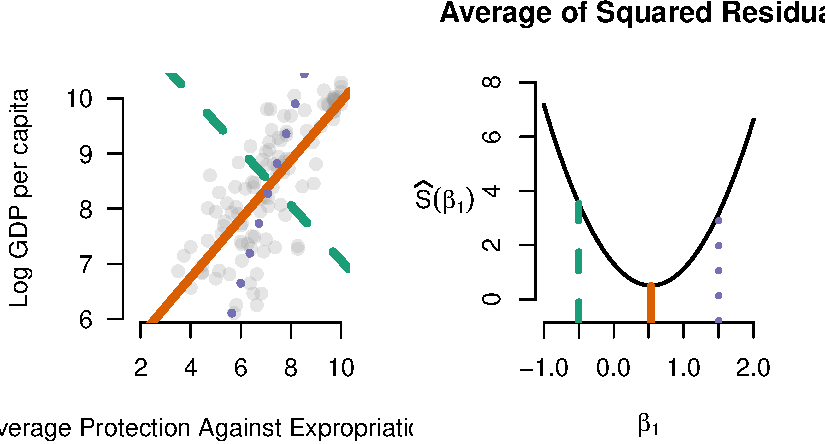
\includegraphics{07_least_squares_files/figure-pdf/fig-ssr-comp-1.pdf}

}

\caption{\label{fig-ssr-comp}Different possible lines and their
corresponding sum of squared residuals.}

\end{figure}

\hypertarget{model-fit}{%
\section{Model fit}\label{model-fit}}

We have learned how to use OLS to obtain an estimate of the best linear
predictor, but we may ask how good that prediction is. Does using
\(\X_i\) help us predict \(Y_i\)? To investigate this, we can consider
two different prediction errors: those using covariates and those that
do not.

We have already seen the prediction error when using the covariates; it
is just the \textbf{sum of the squared residuals}, \[ 
SSR = \sum_{i=1}^n (Y_i - \X_{i}'\bhat)^2.
\] Recall that the best predictor for \(Y_i\) without any covariates is
simply its sample mean \(\overline{Y}\), and so the prediction error
without covariates is what we call the \textbf{total sum of squares},
\[ 
TSS = \sum_{i=1}^n (Y_i - \overline{Y})^2.
\] Figure~\ref{fig-ssr-vs-tss} shows the difference between these two
types of prediction errors.

\begin{figure}

{\centering 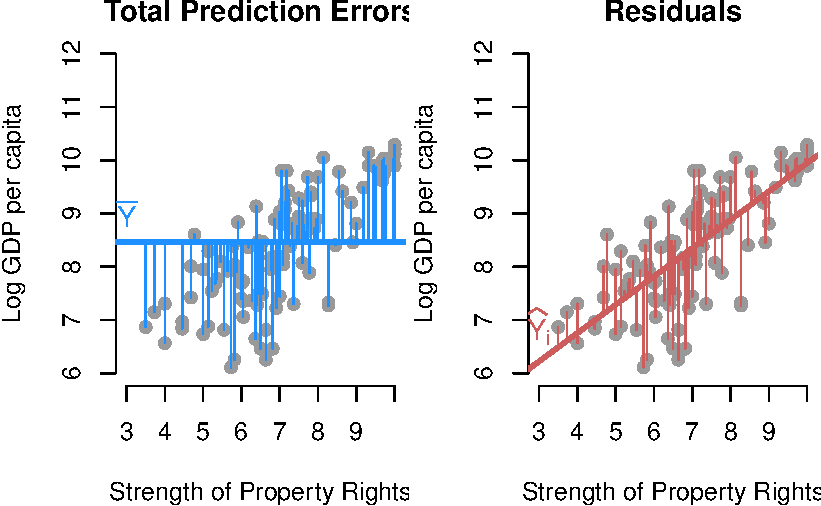
\includegraphics{07_least_squares_files/figure-pdf/fig-ssr-vs-tss-1.pdf}

}

\caption{\label{fig-ssr-vs-tss}Total sum of squares vs.~the sum of
squared residuals.}

\end{figure}

We can use the \textbf{proportion reduction in prediction error} from
adding those covariates to measure how much those covariates improve the
regression's predictive ability. This value, called the
\textbf{coefficient of determination} or \(R^2\), is simply \[
R^2 = \frac{TSS - SSR}{TSS} = 1-\frac{SSR}{TSS},
\] which is the reduction in error moving from \(\overline{Y}\) to
\(\X_i'\bhat\) as the predictor relative to the prediction error using
\(\overline{Y}\). We can think of this as the fraction of the total
prediction error eliminated by using \(\X_i\) to predict \(Y_i\). One
thing to note is that OLS will \emph{always} improve in-sample fit so
that \(TSS \geq SSR\) even if \(\X_i\) is unrelated to \(Y_i\). This
phantom improvement occurs because the whole point of OLS is to minimize
the SSR, and it will do that even if it is just chasing noise.

Since regression always improves in-sample fit, \(R^2\) will fall
between 0 and 1. A value 0 zero would indicate exactly 0 estimated
coefficients on all covariates (except the intercept) so that \(Y_i\)
and \(\X_i\) are perfectly orthogonal in the data (this is very unlikely
to occur because there will likely be some minimal but nonzero
relationship by random chance). A value of 1 indicates a perfect linear
fit.

\hypertarget{matrix-form-of-ols}{%
\section{Matrix form of OLS}\label{matrix-form-of-ols}}

While we derived the OLS estimator above, there is a much more common
representation of the estimator that relies on vectors and matrices. We
usually write the linear model for a generic unit,
\(Y_i = \X_i'\bfbeta + e_i\), but obviously, there are \(n\) of these
equations, \[ 
\begin{aligned}
  Y_1 &= \X_1'\bfbeta + e_1 \\
  Y_2 &= \X_2'\bfbeta + e_2 \\
  &\vdots \\
  Y_n &= \X_n'\bfbeta + e_n \\
\end{aligned}
\] We can write this system of equations in a more compact form using
matrix algebra. In particular, let's combine the variables here into
random vectors/matrices: \[
\mb{Y} = \begin{pmatrix}
Y_1 \\ Y_2 \\ \vdots \\ Y_n
  \end{pmatrix}, \quad
  \mathbb{X} = \begin{pmatrix}
\X'_1 \\
\X'_2 \\
\vdots \\
\X'_n
  \end{pmatrix} =
  \begin{pmatrix}
    1 & X_{11} & X_{12} & \cdots & X_{1k} \\
    1 & X_{21} & X_{22} & \cdots & X_{2k} \\
    \vdots & \vdots & \vdots & \vdots & \vdots \\
    1 & X_{n1} & X_{n2} & \cdots & X_{nk} \\
  \end{pmatrix},
  \quad
  \mb{e} = \begin{pmatrix}
e_1 \\ e_2 \\ \vdots \\ e_n
  \end{pmatrix}
\] Then we can write the above system of equations as \[
\mb{Y} = \mathbb{X}\bfbeta + \mb{e},
\] where notice now that \(\mathbb{X}\) is an \(n \times (k+1)\) matrix
and \(\bfbeta\) is a \(k+1\) length column vector.

A critical link between the definition of OLS above to the matrix
notation comes from representing sums in matrix form. In particular, we
have \[
\begin{aligned}
  \sum_{i=1}^n \X_i\X_i' &= \Xmat'\Xmat \\
  \sum_{i=1}^n \X_iY_i &= \Xmat'\mb{Y},
\end{aligned}
\] which means we can write the OLS estimator in the more recognizable
form as \[ 
\bhat = \left( \mathbb{X}'\mathbb{X} \right)^{-1} \mathbb{X}'\mb{Y}.
\]

Of course, we can also define the vector of residuals, \[ 
 \widehat{\mb{e}} = \mb{Y} - \mathbb{X}\bhat = \left[
\begin{array}{c}
    Y_1 \\
    Y_2 \\
    \vdots \\
    Y_n
    \end{array}
\right] - 
\left[
\begin{array}{c}
   1\widehat{\beta}_0 + X_{11}\widehat{\beta}_1 + X_{12}\widehat{\beta}_2 + \dots + X_{1k}\widehat{\beta}_k \\
   1\widehat{\beta}_0 + X_{21}\widehat{\beta}_1 + X_{22}\widehat{\beta}_2 + \dots + X_{2k}\widehat{\beta}_k \\
   \vdots \\
   1\widehat{\beta}_0 + X_{n1}\widehat{\beta}_1 + X_{n2}\widehat{\beta}_2 + \dots + X_{nk}\widehat{\beta}_k
\end{array}
\right],
\] and so the sum of the squared residuals, in this case, becomes \[ 
SSR(\bfbeta) = \Vert\mb{Y} - \mathbb{X}\bfbeta\Vert^{2} = (\mb{Y} - \mathbb{X}\bfbeta)'(\mb{Y} - \mathbb{X}\bfbeta),
\] where the double vertical lines mean the Euclidean norm of the
argument, \(\Vert \mb{z} \Vert = \sqrt{\sum_{i=1}^n z_i^{2}}\). The OLS
minimization problem, then, is \[ 
\bhat = \argmin_{\mb{b} \in \mathbb{R}^{(k+1)}}\; \Vert\mb{Y} - \mathbb{X}\mb{b}\Vert^{2}
\] Finally, we can write the orthogonality of the covariates and the
residuals as \[ 
\mathbb{X}'\widehat{\mb{e}} = \sum_{i=1}^{n} \X_{i}\widehat{e}_{i} = 0.
\]

\hypertarget{sec-rank}{%
\section{Rank, linear independence, and
multicollinearity}\label{sec-rank}}

When introducing the OLS estimator, we noted that it would exist when
\(\sum_{i=1}^n \X_i\X_i'\) is positive definite or that there is ``no
multicollinearity.'' This assumption is equivalent to saying that the
matrix \(\mathbb{X}\) is full column rank, meaning that
\(\text{rank}(\mathbb{X}) = (k+1)\), where \(k+1\) is the number of
columns of \(\mathbb{X}\). Recall from matrix algebra that the column
rank is the number of linearly independent columns in the matrix, and
\textbf{linear independence} means that \(\mathbb{X}\mb{b} = 0\) if and
only if \(\mb{b}\) is a column vector of 0s. In other words, we have \[ 
b_{1}\mathbb{X}_{1} + b_{2}\mathbb{X}_{2} + \cdots + b_{k+1}\mathbb{X}_{k+1} = 0 \quad\iff\quad b_{1} = b_{2} = \cdots = b_{k+1} = 0, 
\] where \(\mathbb{X}_j\) is the \(j\)th column of \(\mathbb{X}\). Thus,
full column rank says that all the columns are linearly independent or
that there is no ``multicollinearity.''

How could this be violated? Suppose we accidentally included a linear
function of one variable so that \(\mathbb{X}_2 = 2\mathbb{X}_1\). Then
we have, \[ 
\begin{aligned}
  \mathbb{X}\mb{b} &= b_{1}\mathbb{X}_{1} + b_{2}2\mathbb{X}_1+ b_{3}\mathbb{X}_{3}+ \cdots + b_{k+1}\mathbb{X}_{k+1} \\
  &= (b_{1} + 2b_{2})\mathbb{X}_{1} + b_{3}\mathbb{X}_{3} + \cdots + b_{k+1}\mathbb{X}_{k+1}
\end{aligned}
\] In this case, this expression equals 0 when
\(b_3 = b_4 = \cdots = b_{k+1} = 0\) and \(b_1 = -2b_2\). Thus, the
collection of columns is linearly dependent, so we know that the rank of
\(\mathbb{X}\) must be less than full column rank (that is, less than
\(k+1\)). Hopefully, it is also clear that if we removed the problematic
column \(\mathbb{X}_2\), the resulting matrix would have \(k\) linearly
independent columns, implying that \(\mathbb{X}\) is rank \(k\).

Why does this rank condition matter for the OLS estimator? A key
property of full column rank matrices is that \(\Xmat\) is of full
column rank if and only if \(\Xmat'\Xmat\) is non-singular and a matrix
is invertible if and only if it is non-singular. Thus, the columns of
\(\Xmat\) being linearly independent means that the inverse
\((\Xmat'\Xmat)^{-1}\) exists and so does \(\bhat\). Further, this full
rank condition also implies that
\(\Xmat'\Xmat = \sum_{i=1}^{n}\X_{i}\X_{i}'\) is positive definite,
implying that the estimator is truly finding the minimal sum of squared
residuals.

What are common situations that lead to violations of no
multicollinearity? We have seen one above, with one variable being a
linear function of another. But this problem can come out in more subtle
ways. Suppose that we have a set of dummy variables corresponding to a
single categorical variable, like the region of the country. In the US,
this might mean we have \(X_{i1} = 1\) for units in the West (0
otherwise), \(X_{i2} = 1\) for units in the Midwest (0 otherwise),
\(X_{i3} = 1\) for units in the South (0 otherwise), and \(X_{i4} = 1\)
for units in the Northeast (0 otherwise). Each unit has to be in one of
these four regions, so there is a linear dependence between these
variables, \[ 
X_{i4} = 1 - X_{i1} - X_{i2} - X_{i3}.
\] That is, if I know that you are not in the West, Midwest, or South
regions, I know that you are in the Northeast. We would get a linear
dependence if we tried to include all of these variables in our
regression with an intercept. (Note the 1 in the relationship between
\(X_{i4}\) and the other variables, that's why there will be linear
dependence when including a constant.) Thus, we usually omit one dummy
variable from each categorical variable. In that case, the coefficients
on the remaining dummies are differences in means between that category
and the omitted one (perhaps conditional on other variables included, if
included). So if we omitted \(X_{i4}\), then the coefficient on
\(X_{i1}\) would be the difference in mean outcomes between units in the
West and Northeast regions.

Another way collinearity can occur is if you include both an intercept
term and a variable that does not vary. This issue can often happen if
we mistakenly subset our data to, say, the West region but still include
the West dummy variable in the regression.

Finally, note that most statistical software packages will ``solve'' the
multicollinearity by arbitrarily removing as many linearly dependent
covariates as is necessary to achieve full rank. R will show the
estimated coefficients as \texttt{NA} in those cases.

\hypertarget{ols-coefficients-for-binary-and-categorical-regressors}{%
\section{OLS coefficients for binary and categorical
regressors}\label{ols-coefficients-for-binary-and-categorical-regressors}}

Suppose that the covariates include just the intercept and a single
binary variable, \(\X_i = (1\; X_{i})'\), where \(X_i \in \{0,1\}\). In
this case, the OLS coefficient on \(X_i\), \(\widehat{\beta_{1}}\), is
exactly equal to the difference in sample means of \(Y_i\) in the
\(X_i = 1\) group and the \(X_i = 0\) group: \[ 
\widehat{\beta}_{1} = \frac{\sum_{i=1}^{n} X_{i}Y_{i}}{\sum_{i=1}^{n} X_{i}} - \frac{\sum_{i=1}^{n} (1 - X_{i})Y_{i}}{\sum_{i=1}^{n} 1- X_{i}} = \overline{Y}_{X =1} - \overline{Y}_{X=0}
\] This result is not an approximation. It holds exactly for any sample
size.

We can generalize this idea to discrete variables more broadly. Suppose
we have our region variables from the last section and include in our
covariates a constant and the dummies for the West, Midwest, and South
regions. Then the coefficient on the West dummy will be \[ 
\widehat{\beta}_{\text{west}} = \overline{Y}_{\text{west}} - \overline{Y}_{\text{northeast}},
\] which is exactly the difference in sample means of \(Y_i\) between
the West region and units in the ``omitted region,'' the Northeast.

Note that these interpretations only hold when the regression consists
solely of the binary variable or the set of categorical dummy variables.
These exact relationships fail when other covariates are added to the
model.

\hypertarget{projection-and-geometry-of-least-squares}{%
\section{Projection and geometry of least
squares}\label{projection-and-geometry-of-least-squares}}

OLS has a very nice geometric interpretation that can add a lot of
intuition for various aspects of the method. In this geometric approach,
we view \(\mb{Y}\) as an \(n\)-dimensional vector in \(\mathbb{R}^n\).
As we saw above, OLS in matrix form is about finding a linear
combination of the covariate matrix \(\Xmat\) closest to this vector in
terms of the Euclidean distance (which is just the sum of squares).

Let
\(\mathcal{C}(\Xmat) = \{\Xmat\mb{b} : \mb{b} \in \mathbb{R}^(k+1)\}\)
be the \textbf{column space} of the matrix \(\Xmat\). This set is all
linear combinations of the columns of \(\Xmat\) or the set of all
possible linear predictions we could obtain from \(\Xmat\). Notice that
the OLS fitted values, \(\Xmat\bhat\), are in this column space. If, as
we assume, \(\Xmat\) has full column rank of \(k+1\), then the column
space \(\mathcal{C}(\Xmat)\) will be a \(k+1\)-dimensional surface
inside of the larger \(n\)-dimensional space. If \(\Xmat\) has two
columns, the column space will be a plane.

Another interpretation of the OLS estimator is that it finds the linear
predictor as the closest point in the column space of \(\Xmat\) to the
outcome vector \(\mb{Y}\). This is called the \textbf{projection} of
\(\mb{Y}\) onto \(\mathcal{C}(\Xmat)\). Figure~\ref{fig-projection}
shows this projection for a case with \(n=3\) and 2 columns in
\(\Xmat\). The shaded blue region represents the plane of the column
space of \(\Xmat\), and we can see that \(\Xmat\bhat\) is the closest
point to \(\mb{Y}\) in that space. That's the whole idea of the OLS
estimator: find the linear combination of the columns of \(\Xmat\) (a
point in the column space) that minimizes the Euclidean distance between
that point and the outcome vector (the sum of squared residuals).

\begin{figure}

{\centering 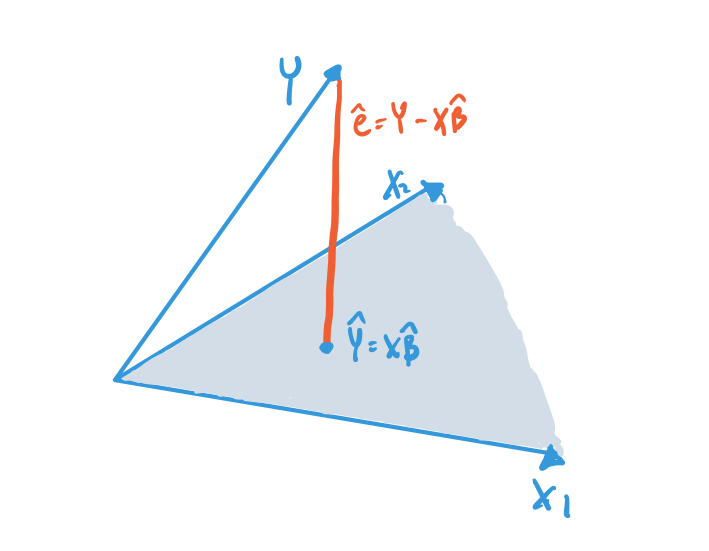
\includegraphics{assets/img/projection-drawing.png}

}

\caption{\label{fig-projection}Projection of Y on the column space of
the covariates.}

\end{figure}

This figure shows that the residual vector, which is the difference
between the \(\mb{Y}\) vector and the projection \(\Xmat\bhat\), is
perpendicular or orthogonal to the column space of \(\Xmat\). This
orthogonality is a consequence of the residuals being orthogonal to all
the columns of \(\Xmat\), \[ 
\Xmat'\mb{e} = 0,
\] as we established above. Being orthogonal to all the columns means it
will also be orthogonal to all linear combinations of the columns.

\hypertarget{projection-and-annihilator-matrices}{%
\section{Projection and annihilator
matrices}\label{projection-and-annihilator-matrices}}

Now that we have the idea of projection to the column space of
\(\Xmat\), we can define a way to project any vector into that space.
The \(n\times n\) \textbf{projection matrix,} \[
\mb{P}_{\Xmat} = \Xmat (\Xmat'\Xmat)^{-1} \Xmat',
\] projects a vector into \(\mathcal{C}(\Xmat)\). In particular, we can
see that this gives us the fitted values for \(\mb{Y}\): \[ 
\mb{P}_{\Xmat}\mb{Y} = \Xmat (\Xmat'\Xmat)^{-1} \Xmat'\mb{Y} = \Xmat\bhat.
\] Because we sometimes write the linear predictor as
\(\widehat{\mb{Y}} = \Xmat\bhat\), the projection matrix is also called
the \textbf{hat matrix}. With either name, multiplying a vector by
\(\mb{P}_{\Xmat}\) gives the best linear predictor of that vector as a
function of \(\Xmat\). Intuitively, any vector that is already a linear
combination of the columns of \(\Xmat\) (so is in
\(\mathcal{C}(\Xmat)\)) should be unaffected by this projection: the
closest point in \(\mathcal{C}(\Xmat)\) to a point already in
\(\mathcal{C}(\Xmat)\) is itself. We can also see this algebraically for
any linear combination \(\Xmat\mb{c}\), \[
\mb{P}_{\Xmat}\Xmat\mb{c} = \Xmat (\Xmat'\Xmat)^{-1} \Xmat'\Xmat\mb{c} = \Xmat\mb{c},
\] because \((\Xmat'\Xmat)^{-1} \Xmat'\Xmat\) simplifies to the identity
matrix. In particular, the projection of \(\Xmat\) onto itself is just
itself: \(\mb{P}_{\Xmat}\Xmat = \Xmat\).

The second matrix related to projection is the \textbf{annihilator
matrix}, \[ 
\mb{M}_{\Xmat} = \mb{I}_{n} - \mb{P}_{\Xmat},
\] which projects any vector into the orthogonal complement to the
column space of \(\Xmat\), \[
\mathcal{C}^{\perp}(\Xmat) = \{\mb{c} \in \mathbb{R}^n\;:\; \Xmat\mb{c} = 0 \}.
\] This matrix is called the annihilator matrix because if you apply it
to any linear combination of \(\Xmat\), you get 0: \[ 
\mb{M}_{\Xmat}\Xmat\mb{c} = \Xmat\mb{c} - \mb{P}_{\Xmat}\Xmat\mb{c} = \Xmat\mb{c} - \Xmat\mb{c} = 0,
\] and in particular, \(\mb{M}_{\Xmat}\Xmat = 0\). Why should we care
about this matrix? Perhaps a more evocative name might be the
\textbf{residual maker} since it makes residuals when applied to
\(\mb{Y}\), \[ 
\mb{M}_{\Xmat}\mb{Y} = (\mb{I}_{n} - \mb{P}_{\Xmat})\mb{Y} = \mb{Y} - \mb{P}_{\Xmat}\mb{Y} = \mb{Y} - \Xmat\bhat = \widehat{\mb{e}}.
\]

There are several fundamental properties of the projection matrix that
are useful:

\begin{itemize}
\item
  \(\mb{P}_{\Xmat}\) and \(\mb{M}_{\Xmat}\) are \textbf{idempotent},
  which means that when applied to itself, it simply returns itself:
  \(\mb{P}_{\Xmat}\mb{P}_{\Xmat} = \mb{P}_{\Xmat}\) and
  \(\mb{M}_{\Xmat}\mb{M}_{\Xmat} = \mb{M}_{\Xmat}\).
\item
  \(\mb{P}_{\Xmat}\) and \(\mb{M}_{\Xmat}\) are symmetric \(n \times n\)
  matrices so that \(\mb{P}_{\Xmat}' = \mb{P}_{\Xmat}\) and
  \(\mb{M}_{\Xmat}' = \mb{M}_{\Xmat}\).
\item
  The rank of \(\mb{P}_{\Xmat}\) is \(k+1\) (the number of columns of
  \(\Xmat\)) and the rank of \(\mb{M}_{\Xmat}\) is \(n - k - 1\).
\end{itemize}

We can use the projection and annihilator matrices to arrive at an
orthogonal decomposition of the outcome vector: \[ 
\mb{Y} = \Xmat\bhat + \widehat{\mb{e}} = \mb{P}_{\Xmat}\mb{Y} + \mb{M}_{\Xmat}\mb{Y}.
\]

\hypertarget{residual-regression}{%
\section{Residual regression}\label{residual-regression}}

There are many situations where we can partition the covariates into two
groups, and we might wonder if it is possible how to express or
calculate the OLS coefficients for just one set of covariates. In
particular, let the columns of \(\Xmat\) be partitioned into
\([\Xmat_{1} \Xmat_{2}]\), so that the linear prediction we are
estimating is \[ 
\mb{Y} = \Xmat_{1}\bfbeta_{1} + \Xmat_{2}\bfbeta_{2} + \mb{e}, 
\] with estimated coefficients and residuals \[ 
\mb{Y} = \Xmat_{1}\bhat_{1} + \Xmat_{2}\bhat_{2} + \widehat{\mb{e}}.
\]

We now document another way to obtain the estimator \(\bhat_1\) from
this regression using a technique called \textbf{residual regression},
\textbf{partitioned regression}, or the \textbf{Frisch-Waugh-Lovell
theorem}.

\begin{tcolorbox}[enhanced jigsaw, colbacktitle=quarto-callout-note-color!10!white, colframe=quarto-callout-note-color-frame, arc=.35mm, left=2mm, toptitle=1mm, rightrule=.15mm, title=\textcolor{quarto-callout-note-color}{\faInfo}\hspace{0.5em}{Residual regression approach}, colback=white, leftrule=.75mm, toprule=.15mm, coltitle=black, opacityback=0, breakable, bottomtitle=1mm, titlerule=0mm, bottomrule=.15mm, opacitybacktitle=0.6]

The residual regression approach is:

\begin{enumerate}
\def\labelenumi{\arabic{enumi}.}
\tightlist
\item
  Use OLS to regress \(\mb{Y}\) on \(\Xmat_2\) and obtain residuals
  \(\widetilde{\mb{e}}_2\).
\item
  Use OLS to regress each column of \(\Xmat_1\) on \(\Xmat_2\) and
  obtain residuals \(\widetilde{\Xmat}_1\).
\item
  Use OLS to regress \(\widetilde{\mb{e}}_{2}\) on
  \(\widetilde{\Xmat}_1\).
\end{enumerate}

\end{tcolorbox}

\begin{theorem}[Frisch-Waugh-Lovell]\protect\hypertarget{thm-fwl}{}\label{thm-fwl}

The OLS coefficients from a regression of \(\widetilde{\mb{e}}_{2}\) on
\(\widetilde{\Xmat}_1\) are equivalent to the coefficients on
\(\Xmat_{1}\) from the regression of \(\mb{Y}\) on both \(\Xmat_{1}\)
and \(\Xmat_2\).

\end{theorem}

One implication of this theorem is that the regression coefficient for a
given variable captures the relationship between the residual variation
in the outcome and that variable after accounting for the other
covariates. In particular, this coefficient focuses on the variation
orthogonal to those other covariates.

While perhaps unexpected, this result may not appear particularly
useful. We can just run the long regression, right? This trick can be
handy when \(\Xmat_2\) consists of dummy variables (or ``fixed
effects'') for a categorical variable with many categories. For example,
suppose \(\Xmat_2\) consists of indicators for the county of residence
for a respondent. In that case, that will have over 3,000 columns,
meaning that direct calculation of the
\(\bhat = (\bhat_{1}, \bhat_{2})\) will require inverting a matrix that
is bigger than \(3,000 \times 3,000\). Computationally, this process
will be very slow. But above, we saw that predictions of an outcome on a
categorical variable are just the sample mean within each level of the
variable. Thus, in this case, the residuals \(\widetilde{\mb{e}}_2\) and
\(\Xmat_1\) can be computed by demeaning the outcome and \(\Xmat_1\)
within levels of the dummies in \(\Xmat_2\), which can be considerably
faster computationally.

Finally, there are data visualization reasons to use residual
regression. It is often difficult to see if the linear functional form
for some covariate is appropriate once you begin to control for other
variables. One can check the relationship using this approach with a
scatterplot of \(\widetilde{\mb{e}}_2\) on \(\Xmat_1\) (when it is a
single column).

\hypertarget{outliers-leverage-points-and-influential-observations}{%
\section{Outliers, leverage points, and influential
observations}\label{outliers-leverage-points-and-influential-observations}}

Given that OLS finds the coefficients that minimize the sum of the
squared residuals, it is helpful to ask how much impact each residual
has on that solution. Let \(\bhat_{(-i)}\) be the OLS estimates if we
omit unit \(i\). Intuitively, \textbf{influential observations} should
significantly impact the estimated coefficients so that
\(\bhat_{(-i)} - \bhat\) is large in absolute value.

Under what conditions will we have influential observations? OLS tries
to minimize the sum of \textbf{squared} residuals, so it will move more
to shrink larger residuals than smaller ones. Where are large residuals
likely to occur? Well, notice that any OLS regression line with a
constant will go through the means of the outcome and the covariates:
\(\overline{Y} = \overline{\X}\bhat\). Thus, by definition, this means
that when an observation is close to the average of the covariates,
\(\overline{\X}\), it cannot have that much influence because OLS forces
the regression line to go through \(\overline{Y}\). Thus, we should look
for influential points that have two properties:

\begin{enumerate}
\def\labelenumi{\arabic{enumi}.}
\tightlist
\item
  Have high \textbf{leverage}, where leverage roughly measures how far
  \(\X_i\) is from \(\overline{\X}\), and
\item
  Be an \textbf{outlier} in the sense of having a large residual (if
  left out of the regression).
\end{enumerate}

We'll take each of these in turn.

\hypertarget{sec-leverage}{%
\subsection{Leverage points}\label{sec-leverage}}

We can define the \textbf{leverage} of an observation by \[ 
h_{ii} = \X_{i}'\left(\Xmat'\Xmat\right)^{-1}\X_{i},
\] which is the \(i\)th diagonal entry of the projection matrix,
\(\mb{P}_{\Xmat}\). Notice that \[ 
\widehat{\mb{Y}} = \mb{P}_{\Xmat}\mb{Y} \qquad \implies \qquad \widehat{Y}_i = \sum_{j=1}^n h_{ij}Y_j,
\] so that \(h_{ij}\) is the importance of observation \(j\) for the
fitted value for observation \(i\). The leverage, then, is the
importance of the observation for its own fitted value. We can also
interpret these values in terms of the distribution of \(\X_{i}\).
Roughly speaking, these values are the weighted distance \(\X_i\) is
from \(\overline{\X}\), where the weights normalize to the empirical
variance/covariance structure of the covariates (so that the scale of
each covariate is roughly the same). We can see this most clearly when
we fit a simple linear regression (with one covariate and an intercept)
with OLS when the leverage is \[ 
h_{ii} = \frac{1}{n} + \frac{(X_i - \overline{X})^2}{\sum_{j=1}^n (X_j - \overline{X})^2}
\]

Leverage values have three key properties:

\begin{enumerate}
\def\labelenumi{\arabic{enumi}.}
\tightlist
\item
  \(0 \leq h_{ii} \leq 1\)
\item
  \(h_{ii} \geq 1/n\) if the model contains an intercept
\item
  \(\sum_{i=1}^{n} h_{ii} = k + 1\)
\end{enumerate}

\hypertarget{outliers-and-leave-one-out-regression}{%
\subsection{Outliers and leave-one-out
regression}\label{outliers-and-leave-one-out-regression}}

In the context of OLS, an \textbf{outlier} is an observation with a
large prediction error for a particular OLS specification.
Figure~\ref{fig-outlier} shows an example of an outlier.

\begin{figure}

{\centering 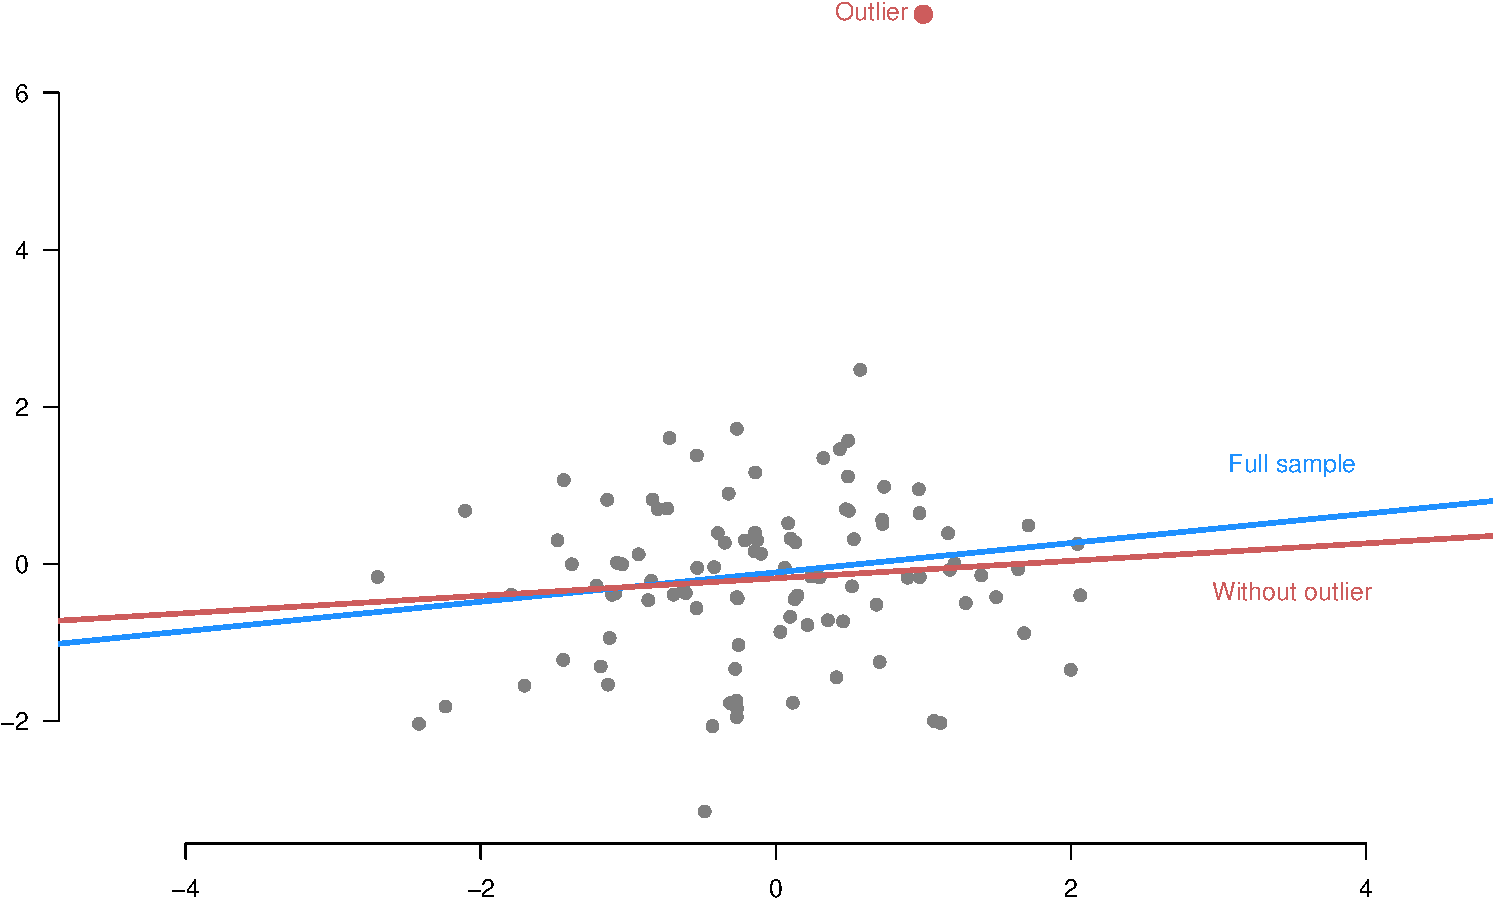
\includegraphics{07_least_squares_files/figure-pdf/fig-outlier-1.pdf}

}

\caption{\label{fig-outlier}An example of an outlier.}

\end{figure}

Intuitively, it seems as though we could use the residual
\(\widehat{e}_i\) to assess the prediction error for a given unit. But
the residuals are not valid predictions because the OLS estimator is
designed to make those as small as possible (in machine learning
parlance, these were in the training set). In particular, if an outlier
is influential, we already noted that it might ``pull'' the regression
line toward it, and the resulting residual might be pretty small.

To assess prediction errors more cleanly, we can use
\textbf{leave-one-out regression} (LOO), which regresses
\(\mb{Y}_{(-i)}\) on \(\Xmat_{(-i)}\), where these omit unit \(i\): \[ 
\bhat_{(-i)} = \left(\Xmat'_{(-i)}\Xmat_{(-i)}\right)^{-1}\Xmat_{(-i)}\mb{Y}_{(-i)}.
\] We can then calculate LOO prediction errors as \[ 
\widetilde{e}_{i} = Y_{i} - \X_{i}'\bhat_{(-i)}.
\] Calculating these LOO prediction errors for each unit appears to be
computationally costly because it seems as though we have to fit OLS
\(n\) times. Fortunately, there is a closed-form expression for the LOO
coefficients and prediction errors in terms of the original regression,
\begin{equation}\protect\hypertarget{eq-loo-coefs}{}{ 
\bhat_{(-i)} = \bhat - \left( \Xmat'\Xmat\right)^{-1}\X_i\widetilde{e}_i \qquad \widetilde{e}_i = \frac{\widehat{e}_i}{1 - h_{ii}}.
}\label{eq-loo-coefs}\end{equation} We can see from this that the LOO
prediction errors will differ from the residuals when the leverage of a
unit is high. This makes sense! We said earlier that observations with
low leverage would be close to \(\overline{\X}\), where the outcome
values have relatively little impact on the OLS fit (because the
regression line must go through \(\overline{Y}\)).

\hypertarget{influence-points}{%
\subsection{Influence points}\label{influence-points}}

An influence point is an observation that has the power to change the
coefficients and fitted values for a particular OLS specification.
Figure~\ref{fig-influence} shows an example of such an influence point.

\begin{figure}

{\centering 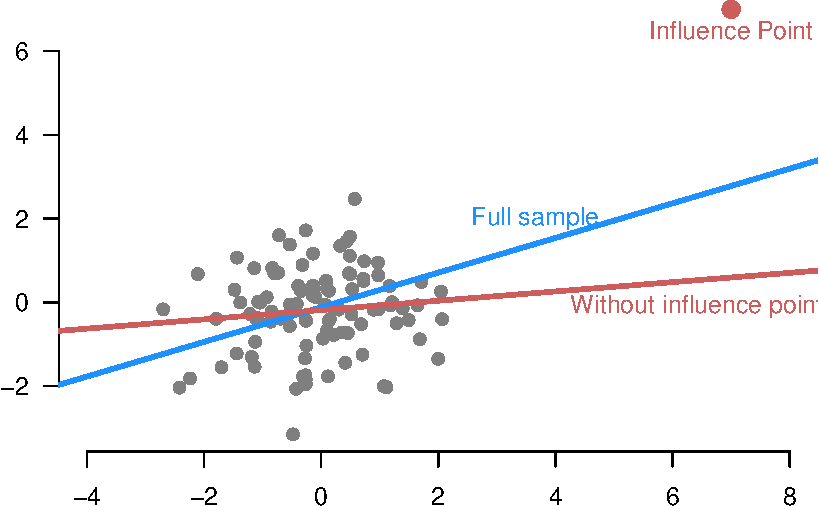
\includegraphics{07_least_squares_files/figure-pdf/fig-influence-1.pdf}

}

\caption{\label{fig-influence}An example of an influence point.}

\end{figure}

One measure of influence, called DFBETA\(_i\), measures how much \(i\)
changes the estimated coefficient vector \[ 
\bhat - \bhat_{(-i)} = \left( \Xmat'\Xmat\right)^{-1}\X_i\widetilde{e}_i,
\] so there is one value for each observation-covariate pair. When
divided by the standard error of the estimated coefficients, this is
called DFBETA\textbf{S} (where the ``S'' is for standardized). These are
helpful if we focus on a particular coefficient.

When we want to summarize how much an observation matters for the fit,
we can use a compact measure of the influence of an observation by
comparing the fitted value from the entire sample to the fitted value
from the leave-one-out regression. Using the DFBETA above, we have \[ 
\widehat{Y}_i - \X_{i}\bhat_{(-1)} = \X_{i}'(\bhat -\bhat_{(-1)}) = \X_{i}'\left( \Xmat'\Xmat\right)^{-1}\X_i\widetilde{e}_i = h_{ii}\widetilde{e}_i,
\] so the influence of an observation is its leverage times how much of
an outlier it is. This value is sometimes called DFFIT (difference in
fit). One transformation of this quantity, \textbf{Cook's distance},
standardizes this by the sum of the squared residuals: \[ 
D_i = \frac{n-k-1}{k+1}\frac{h_{ii}\widetilde{e}_{i}^{2}}{\widehat{\mb{e}}'\widehat{\mb{e}}}.
\] Various rules exist for establishing cutoffs for identifying an
observation as ``influential'' based on these metrics, but they tend to
be ad hoc. In any case, it's better to focus on the holistic question of
``how much does this observation matter for my substantive
interpretation'' rather than the narrow question of a particular
threshold.

It's all well and good to find influential points, but what should you
do about it? The first thing to check is that the data is not corrupted
somehow. Sometimes influence points occur because of a coding or data
entry error. If you have control over that coding, you should fix those
errors. You may consider removing the observation if the error appears
in the data acquired from another source. Still, when writing up your
analyses, you should be extremely transparent about this choice. Another
approach is to consider a transformation of the dependent or independent
variables, like the natural logarithm, that might dampen the effects of
outliers. Finally, consider using methods that are robust to outliers.

\hypertarget{the-statistics-of-least-squares}{%
\chapter{The statistics of least
squares}\label{the-statistics-of-least-squares}}

In the last chapter, we derived the least squares estimator and
investigated many of its mechanical properties. These properties are
essential for the practical application of OLS. Still, we should also
understand its statistical properties, such as the ones described in
Part I: unbiasedness, sampling variance, consistency, and asymptotic
normality. As we saw then, these properties fall into finite-sample
(unbiasedness, sampling variance) and asymptotic (consistency,
asymptotic normality).

In this chapter, we will focus first on the asymptotic properties of OLS
because those properties hold under the relatively mild conditions of
the linear projection model introduced in
Section~\ref{sec-linear-projection}. We will see that OLS consistently
estimates a coherent quantity of interest (the best linear predictor)
regardless of whether the conditional expectation is linear. That is,
for the asymptotic properties of the estimator, we will not need the
commonly invoked linearity assumption. Later, when we investigate the
finite-sample properties, we will show how linearity will help us
establish unbiasedness and how normality of the errors can allow us to
conduct exact, finite-sample inference. But these assumptions are very
strong, so it's vital to understand what we can say about OLS without
making them.

\hypertarget{large-sample-properties-of-ols}{%
\section{Large-sample properties of
OLS}\label{large-sample-properties-of-ols}}

As we saw in Chapter~\ref{sec-asymptotics}, we need two key ingredients
to conduct statistical inference with the OLS estimator: a consistent
estimate of the variance of \(\bhat\) and the approximate distribution
of \(\bhat\) in large samples. Remember that since \(\bhat\) is a
vector, the variance of that estimator will actually be a
variance-covariance matrix. To obtain these two ingredients, we will
first establish the consistency of OLS and then use the central limit
theorem to derive its asymptotic distribution, which will include its
variance.

We begin by setting out the assumptions we will need for establishing
the large-sample properties of OLS, which are the same as the
assumptions needed to ensure that the best linear predictor,
\(\bhat = \E[\X_{i}\X_{i}']^{-1}\E[\X_{i}Y_{i}]\), is well-defined and
unique.

\begin{tcolorbox}[enhanced jigsaw, colbacktitle=quarto-callout-note-color!10!white, colframe=quarto-callout-note-color-frame, arc=.35mm, left=2mm, toptitle=1mm, rightrule=.15mm, title=\textcolor{quarto-callout-note-color}{\faInfo}\hspace{0.5em}{Linear projection assumptions}, colback=white, leftrule=.75mm, toprule=.15mm, coltitle=black, opacityback=0, breakable, bottomtitle=1mm, titlerule=0mm, bottomrule=.15mm, opacitybacktitle=0.6]

The linear projection model makes the following assumptions:

\begin{enumerate}
\def\labelenumi{\arabic{enumi}.}
\item
  \(\{(Y_{i}, \X_{i})\}_{i=1}^n\) are iid random vectors
\item
  \(\E[Y^{2}_{i}] < \infty\) (finite outcome variance)
\item
  \(\E[\Vert \X_{i}\Vert^{2}] < \infty\) (finite variances and
  covariances of covariates)
\item
  \(\E[\X_{i}\X_{i}']\) is positive definite (no linear dependence in
  the covariates)
\end{enumerate}

\end{tcolorbox}

Recall that these are mild conditions on the joint distribution of
\((Y_{i}, \X_{i})\) and in particular, we are \textbf{not} assuming
linearity of the CEF, \(\E[Y_{i} \mid \X_{i}]\), nor are we assuming any
specific distribution for the data.

We can helpfully decompose the OLS estimator into the actual BLP
coefficient plus estimation error as \[ 
\bhat = \left( \frac{1}{n} \sum_{i=1}^n \X_i\X_i' \right)^{-1} \left( \frac{1}{n} \sum_{i=1}^n \X_iY_i \right) = \bfbeta + \underbrace{\left( \frac{1}{n} \sum_{i=1}^n \X_i\X_i' \right)^{-1} \left( \frac{1}{n} \sum_{i=1}^n \X_ie_i \right)}_{\text{estimation error}}.
\]

This decomposition will help us quickly establish the consistency of
\(\bhat\). By the law of large numbers, we know that sample means will
converge in probability to population expectations, so we have \[ 
\frac{1}{n} \sum_{i=1}^n \X_i\X_i' \inprob \E[\X_i\X_i'] \equiv \mb{Q}_{\X\X} \qquad \frac{1}{n} \sum_{i=1}^n \X_ie_i \inprob \E[\X_{i} e_{i}] = \mb{0},
\] which implies that \[
\bhat \inprob \bfbeta + \mb{Q}_{\X\X}^{-1}\E[\X_ie_i] = \bfbeta,
\] by the continuous mapping theorem (the inverse is a continuous
function). The linear projection assumptions ensure that LLN applies to
these sample means and that \(\E[\X_{i}\X_{i}']\) is invertible.

\begin{theorem}[]\protect\hypertarget{thm-ols-consistency}{}\label{thm-ols-consistency}

Under the above linear projection assumptions, the OLS estimator is
consistent for the best linear projection coefficients,
\(\bhat \inprob \bfbeta\).

\end{theorem}

Thus, OLS should be close to the population linear regression in large
samples under relatively mild conditions. Remember that this might not
equal the conditional expectation if the CEF is nonlinear. We can say
here that OLS converges to the best \emph{linear} approximation to the
CEF. Of course, this also means that if the CEF is linear, then OLS will
consistently estimate the coefficients of the CEF.

To emphasize here: the only assumption we made about the dependent
variable is that it has finite variance and is iid. Under this
assumption, the outcome could be continuous, categorical, binary, or
event count.

Next, we would like to establish an asymptotic normality result for the
OLS coefficients. We first review some key ideas about the central limit
theorem.

\begin{tcolorbox}[enhanced jigsaw, colbacktitle=quarto-callout-note-color!10!white, colframe=quarto-callout-note-color-frame, arc=.35mm, left=2mm, toptitle=1mm, rightrule=.15mm, title=\textcolor{quarto-callout-note-color}{\faInfo}\hspace{0.5em}{CLT reminder}, colback=white, leftrule=.75mm, toprule=.15mm, coltitle=black, opacityback=0, breakable, bottomtitle=1mm, titlerule=0mm, bottomrule=.15mm, opacitybacktitle=0.6]

Suppose that we have a function of the data iid random vectors
\(\X_1, \ldots, \X_n\), \(g(\X_{i})\) where \(\E[g(\X_{i})] = 0\) and so
\(\V[g(\X_{i})] = \E[g(\X_{i})g(\X_{i})']\). Then if
\(\E[\Vert g(\X_{i})\Vert^{2}] < \infty\), the CLT implies that
\begin{equation}\protect\hypertarget{eq-clt-mean-zero}{}{ 
\sqrt{n}\left(\frac{1}{n} \sum_{i=1}^{n} g(\X_{i}) - \E[g(\X_{i})]\right) = \frac{1}{\sqrt{n}} \sum_{i=1}^{n} g(\X_{i}) \indist \N(0, \E[g(\X_{i})g(\X_{i}')]) 
}\label{eq-clt-mean-zero}\end{equation}

\end{tcolorbox}

We now manipulate our decomposition to arrive at the \emph{stabilized}
version of the estimator, \[ 
\sqrt{n}\left( \bhat - \bfbeta\right) = \left( \frac{1}{n} \sum_{i=1}^n \X_i\X_i' \right)^{-1} \left( \frac{1}{\sqrt{n}} \sum_{i=1}^n \X_ie_i \right).
\] We have already established that the first term on the right-hand
side will converge in probability to \(\mb{Q}_{\X\X}^{-1}\). Notice that
\(\E[\X_{i}e_{i}] = 0\), so we can apply Equation~\ref{eq-clt-mean-zero}
to the second term. The covariance matrix of \(\X_ie_{i}\) is \[ 
\mb{\Omega} = \V[\X_{i}e_{i}] = \E[\X_{i}e_{i}(\X_{i}e_{i})'] = \E[e_{i}^{2}\X_{i}\X_{i}'].
\] The CLT will imply that \[ 
\frac{1}{\sqrt{n}} \sum_{i=1}^n \X_ie_i \indist \N(0, \mb{\Omega}).
\] Combining these facts with Slutsky's Theorem implies the following
theorem.

\begin{theorem}[]\protect\hypertarget{thm-ols-asymptotic-normality}{}\label{thm-ols-asymptotic-normality}

Suppose that the linear projection assumptions hold and, in addition, we
have \(\E[Y_{i}^{4}] < \infty\) and
\(\E[\lVert\X_{i}\rVert^{4}] < \infty\). Then the OLS estimator is
asymptotically normal with \[ 
\sqrt{n}\left( \bhat - \bfbeta\right) \indist \N(0, \mb{V}_{\bfbeta}),
\] where \[ 
\mb{V}_{\bfbeta} = \mb{Q}_{\X\X}^{-1}\mb{\Omega}\mb{Q}_{\X\X}^{-1} = \left( \E[\X_i\X_i'] \right)^{-1}\E[e_i^2\X_i\X_i']\left( \E[\X_i\X_i'] \right)^{-1}.
\]

\end{theorem}

Thus, if the sample size is large enough, we can approximate the
distribution of \(\bhat\) with a multivariate normal with mean
\(\bfbeta\) and covariance matrix \(\mb{V}_{\bfbeta}/n\). In particular,
the square root of the \(j\)th diagonals of this matrix will be standard
errors for \(\widehat{\beta}_j\). Knowing the shape of the OLS
estimator's multivariate distribution will allow us to conduct
hypothesis tests and generate confidence intervals for both individual
coefficients and groups of coefficients. But first, we need an estimate
of the covariance matrix!

\hypertarget{variance-estimation-for-ols}{%
\section{Variance estimation for
OLS}\label{variance-estimation-for-ols}}

The asymptotic normality of OLS from the last section is of limited
value without some way to estimate the covariance matrix, \[ 
\mb{V}_{\bfbeta} = \mb{Q}_{\X\X}^{-1}\mb{\Omega}\mb{Q}_{\X\X}^{-1}.
\] Since each term here is a population mean, this is an ideal place to
drop a plug-in estimator. In particular, let's use the following
estimators: \[ 
\begin{aligned}
  \mb{Q}_{\X\X} &= \E[\X_{i}\X_{i}'] & \widehat{\mb{Q}}_{\X\X} &= \frac{1}{n} \sum_{i=1}^{n} \X_{i}\X_{i}' = \frac{1}{n}\Xmat'\Xmat \\
  \mb{\Omega} &= \E[e_i^2\X_i\X_i'] & \widehat{\mb{\Omega}} & = \frac{1}{n}\sum_{i=1}^n\widehat{e}_i^2\X_i\X_i'.
\end{aligned}
\] Under the assumptions of Theorem~\ref{thm-ols-asymptotic-normality},
the LLN will imply that these are consistent for their targets,
\(\widehat{\mb{Q}}_{\X\X} \inprob \mb{Q}_{\X\X}\) and
\(\widehat{\mb{\Omega}} \inprob \mb{\Omega}\). We can plug these into
the variance formula to arrive at \[ 
\begin{aligned}
  \widehat{\mb{V}}_{\bfbeta} &= \widehat{\mb{Q}}_{\X\X}^{-1}\widehat{\mb{\Omega}}\widehat{\mb{Q}}_{\X\X}^{-1} \\
  &= \left( \frac{1}{n} \Xmat'\Xmat \right)^{-1} \left( \frac{1}{n} \sum_{i=1}^n\widehat{e}_i^2\X_i\X_i' \right) \left( \frac{1}{n} \Xmat'\Xmat \right)^{-1},
\end{aligned}
\] which by the continuous mapping theorem is consistent,
\(\widehat{\mb{V}}_{\bfbeta} \inprob \mb{V}_{\bfbeta}\).

This estimator is sometimes called the \textbf{robust variance
estimator} or, more accurately, the
\textbf{heteroskedasticity-consistent (HC) variance estimator}. How is
this robust? Consider the standard \textbf{homoskedasticity} assumption
that most statistical software packages make when estimating OLS
variances: the variance of the errors does not depend on the covariates:
\(\V[e_{i}^{2} \mid \X_{i}] = \V[e_{i}^{2}]\). This assumption is
stronger than we need, and we can rely on a weaker assumption that the
squared errors are uncorrelated with a specific function of the
covariates: \[ 
\E[e_{i}^{2}\X_{i}\X_{i}'] = \E[e_{i}^{2}]\E[\X_{i}\X_{i}'] = \sigma^{2}\mb{Q}_{\X\X}, 
\] where \(\sigma^2\) is the variance of the residuals (since
\(\E[e_{i}] = 0\)). Homoskedasticity simplifies the asymptotic variance
of the stabilized estimator, \(\sqrt{n}(\bhat - \bfbeta)\), to \[ 
\mb{V}^{\texttt{lm}}_{\bfbeta} = \mb{Q}_{\X\X}^{-1}\sigma^{2}\mb{Q}_{\X\X}\mb{Q}_{\X\X}^{-1} = \sigma^2\mb{Q}_{\X\X}^{-1}.
\] We already have an estimator for \(\mb{Q}_{\X\X}\), but we need one
for \(\sigma^2\). We can easily use the SSR, \[ 
\widehat{\sigma}^{2} = \frac{1}{n-k-1} \sum_{i=1}^{n} \widehat{e}_{i}^{2},
\] where we use \(n-k-1\) in the denominator instead of \(n\) to correct
for the residuals being slightly less variable than the actual errors
(because OLS mechanically attempts to make the residuals small). For
consistent variance estimation, \(n-k -1\) or \(n\) can be used, since
either way \(\widehat{\sigma}^2 \inprob \sigma^2\). Thus, under
homoskedasticity, we have \[ 
\widehat{\mb{V}}_{\bfbeta}^{\texttt{lm}} = \widehat{\sigma}^{2}\left(\Xmat'\Xmat\right)^{{-1}},
\] which is the standard variance estimator used by \texttt{lm()} in R
or \texttt{reg} in Stata.

Now that we have two estimators, \(\widehat{\mb{V}}_{\bfbeta}\) and
\(\widehat{\mb{V}}_{\bfbeta}^{\texttt{lm}}\), how do they compare?
Notice that the HC variance estimator and the homoskedasticity variance
estimator will both be consistent when homoskedasticity holds. But as
the ``heteroskedasticity-consistent'' label implies, only the HC
variance estimator will be consistent when homoskedasticity fails to
hold. So \(\widehat{\mb{V}}_{\bfbeta}\) has the advantage of being
consistent regardless of this assumption. This advantage comes at a
cost, however. When homoskedasticity is correct,
\(\widehat{\mb{V}}_{\bfbeta}^{\texttt{lm}}\) incorporates that
assumption into the estimator where the HC variance estimator has to
estimate it. The HC estimator will have higher variance (the variance
estimator will be more variable!) when homoskedasticity actually does
hold.

Now that we have established the asymptotic normality of the OLS
estimator and developed a consistent estimator of its variance, we can
proceed with all of the statistical inference tools we discussed in Part
I of this guide. Define the estimated
\textbf{heteroskedasticity-consistent standard errors} as \[ 
\widehat{\se}(\widehat{\beta}_{j}) = \sqrt{\frac{[\widehat{\mb{V}}_{\bfbeta}]_{jj}}{n}},
\] where \([\widehat{\mb{V}}_{\bfbeta}]_{jj}\) is the \(j\)th diagonal
entry of the HC variance estimator. Note that we divide by \(\sqrt{n}\)
here because \(\widehat{\mb{V}}_{\bfbeta}\) is a consistent estimator of
the stabilized estimator \(\sqrt{n}(\bhat - \bfbeta)\) not the estimator
itself.

Hypothesis tests and confidence intervals for individual coefficients
are almost precisely the same as with the general case presented in Part
I. For a two-sided test of \(H_0: \beta_j = b\) versus
\(H_1: \beta_j \neq b\), we can build the t-statistic and conclude that,
under the null, \[
\frac{\widehat{\beta}_j - b}{\widehat{\se}(\widehat{\beta}_{j})} \indist \N(0, 1).
\] Typically, statistical software will helpfully provide the
t-statistic for the null of no (partial) linear relationship between
\(X_{ij}\) and \(Y_i\), \[ 
t = \frac{\widehat{\beta}_{j}}{\widehat{\se}(\widehat{\beta}_{j})},
\] which measures how large the estimated coefficient is in standard
errors. With \(\alpha = 0.05\), asymptotic normality would imply that we
reject this null when \(t > 1.96\). We can form asymptotically-valid
confidence intervals with \[ 
\left[\widehat{\beta}_{j} - z_{\alpha/2}\;\widehat{\se}(\widehat{\beta}_{j}),\;\widehat{\beta}_{j} + z_{\alpha/2}\;\widehat{\se}(\widehat{\beta}_{j})\right]. 
\] For reasons we will discuss below, standard software typically relies
on the \(t\) distribution instead of the normal for hypothesis testing
and confidence intervals. Still, this difference is of little
consequence in large samples.

\hypertarget{inference-for-multiple-parameters}{%
\section{Inference for multiple
parameters}\label{inference-for-multiple-parameters}}

With multiple coefficients, we might have hypotheses that involve more
than one coefficient. As an example, let's focus on a regression with an
interaction between two covariates, \[
Y_i = \beta_0 + X_i\beta_1 + Z_i\beta_2 + X_iZ_i\beta_3 + e_i.
\] Suppose we wanted to test the hypothesis that \(X_i\) does not affect
the best linear predictor for \(Y_i\). That would be \[ 
H_{0}: \beta_{1} = 0 \text{ and } \beta_{3} = 0\quad\text{vs}\quad H_{1}: \beta_{1} \neq 0 \text{ or } \beta_{3} \neq 0,
\] where we usually write the null more compactly as
\(H_0: \beta_1 = \beta_3 = 0\).

To test this null hypothesis, we need a test statistic that
discriminates the two hypotheses: it should be large when the
alternative is true and small when the null is true. With a single
coefficient, we usually test the null hypothesis of
\(H_0: \beta_j = b_0\) with the \(t\)-statistic, \[ 
t = \frac{\widehat{\beta}_{j} - b_{0}}{\widehat{\se}(\widehat{\beta}_{j})},
\] and we usually take the absolute value, \(|t|\), as our measure of
how far our estimate is from the null. But notice that we could also use
the square of the \(t\) statistic, which is
\begin{equation}\protect\hypertarget{eq-squared-t}{}{ 
t^{2} = \frac{\left(\widehat{\beta}_{j} - b_{0}\right)^{2}}{\V[\widehat{\beta}_{j}]} = \frac{n\left(\widehat{\beta}_{j} - b_{0}\right)^{2}}{[\mb{V}_{\bfbeta}]_{[jj]}}. 
}\label{eq-squared-t}\end{equation}

So here's another way to differentiate the null from the alternative:
the squared distance between them divided by the variance of the
estimate.

Can we generalize this idea to hypotheses about multiple parameters?
Adding the sum of squared distances for each component of the null
hypothesis is straightforward. For our interaction example, that would
be \[ 
\widehat{\beta}_1^2 + \widehat{\beta}_3^2, 
\] but remember that some of the estimated coefficients are noisier than
others, so we should account for the uncertainty, just like we did for
the \(t\)-statistic.

With multiple parameters and multiple coefficients, the variances will
now require matrix algebra. We can write any hypothesis about linear
functions of the coefficients as \(H_{0}: \mb{L}\bfbeta = \mb{c}\). For
example, in the interaction case, we have \[ 
\mb{L} =
\begin{pmatrix}
  0 & 1 & 0 & 0 \\
  0 & 0 & 0 & 1 \\
\end{pmatrix}
\qquad
\mb{c} =
\begin{pmatrix}
  0 \\
  0
\end{pmatrix}
\] Thus, \(\mb{L}\bfbeta = \mb{0}\) is equivalent to \(\beta_1 = 0\) and
\(\beta_3 = 0\). Notice that with other \(\mb{L}\) matrices, we could
represent more complicated hypotheses like \(2\beta_1 - \beta_2 = 34\),
though we mostly stick to simpler functions. Let
\(\widehat{\bs{\theta}} = \mb{L}\bhat\) be the OLS estimate of the
function of the coefficients. By the delta method (discussed in
Section~\ref{sec-delta-method}), we have \[ 
\sqrt{n}\left(\mb{L}\bhat - \mb{L}\bfbeta\right) \indist \N(0, \mb{L}'\mb{V}_{\bfbeta}\mb{L}).
\] We can now generalize the squared \(t\) statistic in
Equation~\ref{eq-squared-t}. In particular, we will take the distances
\(\mb{L}\bhat - \mb{c}\) weighted by the variance-covariance matrix
\(\mb{L}'\mb{V}_{\bfbeta}\mb{L}\), \[ 
W = n(\mb{L}\bhat - \mb{c})'(\mb{L}'\mb{V}_{\bfbeta}\mb{L})^{-1}(\mb{L}\bhat - \mb{c}),
\] which is called the \textbf{Wald test statistic}. This statistic
generalizes the ideas of the t-statistic to multiple parameters. With
the t-statistic, we recenter to have mean 0 and divide by the standard
error to get a variance of 1. If we ignore the middle variance
weighting, we have \((\mb{L}\bhat - \mb{c})'(\mb{L}\bhat - \mb{c})\)
which is just the sum of the squared deviations of the estimates from
the null. Including the \((\mb{L}'\mb{V}_{\bfbeta}\mb{L})^{-1}\) weight
has the effect of rescaling the distribution of \(\mb{L}\bhat - \mb{c}\)
to make it rotationally symmetric around 0 (so the resulting dimensions
are uncorrelated) with each dimension having an equal variance of 1. In
this way, the Wald statistic transforms the random vectors to be
mean-centered and have variance 1 (just the t-statistic), but also to
have the resulting random variables in the vector be
uncorrelated.\footnote{The form of the Wald statistic is that of a
  weighted inner product, \(\mb{x}'\mb{Ay}\), where \(\mb{A}\) is a
  symmetric positive-definite weighting matrix.}

Why transform the data in this way? Figure~\ref{fig-wald} shows the
contour plot of a hypothetical joint distribution of two coefficients
from an OLS regression. We might want to know how far different points
in the distribution are from the mean, which in this case is \((1, 2)\).
Without considering the joint distribution, the circle is obviously
closer to the mean than the triangle. However, looking at where the two
points are on the distribution, the circle is at a lower contour than
the triangle, meaning it is more extreme than the triangle for this
particular distribution. The Wald statistic, then, takes into
consideration how much of a ``climb'' it is for \(\mb{L}\bhat\) to get
to \(\mb{c}\) given the distribution of \(\mb{L}\bhat\).

\begin{figure}

{\centering 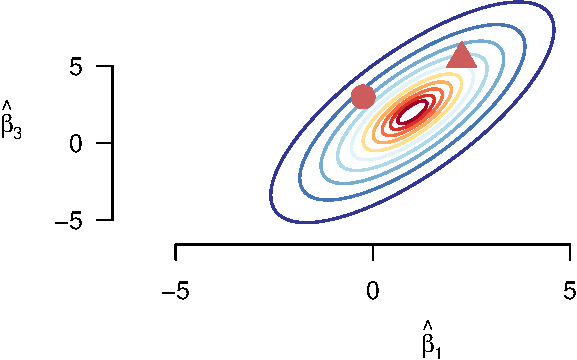
\includegraphics{08_ols_properties_files/figure-pdf/fig-wald-1.pdf}

}

\caption{\label{fig-wald}Hypothetical joint distribution of two slope
coefficients. The circle is closer to the center of the distribution by
the standard Euclidean distance, but the triangle is closer once you
consider the joint distribution.}

\end{figure}

If \(\mb{L}\) only has one row, our Wald statistic is the same as the
squared \(t\) statistic, \(W = t^2\). This fact will help us think about
the asymptotic distribution of \(W\). Notice that as \(n\to\infty\), we
know that by the asymptotic normality of \(\bhat\), \[ 
t = \frac{\widehat{\beta}_{j} - \beta_{j}}{\widehat{\se}[\widehat{\beta}_{j}]} \indist \N(0,1)
\] so \(t^2\) will converge in distribution to a \(\chi^2_1\) (since a
\(\chi^2_1\) is just one standard normal squared). After recentering and
rescaling by the covariance matrix, \(W\) converges to the sum of \(q\)
squared independent normals, where \(q\) is the number of rows of
\(\mb{L}\), or equivalently, the number of restrictions implied by the
null hypothesis. Thus, under the null hypothesis of
\(\mb{L}\bhat = \mb{c}\), we have \(W \indist \chi^2_{q}\).

\begin{tcolorbox}[enhanced jigsaw, colbacktitle=quarto-callout-note-color!10!white, colframe=quarto-callout-note-color-frame, arc=.35mm, left=2mm, toptitle=1mm, rightrule=.15mm, title=\textcolor{quarto-callout-note-color}{\faInfo}\hspace{0.5em}{Chi-squared critical values}, colback=white, leftrule=.75mm, toprule=.15mm, coltitle=black, opacityback=0, breakable, bottomtitle=1mm, titlerule=0mm, bottomrule=.15mm, opacitybacktitle=0.6]

We can obtain critical values for the \(\chi^2_q\) distribution using
the \texttt{qchisq()} function in R. For example, if we wanted to obtain
the critical value \(w\) that such that \(\P(W > w_{\alpha}) = \alpha\)
for our two-parameter interaction example, we could use:

\begin{Shaded}
\begin{Highlighting}[]
\FunctionTok{qchisq}\NormalTok{(}\AttributeTok{p =} \FloatTok{0.95}\NormalTok{, }\AttributeTok{df =} \DecValTok{2}\NormalTok{)}
\end{Highlighting}
\end{Shaded}

\begin{verbatim}
[1] 5.991465
\end{verbatim}

\end{tcolorbox}

We need to define the rejection region to use the Wald statistic in a
test. Because we are squaring each distance in \(W \geq 0\), larger
values of \(W\) indicate more disagreement with the null in either
direction. Thus, for an \(\alpha\)-level test of the joint null, we only
need a one-sided rejection region of the form
\(\P(W > w_{\alpha}) = \alpha\). Obtaining these values is
straightforward (see the above callout tip). For \(q = 2\) and a
\(\alpha = 0.05\), the critical value is roughly 6.

The Wald statistic is not a common test provided by standard statistical
software functions like \texttt{lm()} in R, though it is fairly
straightforward to implement ``by hand.'' Alternatively, packages like
\href{https://cran.r-project.org/web/packages/aod/index.html}{\texttt{\{aod\}}}
or
\href{http://jepusto.github.io/clubSandwich/}{\texttt{\{clubSandwich\}}}
have implementations of the test. What is reported by most software
implementations of OLS (like \texttt{lm()} in R) is the F-statistic,
which is \[ 
F = \frac{W}{q},
\] which also typically uses the homoskedastic variance estimator
\(\mb{V}^{\texttt{lm}}_{\bfbeta}\) in \(W\). The p-values reported for
such tests use the \(F_{q,n-k-1}\) distribution because this is the
exact distribution of the \(F\) statistic when the errors are (a)
homoskedastic and (b) normally distributed. When these assumptions do
not hold, the \(F\) distribution is not really statistically justified,
it is slightly more conservative than the \(\chi^2_q\) distribution, and
the inference will converge as \(n\to\infty\). So it might be justified
as an \emph{ad hoc} small sample adjustment to the Wald test. For
example, if we used the \(F_{q,n-k-1}\) with the interaction example
where \(q=2\) and say we have a sample size of \(n = 100\). In that
case, the critical value for the F test with \(\alpha = 0.05\) is

\begin{Shaded}
\begin{Highlighting}[]
\FunctionTok{qf}\NormalTok{(}\FloatTok{0.95}\NormalTok{, }\AttributeTok{df1 =} \DecValTok{2}\NormalTok{, }\AttributeTok{df2 =} \DecValTok{100} \SpecialCharTok{{-}} \DecValTok{4}\NormalTok{)}
\end{Highlighting}
\end{Shaded}

\begin{verbatim}
[1] 3.091191
\end{verbatim}

This result implies a critical value of 6.182 on the scale of the Wald
statistic (multiplying it by \(q = 2\)). Compared to the earlier
critical value of 5.991 based on the \(\chi^2_2\) distribution, we can
see that the inferences will be very similar even in moderately-sized
datasets.

Finally, note that the F-statistic reported by \texttt{lm()} in R is the
test of all the coefficients except the intercept being 0. In modern
quantitative social sciences, this test is seldom substantively
interesting.

\hypertarget{finite-sample-properties-with-a-linear-cef}{%
\section{Finite-sample properties with a linear
CEF}\label{finite-sample-properties-with-a-linear-cef}}

All the above results have been large-sample properties, and we have not
addressed finite-sample properties like the sampling variance or
unbiasedness. Under the linear projection assumption above, OLS is
generally biased without stronger assumptions. This section introduces
the stronger assumption that will allow us to establish stronger
properties for OLS. As usual, however, remember that these stronger
assumptions can be wrong.

\begin{tcolorbox}[enhanced jigsaw, colbacktitle=quarto-callout-note-color!10!white, colframe=quarto-callout-note-color-frame, arc=.35mm, left=2mm, toptitle=1mm, rightrule=.15mm, title=\textcolor{quarto-callout-note-color}{\faInfo}\hspace{0.5em}{Assumption: Linear Regression Model}, colback=white, leftrule=.75mm, toprule=.15mm, coltitle=black, opacityback=0, breakable, bottomtitle=1mm, titlerule=0mm, bottomrule=.15mm, opacitybacktitle=0.6]

\begin{enumerate}
\def\labelenumi{\arabic{enumi}.}
\item
  The variables \((Y_{i}, \X_{i})\) satisfy the linear CEF assumption.
  \[ 
  \begin{aligned}
    Y_{i} &= \X_{i}'\bfbeta + e_{i} \\
    \E[e_{i}\mid \X_{i}] & = 0.
  \end{aligned}
  \]
\item
  The design matrix is invertible \(\E[\X_{i}\X_{i}'] > 0\) (positive
  definite).
\end{enumerate}

\end{tcolorbox}

We discussed the concept of a linear CEF extensively in
Chapter~\ref{sec-regression}. However, recall that the CEF might be
linear mechanically if the model is \textbf{saturated} or when there are
as many coefficients in the model as there are unique values of
\(\X_i\). When a model is not saturated, the linear CEF assumption is
just that: an assumption. What can this assumption do? It can actually
establish quite a few nice statistical properties in finite samples.

One note before we proceed. When focusing on the finite sample inference
for OLS, it is customary to focus on its properties \textbf{conditional
on the observed covariates}, such as \(\E[\bhat \mid \Xmat]\) or
\(\V[\bhat \mid \Xmat]\). The historical reason for this was that the
researcher often chose these independent variables, so they were not
random. Thus, you'll sometimes see \(\Xmat\) treated as ``fixed'' in
some older texts, and they might even omit explicit conditioning
statements.

\begin{theorem}[]\protect\hypertarget{thm-ols-unbiased}{}\label{thm-ols-unbiased}

Under the linear regression model assumption, OLS is unbiased for the
population regression coefficients, \[
\E[\bhat \mid \Xmat] = \bfbeta,
\] and its conditional sampling variance is \[
\mb{\V}_{\bhat} = \V[\bhat \mid \Xmat] = \left( \Xmat'\Xmat \right)^{-1}\left( \sum_{i=1}^n \sigma^2_i \X_i\X_i' \right) \left( \Xmat'\Xmat \right)^{-1},
\] where \(\sigma^2_{i} = \E[e_{i}^{2} \mid \Xmat]\).

\end{theorem}

\begin{proof}

To prove the conditional unbiasedness, recall that we can write the OLS
estimator as \[
\bhat = \bfbeta + (\Xmat'\Xmat)^{-1}\Xmat'\mb{e},
\] and so taking (conditional) expectations, we have, \[
\E[\bhat \mid \Xmat] = \bfbeta + \E[(\Xmat'\Xmat)^{-1}\Xmat'\mb{e} \mid \Xmat] = \bfbeta + (\Xmat'\Xmat)^{-1}\Xmat'\E[\mb{e} \mid \Xmat] = \bfbeta,
\] because under the linear CEF assumption \(\E[\mb{e}\mid \Xmat] = 0\).

For the conditional sampling variance, we can use the same decomposition
we have, \[
\V[\bhat \mid \Xmat] = \V[\bfbeta + (\Xmat'\Xmat)^{-1}\Xmat'\mb{e} \mid \Xmat] = (\Xmat'\Xmat)^{-1}\Xmat'\V[\mb{e} \mid \Xmat]\Xmat(\Xmat'\Xmat)^{-1}. 
\] Since \(\E[\mb{e}\mid \Xmat] = 0\), we know that
\(\V[\mb{e}\mid \Xmat] = \E[\mb{ee}' \mid \Xmat]\), which is a matrix
with diagonal entries \(\E[e_{i}^{2} \mid \Xmat] = \sigma^2_i\) and
off-diagonal entries
\(\E[e_{i}e_{j} \Xmat] = \E[e_{i}\mid \Xmat]\E[e_{j}\mid\Xmat] = 0\),
where the first equality follows from the independence of the errors
across units. Thus, \(\V[\mb{e} \mid \Xmat]\) is a diagonal matrix with
\(\sigma^2_i\) along the diagonal, which means \[
\Xmat'\V[\mb{e} \mid \Xmat]\Xmat = \sum_{i=1}^n \sigma^2_i \X_i\X_i',
\] establishing the conditional sampling variance.

\end{proof}

Thus, for any realization of the covariates, \(\Xmat\), OLS is unbiased
for the true regression coefficients \(\bfbeta\). By the law of iterated
expectation, we also know that it is unconditionally unbiased\footnote{We
  are basically ignoring some edge cases when it comes to discrete
  covariates here. In particular, we assume that \(\Xmat'\Xmat\) is
  nonsingular with probability one. However, this can fail if we have a
  binary covariate since there is some chance (however slight) that the
  entire column will be all ones or all zeros, which would lead to a
  singular matrix \(\Xmat'\Xmat\). Practically this is not a big deal,
  but it does mean that we have to ignore this issue theoretically or
  focus on conditional unbiasedness.} as well since \[
\E[\bhat] = \E[\E[\bhat \mid \Xmat]] = \bfbeta. 
\] The difference between these two statements usually isn't incredibly
meaningful.

There are a lot of variances flying around, so it's helpful to review
them. Above, we derived the asymptotic variance of
\(\mb{Z}_{n} = \sqrt{n}(\bhat - \bfbeta)\), \[
\mb{V}_{\bfbeta} = \left( \E[\X_i\X_i'] \right)^{-1}\E[e_i^2\X_i\X_i']\left( \E[\X_i\X_i'] \right)^{-1},
\] which implies that the approximate variance of \(\bhat\) will be
\(\mb{V}_{\bfbeta} / n\) because \[
\bhat = \frac{Z_n}{\sqrt{n}} + \bfbeta \quad\implies\quad \bhat \overset{a}{\sim} \N(\bfbeta, n^{-1}\mb{V}_{\bfbeta}),
\] where \(\overset{a}{\sim}\) means approximately asymptotically
distributed as. Under the linear CEF, the conditional sampling variance
of \(\bhat\) has a similar form and will be similar to the\\
\[
\mb{V}_{\bhat} = \left( \Xmat'\Xmat \right)^{-1}\left( \sum_{i=1}^n \sigma^2_i \X_i\X_i' \right) \left( \Xmat'\Xmat \right)^{-1} \approx \mb{V}_{\bfbeta} / n.
\] In practice, these two derivations lead to basically the same
variance estimator. Recall the heteroskedastic-consistent variance
estimator \[
\widehat{\mb{V}}_{\bfbeta} = \left( \frac{1}{n} \Xmat'\Xmat \right)^{-1} \left( \frac{1}{n} \sum_{i=1}^n\widehat{e}_i^2\X_i\X_i' \right) \left( \frac{1}{n} \Xmat'\Xmat \right)^{-1},
\] is a valid plug-in estimator for the asymptotic variance and \[
\widehat{\mb{V}}_{\bhat} = n^{-1}\widehat{\mb{V}}_{\bfbeta}.
\] Thus, in practice, the asymptotic and finite-sample results under a
linear CEF justify the same variance estimator.

\hypertarget{linear-cef-model-under-homoskedasticity}{%
\subsection{Linear CEF model under
homoskedasticity}\label{linear-cef-model-under-homoskedasticity}}

If we are willing to make a homoskedasticity assumption on the errors,
we can derive even stronger results for OLS. Stronger assumptions
typically lead to stronger conclusions, but those conclusions may not be
robust to assumption violations. But homoskedasticity is such a
historically important assumption that statistical software
implementations of OLS like \texttt{lm()} in R assume it.

\begin{tcolorbox}[enhanced jigsaw, colbacktitle=quarto-callout-note-color!10!white, colframe=quarto-callout-note-color-frame, arc=.35mm, left=2mm, toptitle=1mm, rightrule=.15mm, title=\textcolor{quarto-callout-note-color}{\faInfo}\hspace{0.5em}{Assumption: Homoskedasticity with a linear CEF}, colback=white, leftrule=.75mm, toprule=.15mm, coltitle=black, opacityback=0, breakable, bottomtitle=1mm, titlerule=0mm, bottomrule=.15mm, opacitybacktitle=0.6]

In addition to the linear CEF assumption, we further assume that \[
\E[e_i^2 \mid \X_i] = \E[e_i^2] = \sigma^2,
\] or that variance of the errors does not depend on the covariates.

\end{tcolorbox}

\begin{theorem}[]\protect\hypertarget{thm-homoskedasticity}{}\label{thm-homoskedasticity}

Under a linear CEF model with homoskedastic errors, the conditional
sampling variance is \[
\mb{V}^{\texttt{lm}}_{\bhat} = \V[\bhat \mid \Xmat] = \sigma^2 \left( \Xmat'\Xmat \right)^{-1},
\] and the variance estimator \[
\widehat{\mb{V}}^{\texttt{lm}}_{\bhat} = \widehat{\sigma}^2 \left( \Xmat'\Xmat \right)^{-1} \quad\text{where,}\quad \widehat{\sigma}^2 = \frac{1}{n - k - 1} \sum_{i=1}^n \widehat{e}_i^2
\] is unbiased,
\(\E[\widehat{\mb{V}}^{\texttt{lm}}_{\bhat} \mid \Xmat] = \mb{V}^{\texttt{lm}}_{\bhat}\).

\end{theorem}

\begin{proof}

Under homoskedasticity \(\sigma^2_i = \sigma^2\) for all \(i\). Recall
that \(\sum_{i=1}^n \X_i\X_i' = \Xmat'\Xmat\). Thus, the conditional
sampling variance from Theorem~\ref{thm-ols-unbiased}, \[ 
\begin{aligned}
\V[\bhat \mid \Xmat] &= \left( \Xmat'\Xmat \right)^{-1}\left( \sum_{i=1}^n \sigma^2 \X_i\X_i' \right) \left( \Xmat'\Xmat \right)^{-1} \\ &= \sigma^2\left( \Xmat'\Xmat \right)^{-1}\left( \sum_{i=1}^n \X_i\X_i' \right) \left( \Xmat'\Xmat \right)^{-1} \\&= \sigma^2\left( \Xmat'\Xmat \right)^{-1}\left( \Xmat'\Xmat \right) \left( \Xmat'\Xmat \right)^{-1} \\&= \sigma^2\left( \Xmat'\Xmat \right)^{-1} = \mb{V}^{\texttt{lm}}_{\bhat}.
\end{aligned}
\]

For unbiasedness, we just need to show that
\(\E[\widehat{\sigma}^{2} \mid \Xmat] = \sigma^2\). Recall that we
defined \(\mb{M}_{\Xmat}\) as the residual-maker because
\(\mb{M}_{\Xmat}\mb{Y} = \widehat{\mb{e}}\). We can use this to connect
the residuals to the errors, \[ 
\mb{M}_{\Xmat}\mb{e} = \mb{M}_{\Xmat}\mb{Y} - \mb{M}_{\Xmat}\Xmat\bfbeta = \mb{M}_{\Xmat}\mb{Y} = \widehat{\mb{e}},
\] so \[
\V[\widehat{\mb{e}} \mid \Xmat] = \mb{M}_{\Xmat}\V[\mb{e} \mid \Xmat] = \mb{M}_{\Xmat}\sigma^2,
\] where the first equality is because
\(\mb{M}_{\Xmat} = \mb{I}_{n} - \Xmat (\Xmat'\Xmat)^{-1} \Xmat'\) is
constant conditional on \(\Xmat\). Notice that the diagonal entries of
this matrix are the variances of particular residuals \(\widehat{e}_i\)
and that the diagonal entries of the annihilator matrix are
\(1 - h_{ii}\) (since the \(h_{ii}\) are the diagonal entries of
\(\mb{P}_{\Xmat}\)). Thus, we have \[ 
\V[\widehat{e}_i \mid \Xmat] = \E[\widehat{e}_{i}^{2} \mid \Xmat] = (1 - h_{ii})\sigma^{2}.
\] In the last chapter, we established one property of these leverage
values in Section~\ref{sec-leverage}, namely
\(\sum_{i=1}^n h_{ii} = k+ 1\), so
\(\sum_{i=1}^n 1- h_{ii} = n - k - 1\) and we have \[ 
\begin{aligned}
  \E[\widehat{\sigma}^{2} \mid \Xmat] &= \frac{1}{n-k-1} \sum_{i=1}^{n} \E[\widehat{e}_{i}^{2} \mid \Xmat] \\
                                      &= \frac{\sigma^{2}}{n-k-1} \sum_{i=1}^{n} 1 - h_{ii} \\
                                      &= \sigma^{2}. 
\end{aligned}
\] This establishes
\(\E[\widehat{\mb{V}}^{\texttt{lm}}_{\bhat} \mid \Xmat] = \mb{V}^{\texttt{lm}}_{\bhat}\).

\end{proof}

Thus, under the linear CEF model and homoskedasticity of the errors, we
have an unbiased variance estimator that is a simple function of the sum
of squared residuals and the design matrix. Most statistical software
packages estimate standard errors using
\(\widehat{\mb{V}}^{\texttt{lm}}_{\bhat}\).

The final result we can derive for the linear CEF under homoskedasticity
is an optimality result. We might ask ourselves if there is another
estimator for \(\bfbeta\) that would outperform OLS in the sense of
having a lower sampling variance. Perhaps surprisingly, no linear
estimator for \(\bfbeta\) has a lower conditional variance, meaning that
OLS is the \textbf{best linear unbiased estimator}, often jovially
shortened to BLUE. This result is famously known as the Gauss-Markov
Theorem.

\begin{theorem}[]\protect\hypertarget{thm-gauss-markov}{}\label{thm-gauss-markov}

Let \(\widetilde{\bfbeta} = \mb{AY}\) be a linear and unbiased estimator
for \(\bfbeta\). Under the linear CEF model with homoskedastic errors,
\[
\V[\widetilde{\bfbeta}\mid \Xmat] \geq \V[\bhat \mid \Xmat]. 
\]

\end{theorem}

\begin{proof}

Note that if \(\widetilde{\bfbeta}\) is unbiased then
\(\E[\widetilde{\bfbeta} \mid \Xmat] = \bfbeta\) and so \[
\bfbeta = \E[\mb{AY} \mid \Xmat] = \mb{A}\E[\mb{Y} \mid \Xmat] = \mb{A}\Xmat\bfbeta,
\] which implies that \(\mb{A}\Xmat = \mb{I}_n\). Rewrite the competitor
as \(\widetilde{\bfbeta} = \bhat + \mb{BY}\) where, \[ 
\mb{B} = \mb{A} - \left(\Xmat'\Xmat\right)^{-1}\Xmat'.
\] and note that \(\mb{A}\Xmat = \mb{I}_n\) implies that
\(\mb{B}\Xmat = 0\). We now have \[ 
\begin{aligned}
  \widetilde{\bfbeta} &= \left( \left(\Xmat'\Xmat\right)^{-1}\Xmat' + \mb{B}\right)\mb{Y} \\
                      &= \left( \left(\Xmat'\Xmat\right)^{-1}\Xmat' + \mb{B}\right)\Xmat\bfbeta + \left( \left(\Xmat'\Xmat\right)^{-1}\Xmat' + \mb{B}\right)\mb{e} \\
                      &= \bfbeta + \mb{B}\Xmat\bfbeta + \left( \left(\Xmat'\Xmat\right)^{-1}\Xmat' + \mb{B}\right)\mb{e} \\
  &= \bfbeta + \left( \left(\Xmat'\Xmat\right)^{-1}\Xmat' + \mb{B}\right)\mb{e}
\end{aligned}
\] The variance of the competitor is, thus, \[ 
\begin{aligned}
  \V[\widetilde{\bfbeta} \mid \Xmat]
  &= \left( \left(\Xmat'\Xmat\right)^{-1}\Xmat' + \mb{B}\right)\V[\mb{e}\mid \Xmat]\left( \left(\Xmat'\Xmat\right)^{-1}\Xmat' + \mb{B}\right)' \\
  &= \sigma^{2}\left( \left(\Xmat'\Xmat\right)^{-1}\Xmat' + \mb{B}\right)\left( \Xmat\left(\Xmat'\Xmat\right)^{-1} + \mb{B}'\right) \\
  &= \sigma^{2}\left(\left(\Xmat'\Xmat\right)^{-1}\Xmat'\Xmat\left(\Xmat'\Xmat\right)^{-1} + \left(\Xmat'\Xmat\right)^{-1}\Xmat'\mb{B}' + \mb{B}\Xmat\left(\Xmat'\Xmat\right)^{-1} + \mb{BB}'\right)\\
  &= \sigma^{2}\left(\left(\Xmat'\Xmat\right)^{-1} + \mb{BB}'\right)\\
  &\geq \sigma^{2}\left(\Xmat'\Xmat\right)^{-1} \\
  &= \V[\bhat \mid \Xmat]
\end{aligned}
\] The first equality comes from the properties of covariance matrices;
the second is due to homoskedasticity; the fourth is due to
\(\mb{B}\Xmat = 0\), which implies that \(\Xmat'\mb{B}' = 0\) as well.
The fifth inequality holds because matrix products of the form
\(\mb{BB}'\) are positive definite if \(\mb{B}\) is of full rank (which
we have assumed it is).

\end{proof}

In this proof, we saw that the variance of the competing estimator had
variance
\(\sigma^2\left(\left(\Xmat'\Xmat\right)^{-1} + \mb{BB}'\right)\) which
we argued was ``greater than 0'' in the matrix sense, which is also
called positive definite. What does this mean practically? Remember that
any positive definite matrix must have strictly positive diagonal
entries and that the diagonal entries of \(\V[\bhat \mid \Xmat]\) and
\(V[\widetilde{\bfbeta}\mid \Xmat]\) are the variances of the individual
parameters, \(\V[\widehat{\beta}_{j} \mid \Xmat]\) and
\(\V[\widetilde{\beta}_{j} \mid \Xmat]\). Thus, the variances of the
individual parameters will be larger for \(\widetilde{\bfbeta}\) than
for \(\bhat\).

Many textbooks cite the Gauss-Markov theorem as a critical advantage of
OLS over other methods, but it's essential to recognize its limitations.
It requires linearity and homoskedastic error assumptions, which can be
false in many applications.

Finally, note that while we have shown this result for linear
estimators, Hansen (2022) proves a more general version of this result
that applies to any unbiased estimator.

\hypertarget{the-normal-linear-model}{%
\section{The normal linear model}\label{the-normal-linear-model}}

Finally, we add the strongest and thus least loved of the classical
linear regression assumption: (conditional) normality of the errors. The
historical reason to use this assumption was that finite-sample
inference hits a roadblock without some knowledge of the sampling
distribution of \(\bhat\). Under the linear CEF model, we saw that it
was unbiased, and under homoskedasticity, we could produce an unbiased
estimator of the conditional variance. But to do hypothesis testing or
generate confidence intervals, we need to be able to make probability
statements about the estimator, and for that, we need to know its exact
distribution. When the sample size is large, we can rely on the CLT and
know it is approximately normal. But in small samples, what do we do?
Historically, we decided to assume (conditional) normality of the errors
to proceed with some knowledge that we were wrong but hopefully not too
wrong.

\begin{tcolorbox}[enhanced jigsaw, colbacktitle=quarto-callout-note-color!10!white, colframe=quarto-callout-note-color-frame, arc=.35mm, left=2mm, toptitle=1mm, rightrule=.15mm, title=\textcolor{quarto-callout-note-color}{\faInfo}\hspace{0.5em}{The normal linear regression model}, colback=white, leftrule=.75mm, toprule=.15mm, coltitle=black, opacityback=0, breakable, bottomtitle=1mm, titlerule=0mm, bottomrule=.15mm, opacitybacktitle=0.6]

In addition to the linear CEF assumption, we assume that \[
e_i \mid \Xmat \sim \N(0, \sigma^2).
\]

\end{tcolorbox}

A couple of things to point out:

\begin{itemize}
\tightlist
\item
  The assumption here is not that \((Y_{i}, \X_{i})\) are jointly normal
  (though this would be sufficient for the assumption to hold), but
  rather that \(Y_i\) is normally distributed conditional on \(\X_i\).
\item
  Notice that the normal regression model has the homoskedasticity
  assumption baked in.
\end{itemize}

\begin{theorem}[]\protect\hypertarget{thm-normal-ols}{}\label{thm-normal-ols}

Under the normal linear regression model, we have \[ 
\begin{aligned}
  \bhat \mid \Xmat &\sim \N\left(\bfbeta, \sigma^{2}\left(\Xmat'\Xmat\right)^{-1}\right) \\
  \frac{\widehat{\beta}_{j} - \beta_{j}}{[\widehat{\mb{V}}^{\texttt{lm}}_{\bhat}]_{jj}/\sqrt{n}} &\sim t_{n-k-1} \\
  W/q &\sim F_{q, n-k-1}. 
\end{aligned}
\]

\end{theorem}

This theorem says that in the normal linear regression model, the
coefficients follow a normal distribution, the t-statistics follow a
\(t\)-distribution, and a transformation of the Wald statistic follows
an \(F\) distribution. These are \textbf{exact} results and do not rely
on large-sample approximations. Under the assumption of conditional
normality of the errors, they are as valid for \(n = 5\) as for
\(n = 500,000\).

Few people believe errors follow a normal distribution, so why even
present these results? Unfortunately, most statistical software
implementations of OLS implicitly assume this when calculating p-values
for tests or constructing confidence intervals. That is, the p-value
associated with the \(t\)-statistic that \texttt{lm()} outputs in R
relies on the \(t_{n-k-1}\) distribution, and the critical values used
to construct confidence intervals with \texttt{confint()} use that
distribution as well. When normality does not hold, there is no
principled reason to use the \(t\) or the \(F\) distributions in this
way. But we might hold our nose and use this \emph{ad hoc} procedure
under two rationalizations:

\begin{itemize}
\tightlist
\item
  \(\bhat\) is asymptotically normal, but this approximation might be
  poor in smaller finite samples. The \(t\) distribution will make
  inference more conservative in these cases (wider confidence
  intervals, smaller test rejection regions), which might help offset
  the poor approximation of the normal in small samples.
\item
  As \(n\to\infty\), the \(t_{n-k-1}\) will converge to a standard
  normal distribution, so the \emph{ad hoc} adjustment will not matter
  much for medium to large samples.
\end{itemize}

These arguments are not very convincing since it's unclear whether the
\(t\) approximation will be any better than the normal in finite
samples. But it's the best we can do to console ourselves as we find
more data.

\bookmarksetup{startatroot}

\hypertarget{references}{%
\chapter*{References}\label{references}}
\addcontentsline{toc}{chapter}{References}

\markboth{References}{References}

\hypertarget{refs}{}
\begin{CSLReferences}{1}{0}
\leavevmode\vadjust pre{\hypertarget{ref-Hansen22}{}}%
Hansen, Bruce E. 2022. {``A {Modern Gauss}--{Markov Theorem}.''}
\emph{Econometrica} 90 (3): 1283--94.
\url{https://doi.org/10.3982/ECTA19255}.

\leavevmode\vadjust pre{\hypertarget{ref-Senn12}{}}%
Senn, Stephen. 2012. {``Tea for Three: Of Infusions and Inferences and
Milk in First.''} \emph{Significance} 9 (6): 30--33.
https://doi.org/\url{https://doi.org/10.1111/j.1740-9713.2012.00620.x}.

\end{CSLReferences}



\end{document}
